\documentclass[12pt]{ociamthesis}  % default square logo 
%\documentclass[12pt,beltcrest]{ociamthesis} % use old belt crest logo
%\documentclass[12pt,shieldcrest]{ociamthesis} % use older shield crest logo

%load any additional packages
\usepackage{amssymb}
\usepackage{indentfirst}
\usepackage{bm}
\usepackage{hyperref}
\hypersetup{
    colorlinks,
    citecolor=black,
    filecolor=black,
    linkcolor=black,
    urlcolor=black
}

%% QUOTATIONS MARKS
\usepackage{dirtytalk}

%% ULE COVER
\usepackage{pdfpages}

%% ITEMIZE
\usepackage{enumitem}

%% TABULAR
\usepackage{tabularx,booktabs}
\newcolumntype{C}[1]{>{\centering\let\newline\\\arraybackslash\hspace{0pt}}m{#1}}
\usepackage{multirow}

%% PSEUDO CODE
\usepackage{algorithm}
\usepackage[noend]{algpseudocode}

% TABLE
\usepackage{color}
\usepackage{adjustbox}

%% FANCY MATH
\usepackage{amsmath}
\usepackage{booktabs,array}
\usepackage{caption}
\usepackage{textcomp}

%URL
\usepackage{hyperref}

%WIDE FIGURES
\usepackage{graphicx}
\usepackage{caption}
\usepackage{subcaption}

%REFERENCES
\usepackage[backend=bibtex, style = ieee, urldate = comp]{biblatex}
\usepackage{xpatch}
\usepackage{url}
\usepackage{filecontents}

\bibliography{refs.bib}        %use a bibtex bibliography file refs.bib

\newcommand{\tableequation}[1]{%
  \vspace*{-\baselineskip}
  {\begin{flalign}#1&&&\end{flalign}}%
  \vspace*{-\baselineskip}
}


%input macros (i.e. write your own macros file called mymacros.tex 
%and uncomment the next line)
%\include{mymacros}

\title{Genetic algorithms applied\\[0.8ex] 
in Computer Fluid Dynamics for\\[0.8ex] 
multiobjective optimizationn}   %note \\[1ex] is a line break in the title

\author{Javier Lobato Perez}             %your name
\college{University of Vermont}  %your college

%\renewcommand{\submittedtext}{change the default text here if needed}
\degree{Bachelor of Science in Aerospace Engineering}     %the degree
\degreedate{May 2018}             %the degree date

%end the preamble and start the document
\begin{document}

%this baselineskip gives sufficient line spacing for an examiner to easily
%markup the thesis with comments
\baselineskip=18pt plus1pt

%set the number of sectioning levels that get number and appear in the contents
\setcounter{secnumdepth}{3}
\setcounter{tocdepth}{2}

% change from UVM cover to ULE cover
%\maketitle                  % create a title page from the preamble info
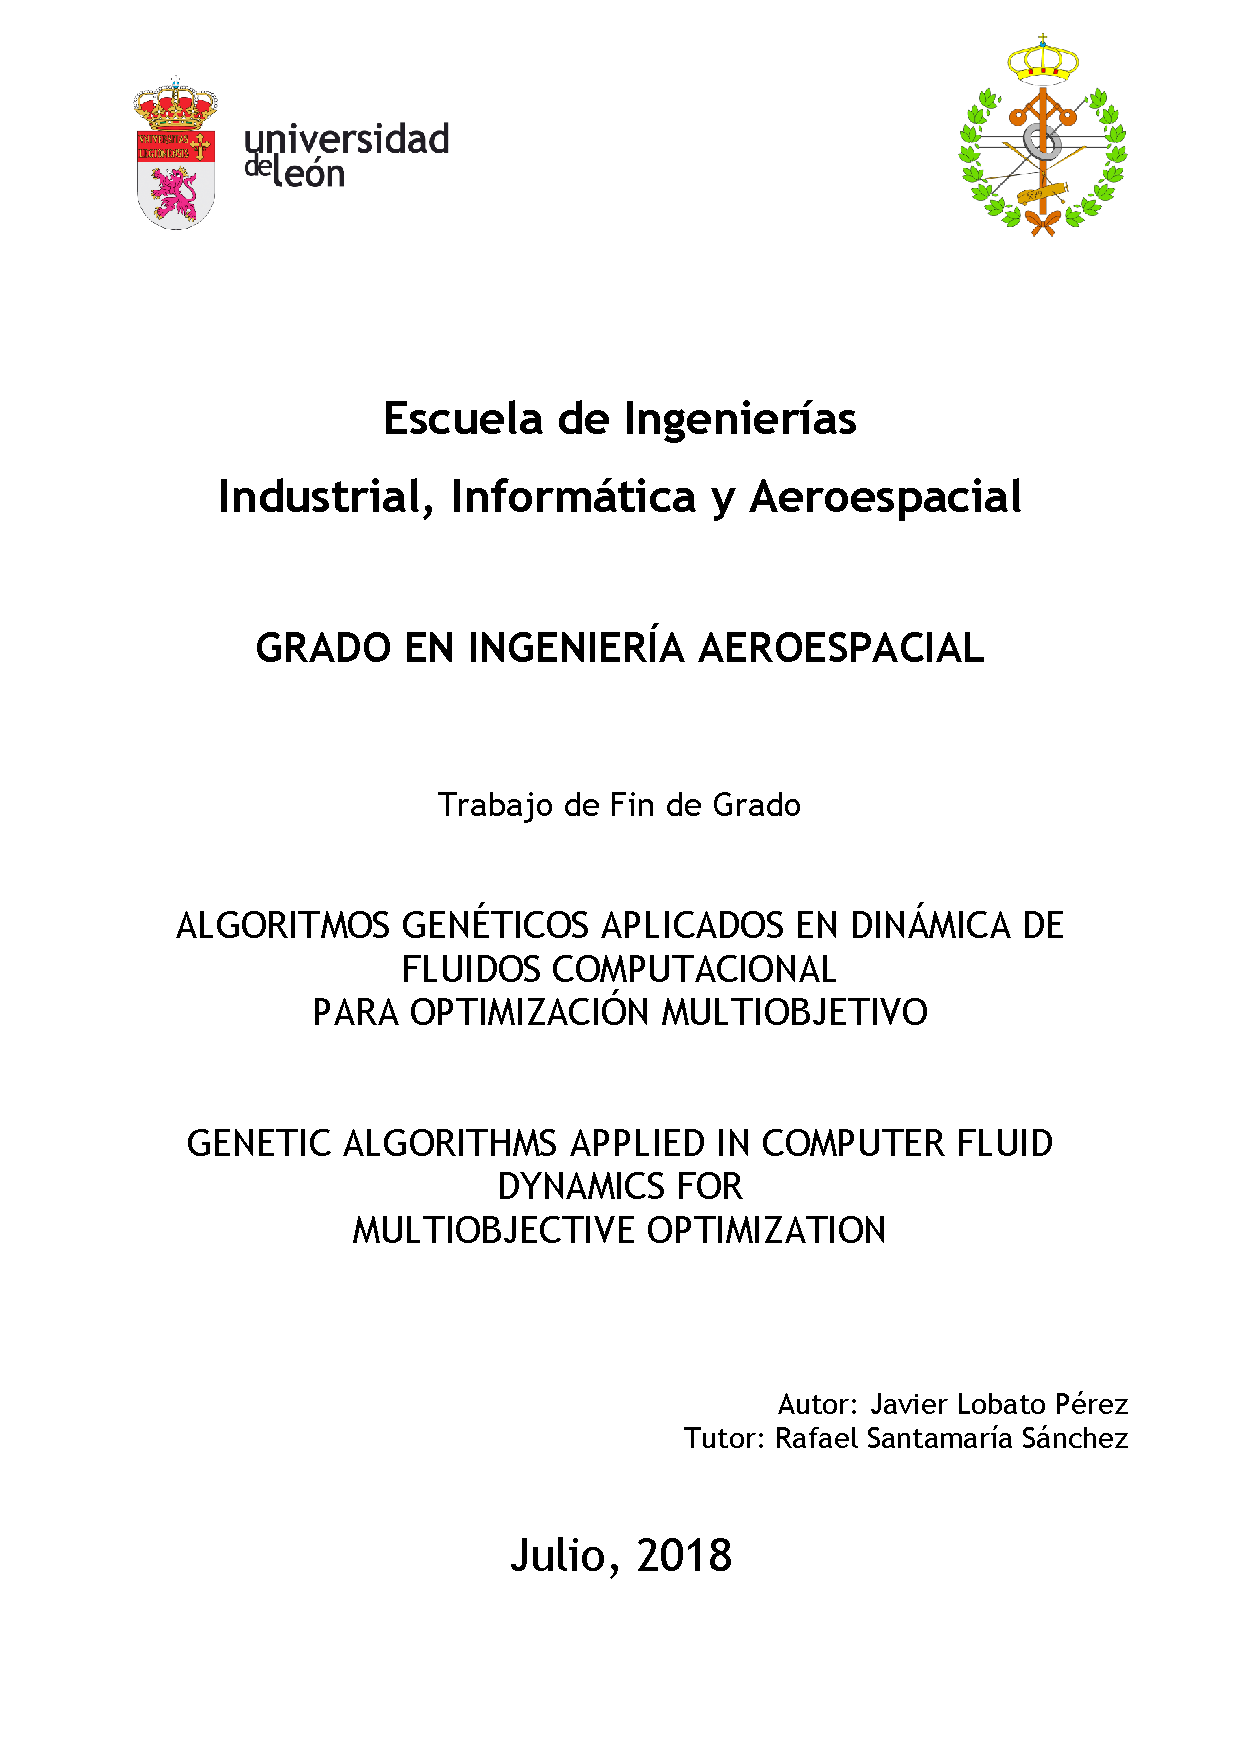
\includepdf[pages={1}]{files/ULEcover.pdf}


\begin{dedication}
This thesis is dedicated to\\
 my family\\
for being the greatest source of support\\
\end{dedication}        % include a dedication.tex file
\begin{acknowledgements}

I am grateful to my Thesis Advisor, Professor Yves Dubief, for all the support given throughout the whole process of developing this project. The computational resources provided let me perform the required simulations for drawing conclusions and getting results. I would also like to thank Professor Maggie Eppstein for the help with the genetic algorithm topics and also other professors whose support has also been helpful for this Senior Thesis.

I will also like to thank the whole community for the indirect help: Python as the programming language used and OpenFOAM for being the whole complete simulation suite with powerful characteristics. Also, the webpage \texttt{stack-overflow} for being the reference website for solving most of the programming questions that I have while developing the code. 

And finally, last but by no means least, to my parents, whose support and encouragement have helped me in the way, to my sister, for the positive feedback provided, to Ines, for being a major pillar every day, to Alberto and Veronica, for the hard-work nights in Votey, to Pablo, for some useful Python commands, and to everyone else that surely has had impact in this Senior Thesis.

\end{acknowledgements}   % include an acknowledgements.tex file
\begin{abstract}


The use of optimization in computational fluid dynamics for  engineering situations is a trending topic that is gaining a lot of attention. This study was focused on applying an optimization method to different computer fluid dynamics cases. Instead of using adjoint methods, genetic algorithms were used for the optimization process. The research was conducted with three different cases: vortex shedding in a cylinder wake (for minimizing the oscillations), diffuser inlet design (for maximizing the pressure ratio and Mach number) and airfoil shape optimization (different optimization configurations were tested). For these three cases, multiobjective optimization was imposed, having Pareto fronts with solutions that coexist in a trade-off situation rather than a single optimum point. The simulations produced promising results, showing that the approach is more than viable: it is a robust, adaptable and versatile way of optimizing engineering systems. Apart from the high level of parallelization and the automation of the procedure, the straightforward implementation allows that subtle changes in the code will optimize very different cases. Although the Pareto front was determined for the different cases, future work should be performed to increase the convergence of the method while reducing the number of simulations, given that they are a very time-consuming operation. 


\end{abstract}          % include the abstract

\begin{romanpages}          % start roman page numbering
\tableofcontents            % generate and include a table of contents
\listoffigures              % generate and include a list of figures
\listoftables              % generate and include a list of tables
\end{romanpages}            % end roman page numbering

%now include the files of latex for each of the chapters etc
\chapter{Introduction}

Optimization problems are everywhere, especially in engineering. Achieving the highest performance and increasing as much as possible the efficiency while reducing the costs are some of the objectives that every design tries to achieve. Finding the optimum is not always easy. In complex cases, the physics and the models used cannot be analyzed as a plain mathematical function from which extra information may be extracted to get the optimum solution. 

In those cases, machine learning is one of the tools that are in constant rise for problems from all disciplines. One of any of its different subdisciplines is almost always suitable to achieve a particular solution for one specific problem. 

As an aerospace engineering, the use of Computer Fluid Dynamics is essential for the analysis of aerodynamics and heat transfer problems. In order to optimize different engineering systems, the use of computer fluid dynamics to obtain accurate solutions appears to be one of the best tools. Combining this with some optimization techniques taken from machine learning will create a robust toolbox to perform optimization problems and apply them to engineering. 
\chapter{Literature review}
    
    Before moving into the different cases and simulations carried out, an extensive analysis of the current state-of-art must be done: beginning from the basics and going through the latest papers. The study will be structured in the three main parts of the thesis: optimization of multi-objective problems, genetic algorithms and computer fluid dynamics.

\section{Optimization}

    Most parts of the real-life engineering problems face not one but more variables to be optimized. The value of those variables is tried to be minimized or maximized depending on the case. However, in both cases, the idea is to get the optimum value. Those kinds of problems are called \textit{multi-objective optimization} (usually shortened as MO) given that there is more than one objective that is wanted to be optimized. The main difficulty is that those objectives are usually in conflict with each other, i.e. there is not a point where the solution is optimal (in the sense that it minimizes/maximizes all the objectives).
    
    The formal definition of multi-objective optimization is \cite{nonlinear}:
    \begin{equation}
        \begin{array}{cl}
            \textrm{minimize} & \{f_1(\bm{x}),f_2(\bm{x}),...,f_k(\bm{x})\} \\
            \textrm{subject to} & \bm{x} \in S
        \end{array}
        \label{eq:multiobjectiveDefnition}
    \end{equation}
    where there are $k$ objective functions that should be minimized ($k > 2$). The decision vector $\bm{x}$ contains the $n$ variables $\bm{x}=(x_1,x_2,...,x_n)$ of the $k$ functions and it must belong to a nonempty set $S$ of the search space. $S$ is also called the feasible set of the search space and it is usually described by constraint functions (in addition to some upper and lower bounds for each variable). Optimization problems are usually described to minimize a function, but maximize the function $f_i(\bm{x})$ is equivalent to minimize the function $-f_i(\bm{x})$.
    
    \newpage
    
    It must be noted that there are two spaces in which the optimization works: parameter or search space (denoted with $S$ in the literature) and optimization, objective or function space (denoted with $Z$). The number of search space variables may be different from the number of variables in the function space. These different designations will be interchangeable during the oncoming discussion. 
    
    \begin{figure}[h!]
        \centering
        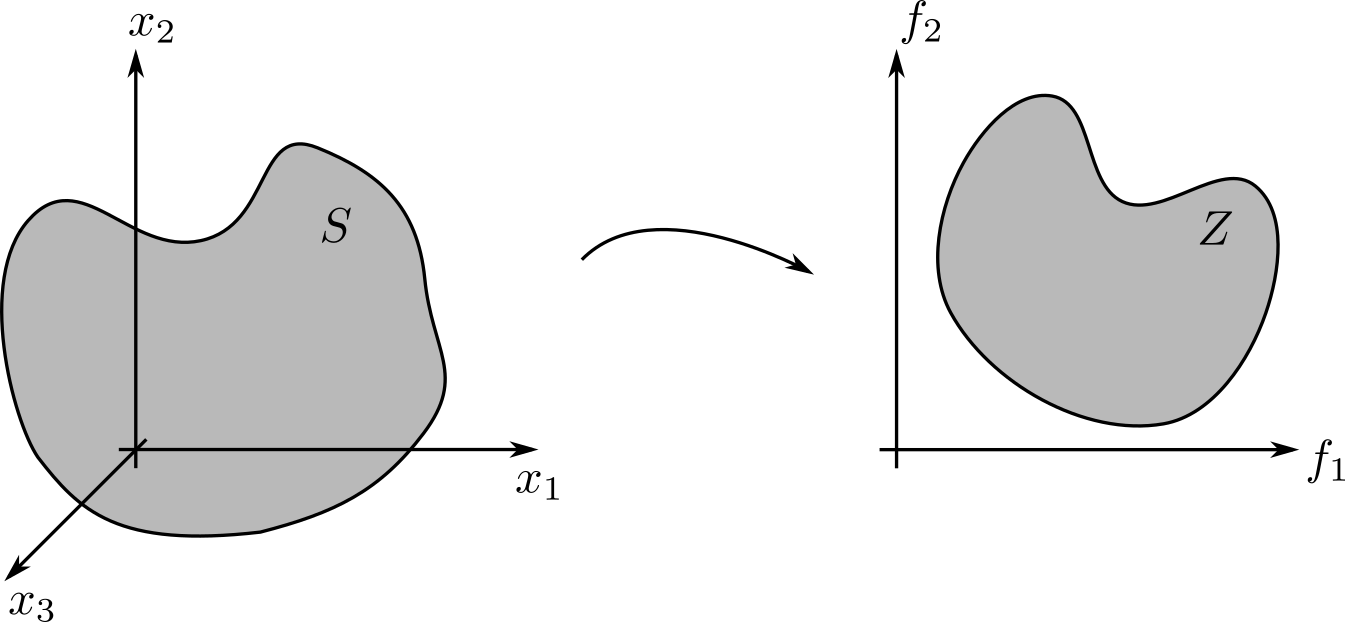
\includegraphics[width=0.6\textwidth]{Figures/2/searchSpaceFunction.png}
        \caption{Search ($S$) and function ($Z$) space in multi-objective optimization}
        \label{fig:twoSpaces}
    \end{figure}    
    
    A visual example of this kind of problems can be seen in Figure \ref{fig:BihnKorn}, where the test function proposed by Binh and Korn (Test Case 2 from \cite{binh1997mobes}) is plotted. The function was stated as:
    \begin{equation}
        \begin{array}{cl}
            \textrm{minimize} & 
            \left\{ \begin{array}{l}
                f_1(x_1,x_2) = 4x_1^2 + 4x_2^2\\
                f_2(x_1,x_2) = (x_1-5)^2+(x_2-5)^2
            \end{array} \right. \\
            & \\
            \textrm{subject to} &  
            \left\{ \begin{array}{l}
                (x_1-5)^2+x_2^2-25 \leq 0\\
                -(x_1-8)^2-(x_2+3)^2 + 7.7 \leq 0
            \end{array} \right. \\
            & \\
            \textrm{bounded by} & -15 \leq x_i \leq 30, \ \ \forall i = 1,2
        \end{array}
        \label{eq:BihnKorn}
    \end{equation}
    
    \begin{figure}[h!]
        \centering
        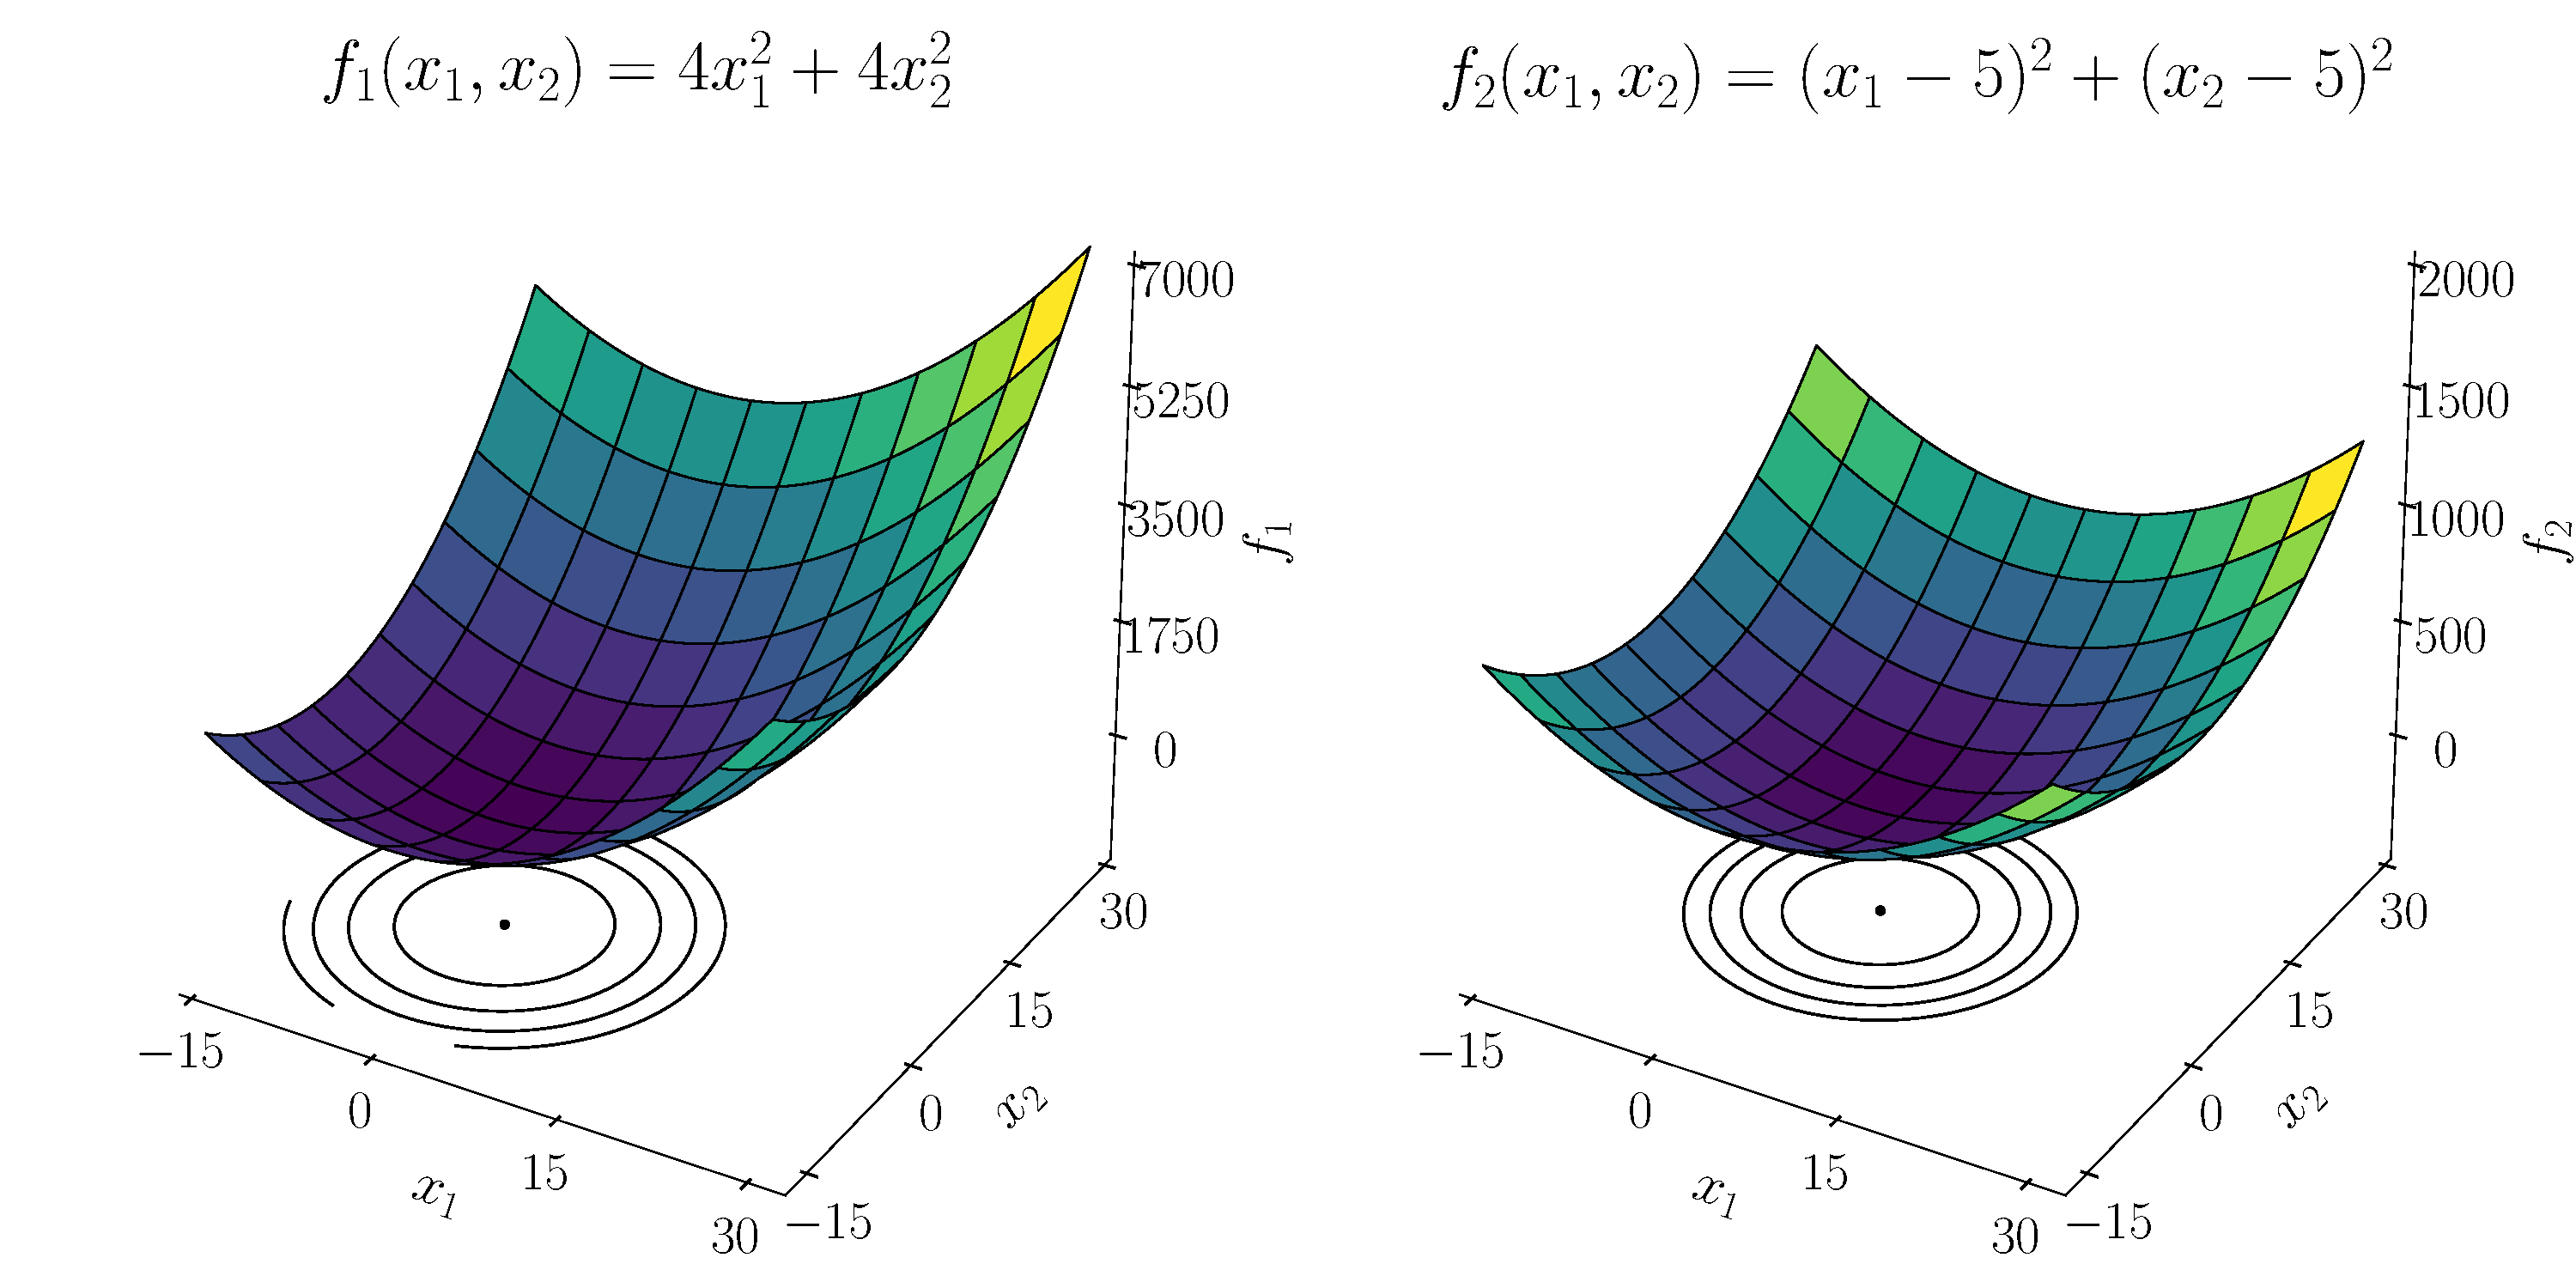
\includegraphics[width=0.8\textwidth]{Figures/2/BK2.pdf}
        \caption{Bihn and Korn test function}
        \label{fig:BihnKorn}
    \end{figure}

\newpage    
    
    As it can be seen in Figure \ref{fig:BihnKorn}, both objective functions are smooth and have defined maximums, but they are not located in the same $\bm{x}$: in the case of $f_1$ the minimum is located in $(0,0)$ and in $f_2$ the minimum is in $(5,5)$. Thus, instead of having one unique solution $\bm{x}$ a set of $\bm{x^*} \in S$ will form the \say{optimum} solution. This set of possible values will not be able to optimize both functions at the same time, having a trade-off situation. From that set of possible solutions, a decision maker should choose the best combination based on previous information. The value of $f(\bm{x^*})$ is the objective vector for the optimum decision vector $\bm{x^*}$.

\subsubsection*{Weighted averaged sum}

    The problem of optimizing multiple objectives at the same time may seem banal: transforming the multi-criteria problem into a weighted sum of the different objective functions is one approach that has been widely used and developed (see \cite{stanimirovic2011linear} and \cite{kim2006adaptive}). This plain aggregating approach consists of:
    
    \begin{equation}
        \begin{array}{cl}
            \textrm{minimize} & F(\bm{x}) = \displaystyle \sum_{m=1}^{k}  w_m f_m(\bm{x}) \\
            \textrm{subject to} & \bm{x} \in S
        \end{array}
        \label{eq:weightedSum}
    \end{equation}
    
    
    This may seem like a good approach. Its main advantage is the simplicity, but the success of the method largely depends on the chosen weights, which value is determined by the relative importance of each objective to the additive objective. It has also problems when dealing with non-convex objective spaces, given that some solutions can't be represented with the average sum \cite{jakob2014pareto}, \cite{fonseca1995overview}.

\subsection{Pareto front}

    When there are multiple functions that are to be minimized with a trade-off between them that doesn't allow the existence of a single optimum decision vector $\bm{x}$, Pareto dominance concept arises. Let's assume that there are two feasible solutions that belong to the search space, such that $\bm{x}^1\in S$ and $\bm{x}^2\in S$. 
    
    \newpage
    
    It is said that the solution $\bm{x}^1$ dominates the solution $\bm{x}^2$ when $\bm{x}^1 \prec \bm{x}^2$. The formal definition of the Pareto dominance between two decision vectors is \cite{collette2013multiobjective}:
    
    \begin{equation}
        \bm{x}^1 \prec \bm{x}^2\ \ \ \textrm{if} \ \ \left\{
        \begin{array}{rl}
            f_i(\bm{x}^1) \leq f_i(\bm{x}^2)&  \forall i \in \{1,2,3,...,k\}\\
            f_j(\bm{x}^1) < f_j(\bm{x}^2) & \textrm{for at least one } j \in \{1,2,3,...,k\} 
        \end{array} \right.
        \label{eq:ParetoDominance}
    \end{equation}
    
    The concept of Pareto dominance is shown with a graphical explanation (restricted for 2 objective problems for simplicity) in the next figure:
    
    \begin{figure}[h!]
        \centering
        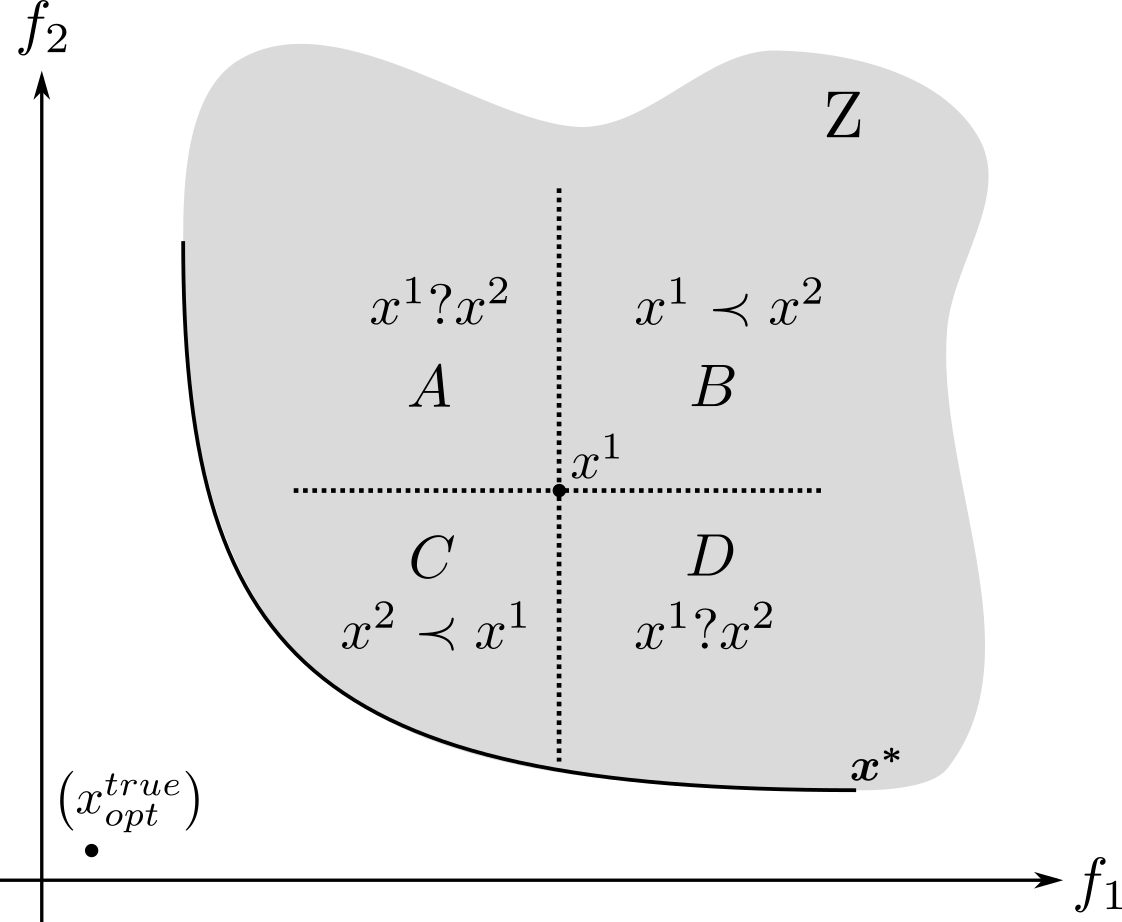
\includegraphics[width=0.75\textwidth]{Figures/2/paretoFront4cuad.png}
        \caption{Pareto front dominance concept example}
        \label{fig:4cuad}
    \end{figure}
    
    Each decision vector $\bm{x}^1$ splits the function space in 4 areas. A decision vector $\bm{x}^2$ (assuming that $\bm{x}^1 \neq \bm{x}^2$) may belong to:
    \begin{itemize}
        \item \textit{Area A} or \textit{Area D}: the relation between $\bm{x}^1$ and $\bm{x}^2$ cannot be determined, given that one performs better in one objective but worse in the other and viceversa.
        \item \textit{Area B}: there is a Pareto dominance relation, having $\bm{x}^1 \prec \bm{x}^2$, where vector $\bm{x}^1$ dominates $\bm{x}^2$.
        \item \textit{Area C}: there is also a Pareto relation between the decision vectors, having $\bm{x}^2 \prec \bm{x}^1$. Thus, $\bm{x}^1$ is dominated by $\bm{x}^2$.
    \end{itemize}
    
    \newpage
    
    If there is one decision vector $\bm{x}^*$ for which there is not any other $\bm{x}$ in \textit{Area C} (i.e. there is not any solution that dominates $\bm{x}^*$) it is said that it is Pareto optimal or non-dominated. The set of Pareto optimal solutions $(\bm{x}^*)$ is usually called Pareto front or Pareto frontier, which consists of all non-dominated decision vectors (Figure \ref{fig:4cuad}). It can also be seen which is the \say{true} optimum value, although given that it is outside the function space $Z$ it is not a valid solution.
    
    The representation of the Pareto front in optimization problems with just two objectives is quite straightforward, as seen in Figure \ref{fig:4cuad}. The Pareto front can be also represented in three dimensions with surfaces, but in high-order multi-objective optimization cases, the representation becomes harder. For those problems, there are other alternatives to the classical representation, e.g. slices of the Pareto front \cite{jaini2017fuzzy}, \cite{triantaphyllou2000multi}. One typical approach consists of Interactive Decision Maps (IDM) that are techniques that use the concept of the Edgeworth box to show the feasible set expanded by the decision vectors dominated by it \cite{lotov2013interactive}.
    
    Although the optimization process has been described to minimize functions (changing $f_i$ to$-f_i$ in  case it must be maximized), with the Pareto front all possible combinations of maximization and minimization may be analyzed, as seen in Figure \ref{fig:maxmaxminmin}, where depending on the optimization type used, a different zone of the function space is chosen as Pareto front \cite{deb2001multi}:
    \begin{figure}[h!]
        \centering
        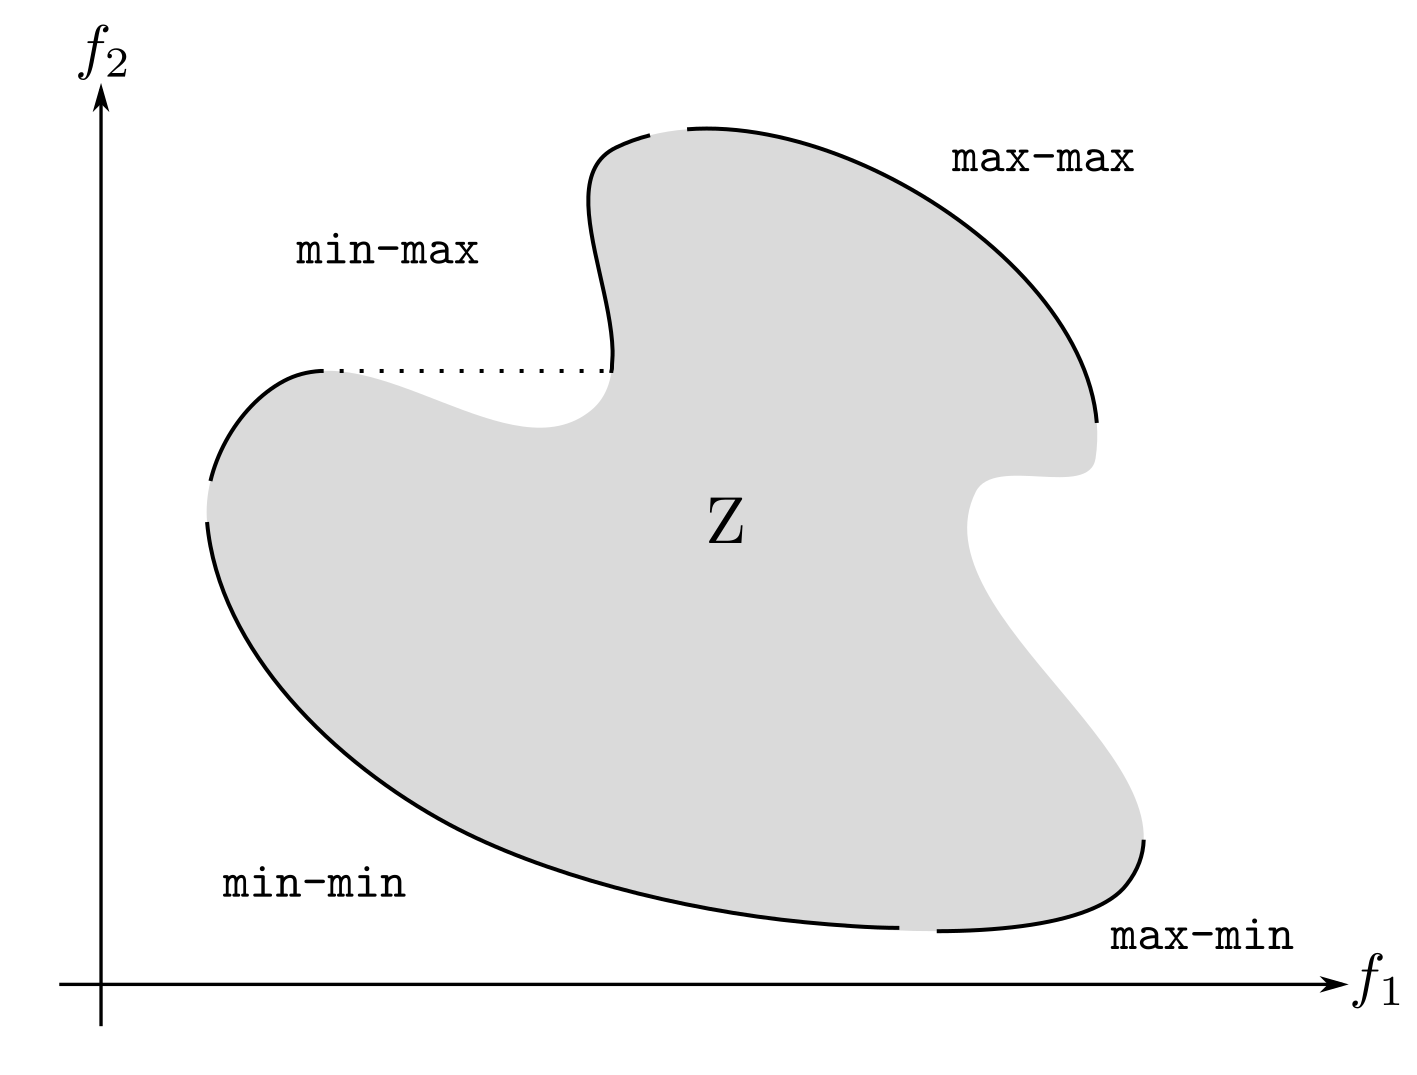
\includegraphics[width=0.75\textwidth]{Figures/2/maxmaxminmin.png}
        \caption{Different Pareto front depending on the type of optimization}
        \label{fig:maxmaxminmin}
    \end{figure}
    
\newpage

\subsection{Approaches for multi-objective optimization}
    One way to solve this kind of multi-objective problems is to create a random set of decision vectors to analyze the whole search space the best possible \cite{li2012momcmc}. The most widely known stochastic techniques are the MCMC (Markov Chain Monte Carlo) methods \cite{spall2005introduction}. They consist of different algorithms such as the Metropolis-Hasting algorithm \cite{altekar2004parallel} or Gibbs sampling \cite{gilks1992adaptive}. MCMC methods provide a fairly good performance with low chance of the worst case performance. As stated by the name, the methods are based on the union of two different techniques \cite{cleverAlgorithms}:
    \begin{itemize}
        \item Monte Carlo methods: they have been traditionally used in statistical physics, they are based on a random sample of the search domain, the deterministic evaluation of the inputs and the aggregation of the results.
        \item Markov chain processes: they provide a probabilistic model for state transitions or moves inside a domain. It is only dependant on the current position to determine the next position, i.e., it has no history retaining. 
    \end{itemize}
    
    Given that error in Monte Carlo methods is reduced $\propto 1/\sqrt{N}$ \cite{caflisch1998monte}, the number of evaluations in order to achieve a good accuracy must be high enough. Thus, the computational resources required to perform an analysis of this kind are considerably high if the number of search space variables is large.
    
    Other methods of solving this problem consist on physics-inspired algorithms (such as the Chaotic Optimization Algorithm), geography inspired algorithms (as the Imperialistic Competition Algorithm) and social culture inspired algorithms (such as  Memetic Algorithm or the Selfish Gene Algorithm) \cite{cui2017multi}. However, the most popular methods are the biology-inspired algorithms such as evolution based algorithms and swarm-based algorithms, which will be discussed in the following section.

\newpage

\section{Evolutionary computation}

    Talking about artificial intelligence (AI) and machine learning may seem unrelated to the previous topic at first, but given that evolutionary computation is a sub-field of it, both must be introduced in order to know how it is structured. Artificial intelligence is a cross-disciplinary field that combines the understanding of the brain from neuroscience, the rise of computers and the new mathematics of information and control theory \cite{cleverAlgorithms}. Therefore, AI is related to the development and investigation of systems that act in an intelligent way. Machine learning is the study of learning processes in different manifestations, i.e. machine learning is another subdivision of artificial intelligence which is focused on problem-solving \cite{michalski2013machine}.
    
    Inside artificial intelligence there are different sub-disciplines, not limited to the ones shown in the next summary: 
    \begin{itemize}
        \item Evolutionary computation: systems based on the Darwinian theory of evolution built on the natural selection of the better genes. There are different kinds of algorithms such as:
            \begin{itemize}
                \item Genetic algorithms: it is a global optimization method with an adaptive strategy. It is based on the understanding of the structure and mechanisms of the genetics.
                \item Genetic programming: it consists of the same principles of genetic algorithms but applied to computer software that adapts and improves the code over time. Instead of coding the lines with the instructions to perform certain tasks, the task is imposed and the evolutionary computation gets the optimum code to perform that task \cite{koza2006genetic} (even improving human coded programs \cite{cramer1985representation}).
                \item Differential evolution: following the same principles as any other evolutionary computation, in this case, a scaled difference mutation is used instead of the typical probability distribution. It is usually used from constrained, large-scale and uncertain optimization problems, as well as multiobjective problems with multiple variables \cite{das2011differential}.
            \end{itemize}
        \item Swarm intelligence: systems based on a large number of not-very-wise individuals that cooperate and interact with each other, obtaining as result a collective intelligence.
        \newpage
        \item Artificial neural networks: systems that are based on a network that behaves as the neurons in the brain: managing the feedback from the environment and achieving some adaptive learning with it.
        \item Fuzzy intelligence: systems that consider a logic with degrees of truth instead of the constrained duality of true and false \cite{klir1996fuzzy}.
    \end{itemize}
    
    
    The classical AI field is divided into two approaches to the problems: \textit{neat AI} and \textit{scruffy AI}. The former uses symbolic representations and logic processes to analyze the given problem, achieving high fidelity in the results. The reductionist analysis is translated into scalability limits: a small increment in the size of the problem leads to an unmanageable increase in the complexity of the system (exaggerated execution time or computing resources). The latter is a descriptive method that takes advantage of the complex, emergent and self-organizing behavior of simple procedures. Using inductive approaches and some stochasticity in the system, the process is more robust when trying to approximate the solution of intractable problems with other methods. Scruffy AI is also known as \textit{metaheuristic}: where \textit{meta-} refers to the higher level strategy of combining different methods or procedures and \textit{-heuristic} is the method that, in order to achieve faster computation time and less resource consuming processes, reduces the precision and quality of the solution (keeping it accurate enough to be sufficient for the case requisites) . These heuristic methods are approximate (global solution cannot be ensured), normally non-deterministic and not problem-specific \cite{cleverAlgorithms}.
 
    Conventional algorithms to approach optimization problems (not restricted to multi-objective optimization) are varied: Newton's method, Gradient Descent, Simplex method, Nelder-Mead method,... Besides all these well-known techniques, there are algorithms that do not exploit information given from the problem to obtain a solution. This group is usually named as black-box optimization and it includes methods as genetic algorithms (given that only an evaluation of a decision vector is required). These techniques may be applied to a wide range of different problems with small modifications in the algorithm \cite{droste2006upper}. Associated with these black-box algorithms, the \textit{no-free-lunch} theorem states that if one algorithm performs better than other in one particular case, that offset will be reversed for other problems where it will perform worse \cite{wolpert1997no}. This proposition caused pessimism when comparing different optimization techniques, but it can be understood as if each problem is most suitable to certain algorithm that may not be valid for other cases - having to choose the better algorithm for each situation.

\newpage

\subsection{Genetic algorithms overview}
    
    A genetic algorithm (shortened as GA) is a population-based technique that tries to search for solutions to certain problems instead of searching paths for goals. Although searching one solution includes searching the path to achieving that solution, the main target of the algorithm is searching a solution in a large space efficiently instead of developing a decision tree to achieve a goal in all situations \cite{mitchell1998introduction}.
    
    Given that genetic algorithms are based on biological evolution, some biological terminology may be used in the discussion (although mathematical terminology will take precedence). Therefore, before going into the details, these basic terms will be introduced. Cells are the basic element of all living organism and they store the DNA string structured in chromosomes. Each chromosome is divided into genes located in a particular locus of the chromosome, encoding each one gene for a protein. Most parts of the organisms have more than one chromosome per cell. All those possible chromosomes form the genome of the individuals, having that all genes contained inside a genome form the genotype of an organism. 

    There is a close relationship between optimization and genetic algorithms - that is why GA are such a good approach to optimization problems. As it has been mentioned (Figure \ref{fig:twoSpaces}), optimization used two different spaces: parameter space ($\bm{x}$) and function space ($f(\bm{x})$). In genetic algorithms, there are also two spaces that represent the same concept: \textit{search} space and \textit{fitness} landscape. The search space is the set of all possible states that certain individual or chromosome may have (having each one different genes or components). Fitness landscape is the representation of all possible genotypes with their fitness. The fitness of an individual is a representation of \say{how good} its chromosome is inside the population, which is translated into the possibilities of having offspring. Genetic algorithms assume that individuals with high fitness will have offspring that will have high fitness too - and it is there where the capabilities of GA relies on.
    
    One aspect that makes genetic algorithms a very broad topic are the two possible ways of encoding the chromosome of each individual: \textit{binary} and \textit{real-valued} (although others as tree encoding or permutation encoding \cite{ronald1995genetic} have been also proposed). Binary encoding is the most common encoding, for both historical reasons and simplicity when dealing with the different operators. However, coding a state with strings of 0 and 1 when dealing with real numbers is unwieldy. In those cases, a real-valued encoding is preferred. This encoding is not limited to the use of float number but also strings of numbers, even combined with letters. The versatility of this encoding makes it widely used and the chosen one for further analysis. 
    
\subsection{Structure of a simple genetic algorithm}
    
    The main operation of a genetic algorithm and its structure will be described in this subsection. A genetic algorithm begins with the initialization of a population. It may be done in a random way, in an equally spaced way or in any other type of sampling of the search space. The \textit{fitness} of the population is evaluated according to the function and objectives selected. Each individual of the population will have a fitness value associated. Then  the three \textit{genetic algorithm operators} are applied:
    
    \begin{itemize}
        \item Selection: this operator selects individuals from the population. There are different types of selection, but the two more common ones are \cite{zhong2005comparison}:
        \begin{itemize}
            \item Roulette wheel selection: random individuals are chosen according to a probability proportional to the fitness value that each individual has.
            \item Tournament method: $n$ uniformly random chosen individuals are faced in a tournament, selecting the one with higher fitness.
        \end{itemize}
        Any selection operator must ensure that the fitter the chromosome, the more times it is selected.
        \item Recombination: two individuals are chosen from the ones selected and are combined, giving rise to (at least) one new individual. As it has already been pointed out, GA assumes that the higher the fitness of the parents, so will be the fitness of the offspring. Recombination tries to increase convergence of the system by joining together points with high fitness. In this recombination phase, there are three possibilities that may exist \cite{thevenin2008and}:
        \begin{itemize}
            \item Crossover: some of the genes are taken from one parent and the rest of the genes of the offspring chromosome are taken from the other parent. It is used to increase the diversity.
            \item Average: two parents are chosen and create the chromosome of the offspring with the mean value of each of its genes. This may also be a weighted sum of the parents instead of a plain 50-50 mean.
            \item Survival: it is not exactly recombination but the survival of one of the two chromosomes of the parents. This method takes the chromosome of a parent and saves it in the offspring population. Survival is also known as elitism, given that the elite of the population (sorted by the fitness value) will be preserved along generations.
        \end{itemize}
        \item Mutation: perturbations are applied to each individual in order to ensure variability. The probability of mutation is usually chosen as input, with a value different from zero. The task of mutation is to introduce diversity back into the population. In optimization, this has an especial meaning, given that the GA must move between different optimum locations to analyze the whole domain, so it must be able to leave a local minimum in case it gets stuck in one. Mutation can be applied to a whole chromosome or only to some of its genes. It is a random process, so individuals may not be mutated and keep the chromosomes obtained after recombination.
    \end{itemize}
    
    \begin{figure}[h!]
        \centering
        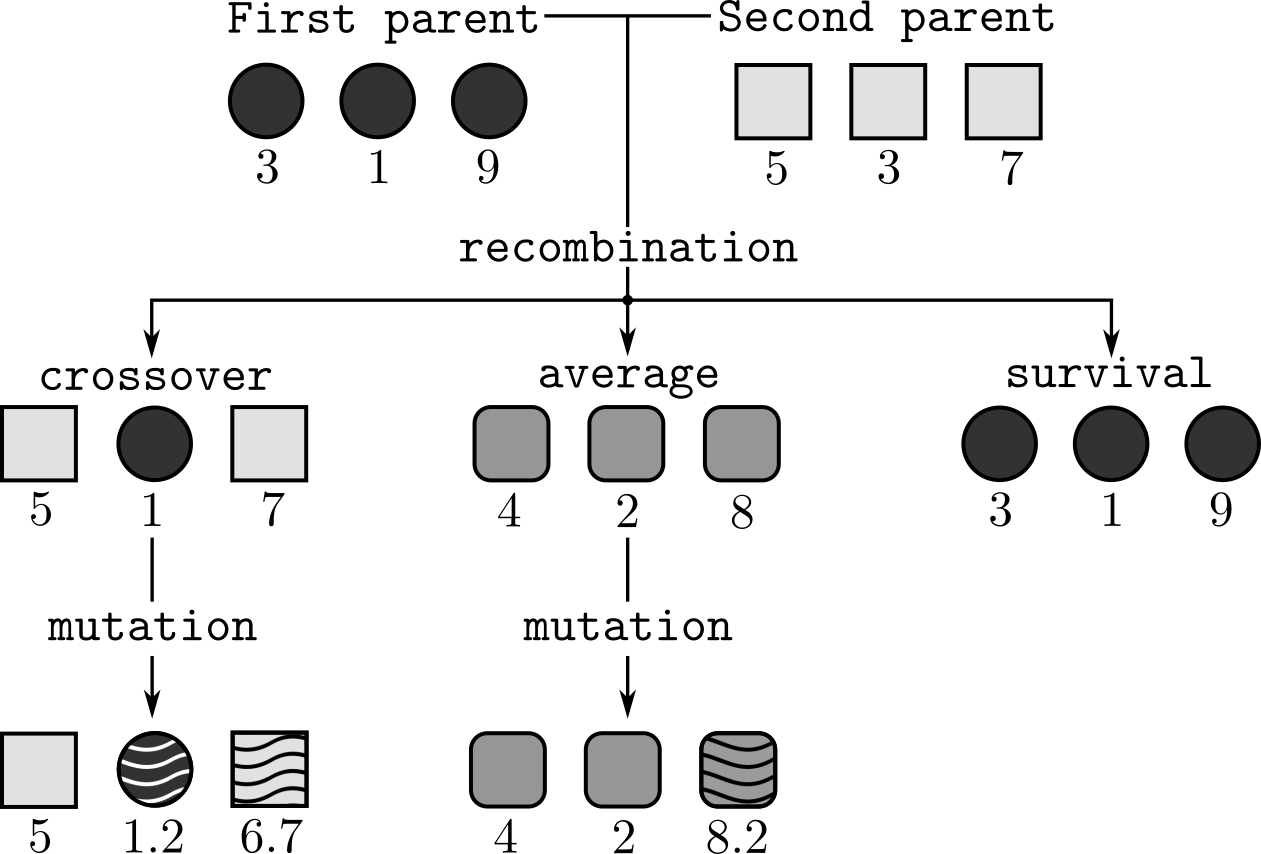
\includegraphics[width=0.8\textwidth]{Figures/2/crossover.png}
        \caption{Recombination and mutation process from two parents}
        \label{fig:crossoverTheory}
    \end{figure}

    Once these three operators have been applied, a new population will arise - having a new generation. That population will undergo the same cycle until one stop condition is matched: it is usually the maximum number of generations or some relative error. For each generation two basic groups must exist: \textit{parents} (individuals that have been chosen to reproduce) and \textit{offspring} (individuals obtained from the combination of the parents). A third group, \textit{elite}, may exist if the genetic algorithm applies the survival operator. Elitism \cite{yager2012introduction} has been proved to have a considerable impact on performance, because it avoids wasting time in discovering again zones that have been already discarded as not valid. The same individual may be part of several groups at the same time, i.e. there are algorithms that compare the value of parents and offspring to keep the better for recombination and mutation.

    \newpage
    
    Genetic algorithms may be mathematically formalized for simple cases (see \cite{goldberg2006genetic}, \cite{vose1991punctuated}, \cite{whitley1993executable}), being able to analyze the dynamics of the system. GA are used for optimization problems, where once the optimum value is found, the state does not move from there. This kind of points are fixed points and, in genetic algorithms, they are achieved once a population has completely converged to individuals with the same (maximum) fitness. If a population does not have all individuals at the maximum fitness level, a small perturbation may move the solution from the fixed point. This situation causes \textit{punctuated equilibrium} in fitness evolution: long periods of no improvement with quick rises in the fitness. Although these effects have to be rigorously quantified under different models, the implications are that a large enough number of generations must be computed to achieve a high fitness. The main assumption in the mathematical formulation is that the population has an infinite size, which may lead to unexpected behaviors due to sampling errors when comparing with a real genetic algorithm with a limited population size. 
    
    The basic procedure of a genetic algorithm is listed below:
    \begin{algorithm}
        \caption{Simple Genetic Algorithm}\label{alg:simpleGApseudoCode}
        \begin{algorithmic}[1]
        \State initialize \textit{population}
        \While {stopCriterion \textbf{not} reached }
            \State calculate \textit{fitness} of \textit{population}
            \State select \textit{bestIndividuals} from \textit{population}
            \State \textit{newPopulation} $\leftarrow$ mutation $\leftarrow$ crossover \textit{bestIndividuals}
            \State \textit{population} $\leftarrow$ \textit{newPopulation}
        \EndWhile
        \end{algorithmic}
    \end{algorithm}

\subsection{Why do genetic algorithms work?}

    Although a genetic algorithm is procedure simple to describe and code, its behavior may be complicated and there are still many questions about how do they really work. A genetic algorithm results in complex and robust search method by implicitly sampling hyperplane partitions of a search space \cite{whitley1994genetic}.
    The genetic algorithm works by discovering and recombining good \textit{building blocks} of solutions, given that a good building block will make up a good building block.
    Holland's book \cite{john1992holland} refers to this building blocks as \textit{schemas} that defines hyperplanes. One schema on its own does not provide enough information, that is where the population-based search concept is critical, given that many hyperplanes are evaluated at the same time. The cumulative effects of evaluating a population of points will provide enough information about any particular subset of hyperplanes.

\newpage

\subsection{Genetic algorithms for multi-objective optimization}
        
    Due to the similarities between genetic algorithms and multiobjective optimization, there are a lot of existing and well-tested methods that combine both. The ability of a GA to search in different regions of the solution space in a highly parallel fashion makes it a good tool for problems with non-convex, discontinuous and multi-modal solution spaces. Undoubtedly, genetic algorithms are one of the most popular heuristic approaches to multi-objective optimization. 
    In the next table, the most popular genetic algorithms and some of its special features are listed \cite{konak2006multi}:
    \begin{table}[H]
    \centering
    \caption{Different genetic algorithms for multi-objective optimization}
    \begin{tabular}{lllcc} 
    \hline
    \textbf{Algorithm} & \textbf{Fitness assignment} & \textbf{\begin{tabular}[c]{@{}l@{}}Diversity~\\mechanism\end{tabular}} & \textbf{Elitism} & \textbf{\begin{tabular}[c]{@{}l@{}}External~\\population\end{tabular}} \\ 
    \hline
    VEGA & \begin{tabular}[c]{@{}l@{}}Each population is~\\evaluated with respect~\\to a different objective\end{tabular} & No & No & No \\ 
    \hline
    MOGA & Pareto ranking & \begin{tabular}[c]{@{}l@{}}Fitness sharing ~\\ by niching\end{tabular} & No & No \\ 
    \hline
    PESA & No fitness assignment & Cell-based density & Yes & Yes \\ 
    \hline
    NSGA & \begin{tabular}[c]{@{}l@{}}Ranking based on~\\non-domination sorting\end{tabular} & Niching & No & No \\ 
    \hline
    NSGA-II & \begin{tabular}[c]{@{}l@{}}Ranking based on~\\non-domination sorting\end{tabular} & Crowding distance & Yes & No \\ 
    \hline
    SPEA &  \begin{tabular}[c]{@{}l@{}}Ranking based ~\\ on external archive ~\\ of non-dominated \end{tabular} & \begin{tabular}[c]{@{}l@{}}Clustering to ~\\ truncate external ~\\ population\end{tabular} & Yes & Yes \\ 
    \hline 
    SPEA-2 & Strength of dominators & \begin{tabular}[c]{@{}l@{}}Density based of~\\ $k$ nearest\end{tabular} & Yes & Yes \\ 
    \hline 
    DMOEA & Cell-based ranking & \begin{tabular}[c]{@{}l@{}}Cell-based~\\density\end{tabular} & Yes & No \\
    \hline
    \end{tabular}
    \label{table:differentMOGA}
    \end{table}
    Many other genetic algorithms exist and have been also tested, but only the most common have been listed above. There are some nomenclature that may have not been introduced and it must be explained before analyzing the advantages and disadvantages of each method:
    \begin{itemize}[label={--}]
        \item \textbf{Fitness assignment}: procedure followed to assign a value (\textit{fitness}) for every individual that shows \say{how good} does it perform in the population.
        \item \textbf{Diversity mechanism}: techniques used to promote the diversity of the solutions, i.e., the spread of individuals to cover the whole search and function space.        

        \newpage

        \item \textbf{Elitism}: for a single-objective genetic algorithm, elitism consists on saving the best solution for the next generation. However, in multi-objective optimization, all non-dominated solutions that form the Pareto front are considered elite solutions but elitism is not as straightforward as in single objective. Although earlier genetic algorithms did not include elitism, most recent strategies include it because it outperforms non-elitist counterparts.
        \item \textbf{External population}: proposes to save in a list the elitist individuals for each generation. Apart from being a computationally expensive task, the size of the list may grow too much. In order to avoid that, pruning techniques have been proposed to limit the maximum size of the elitist population.
        \item \textbf{Fitness sharing}: a method used to encourage the search in unexplored zones of a Pareto front by artificially reducing the fitness of the solutions in densely populated areas with some penalization method.
        \item \textbf{Niching}: technique consisting of segmenting the population in disjoint sets so each member may go to different zones, in order to cover more than one local optima. It is a highly used technique to widen the whole search space in fewer generations due to the splitting of the population.
        \item \textbf{Cell-based density}: consists on dividing the objective space into $K$ cells, computing the density of each cell and assigning that value to each solution in the cell. Then, the most populated cells are penalized in a similar way as fitness sharing.
        \item \textbf{Crowding distance}: technique that eliminates the necessity of a user-defined parameter such as $\sigma_{shared}$ or the $k$-nearest neighbors. It computes the distance between the points of the Pareto front and uses that distance for the selection process.
        \item \textbf{Strength of dominators}: assignment of the fitness value according to the number of individuals that dominate each individual.
    \end{itemize}
    
    Once the terminology used in this kind of genetic algorithms is known, a brief discussion about each one of them will be held. Main advantages and disadvantages will be presented and shown, in order to decide which will be the most optimum algorithm:

    \newpage

    \begin{itemize}
        \item VEGA (Vector Evaluated Genetic Algorithm): it was the first genetic algorithm designed for multi-objective optimization. Although the easy implementation, its main disadvantage is that it tends to converge to the extreme of each objective, losing an important part of the Pareto front.
        \item MOGA (Multi-Objective Genetic Algorithm): it is a simple extension of a genetic algorithm for single objective. However, it has problems related to the niche size parameter and a slow convergence.
        \item PESA (Pareto Envelope-based Selection Algorithm): it is easier to implement and (if done correctly) it is computationally efficient. The main problem is that the performance and the success of the method depend on the cell sizes and some previous knowledge about the objective space is required.
        \item NSGA (Non-dominated Sorting Genetic Algorithm): it has an extremely fast convergence but also major problems related to the niche size parameter.
        \item NSGA-II (Non-dominated Sorting Genetic Algorithm II): efficient, well tested and single parameter ($N$) method. The main disadvantage is that the crowding distance works only in the objective space.
        \item SPEA (Strength Pareto Evolutionary Algorithm): well-tested method without any user-defined parameter for clustering. Its inconvenient is that the clustering algorithm is quite complex.
        \item SPEA-2 (Strength Pareto Evolutionary Algorithm 2): it is an improved version of the SPEA that also ensures that the extreme points of the Pareto front are preserved (in order to increase both the diversity and the convergence). The drawback of the method is that the fitness and density calculation are highly computationally expensive.
        \item DMOEA (Decomposition-based Multi-Objective Evolutionary Algorithm): it is a method that combines some efficient techniques to update cell densities and adaptative approaches to set the genetic algorithm parameters. The main downside is its complicated implementation.
    \end{itemize}
    
From this list of some of the most well-known genetic algorithms for multiobjective optimization, one will be chosen for the implementation and application to the CFD cases. There are some characteristics that must exist in the genetic algorithm in order to be used successfully in these cases.

\newpage

The desired characteristics that a GA  must have for being applied successfully to CFD cases are:
\begin{itemize}
    \item Elitism: keeping the best individuals along generations has shown that the convergence of the solution is faster and requires less number of generations. Thus, it is very important that the algorithm chosen has elitism, given that each individual fitness evaluation may last minutes (or even hours) due to the CFD simulation. 
    \item Avoid user-defined parameters: achieving the correct solution is usually directly related to the value that those parameters have, so it is interesting to choose a genetic algorithm that does not have user-defined parameters. Some of these parameters include the $k$-nearest individuals or the size of the cells when performing the fitness evaluation. 
    \item Well-tested method: an algorithm whose performance has been tested and is above certain limit when talking about convergence to a solution is preferable with respect to a newer method that has not been tested yet. 
    \item Efficient and low resources consuming: given that the computational fluid dynamics simulations will be running for long periods of time, increasing the computational resources required for evaluating the fitness and performing the different operators is not a clever way of approaching the problem.
    \item Straightforward implementation: given that the code will be implemented in Python, it is also interesting to have an algorithm whose coding may be done in a simple way and with a high level of parallelization.
\end{itemize}
Analyzing the algorithms in the table \ref{table:differentMOGA}, the one that meets all the requirements is the NSGA-II. 

\subsection{Non-dominated Sorting Genetic Algorithm II}
The algorithm that was chosen to be implemented and used in the different computer fluid setups is the NSGA-II. This algorithm was first described in \cite{deb2002fast} where the algorithm is presented as a review of the first version of the NSGA. Some characteristics that make this algorithm suitable for this study have been already mentioned. However, the potential of the algorithm lays in fitness evaluation and the way it handles the populations of parents and offspring. A combination of all these parameters is what makes this algorithm so attractive for this study. 

\newpage
The main features of the NSGA-II are:
\begin{itemize}
    \item Fast non-dominated sorting: the points of an evaluation are sorted depending on the Pareto front in which they are located on. The points in the non-dominated Pareto front will have the greater fitness possible, while the points located in other Pareto fronts will have a smaller fitness. Selection is performed based on the number of the Pareto front in which the individual is located: the higher the fitness, the less dominated the individual will be by other individuals and the greater possibilities will it have to be selected.
    \begin{figure}[h!]
        \centering
        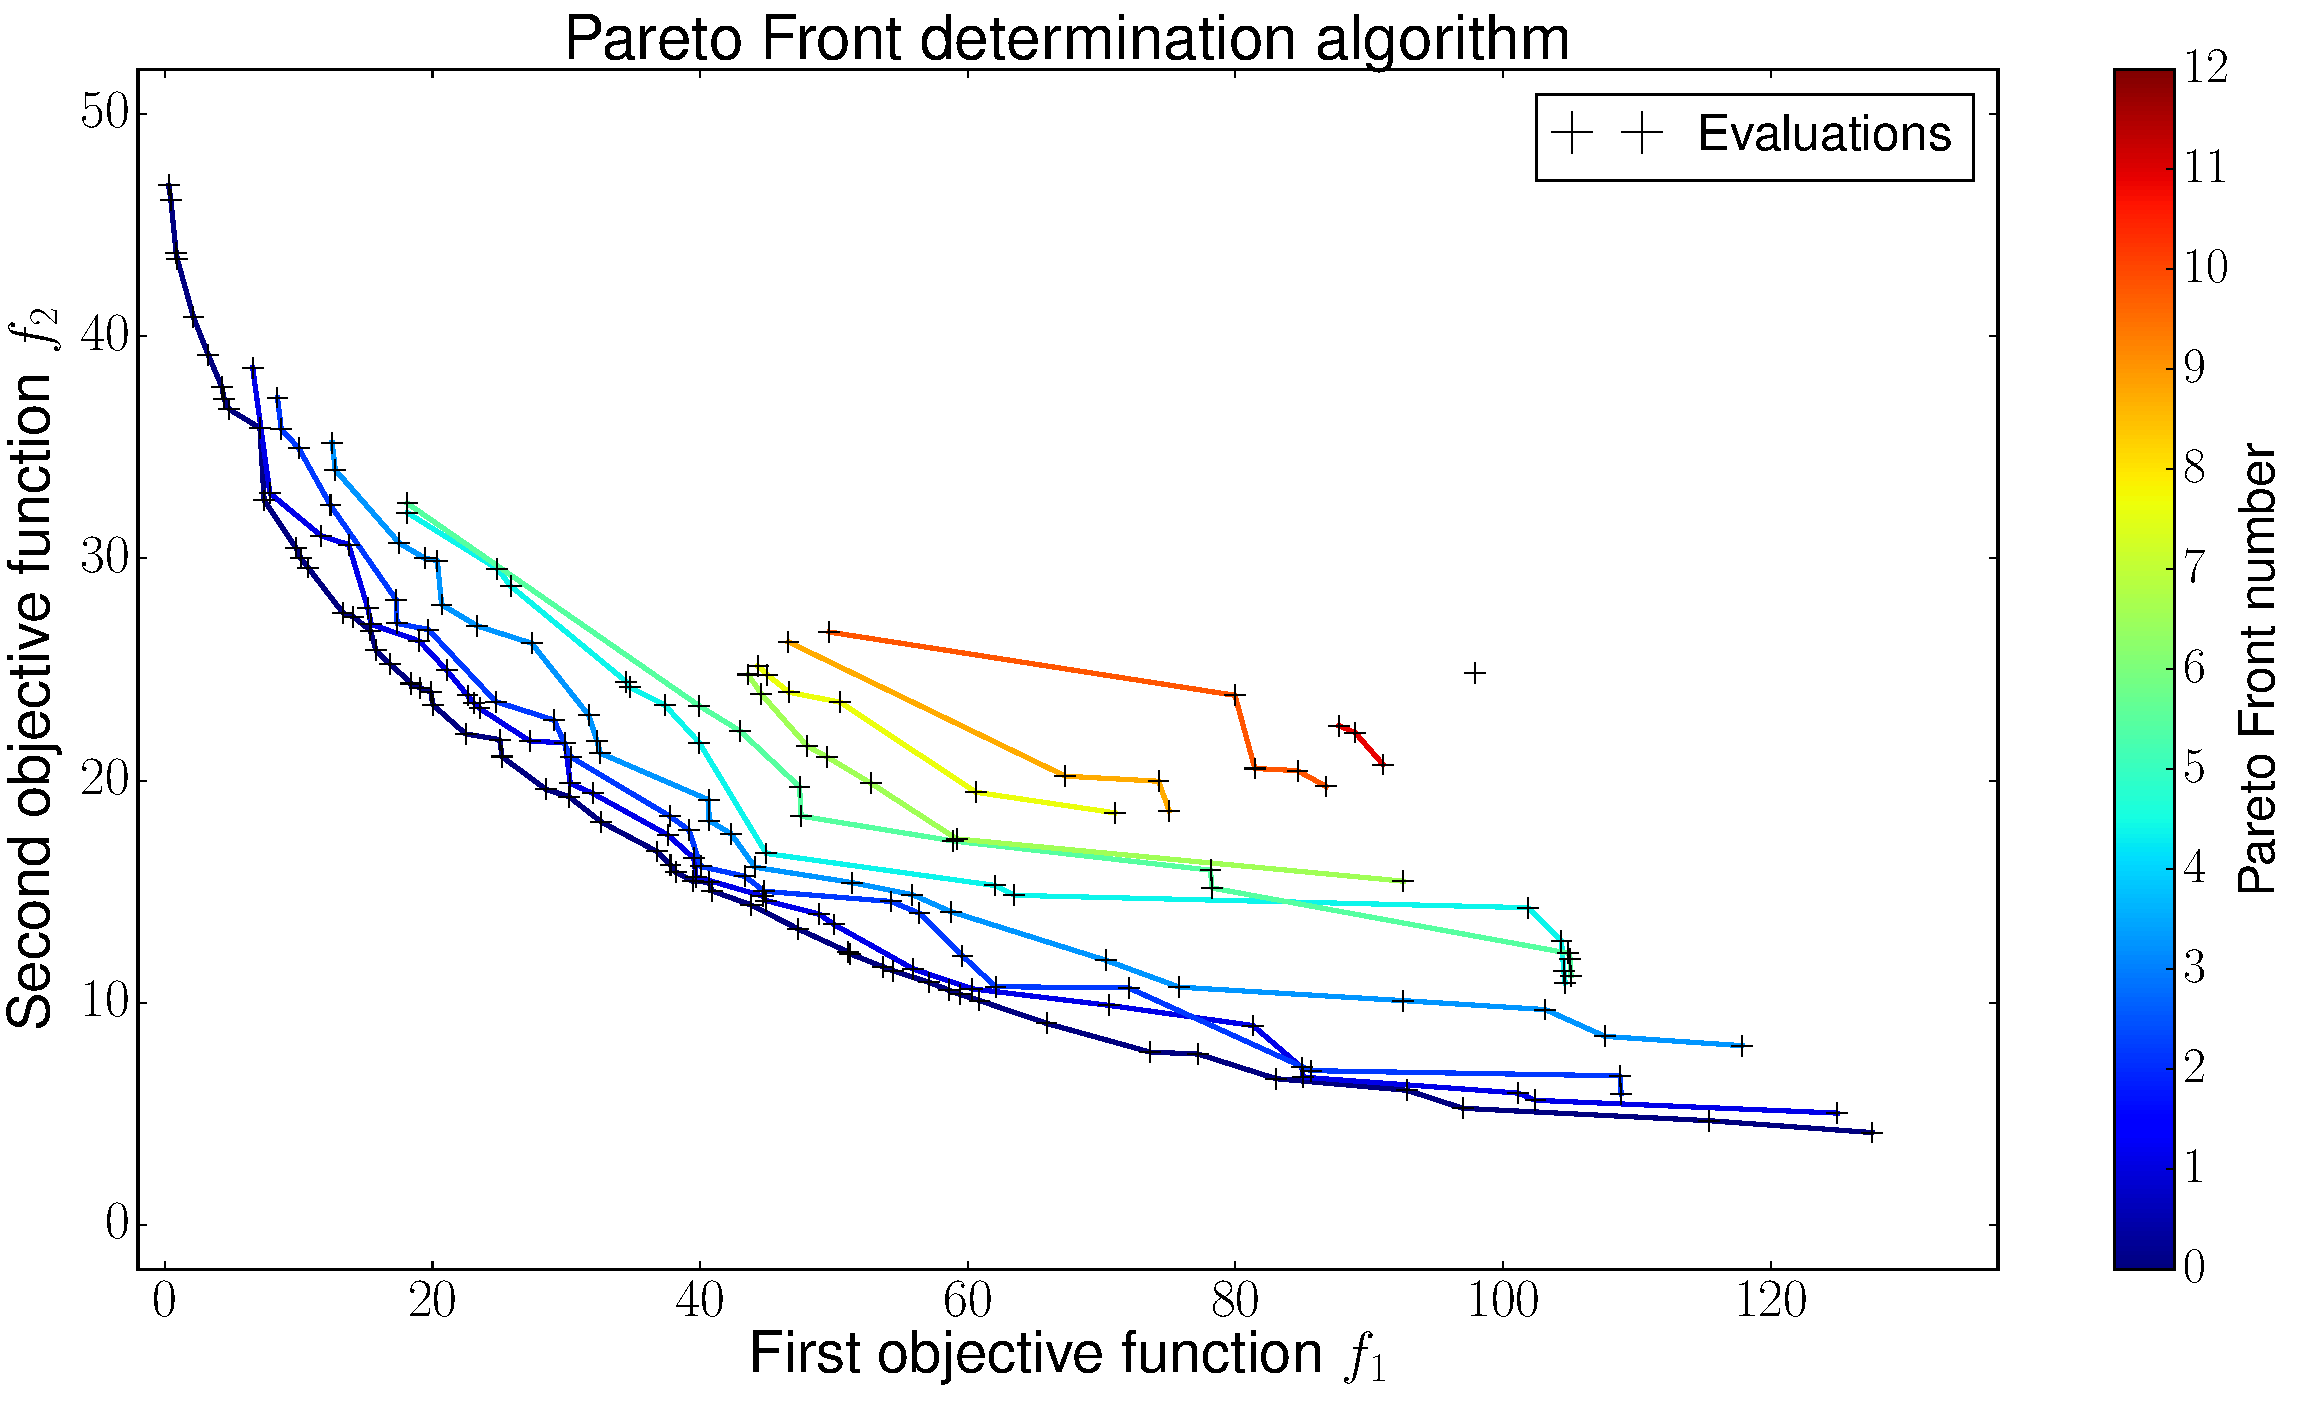
\includegraphics[width=0.85\textwidth]{Figures/2/fastNonDominatedSort.pdf}
        \caption{Fast non-dominated sorting}
        \label{fig:fast-nondominated-sorting}
    \end{figure}
    \item Crowding distance: if a selection is performed with a binary tournament ($k=2$), there are chances for two individuals of the same Pareto front to be in the tournament facing each other. Given that for the points in the same Pareto front, the value of the fitness is the same, there must exist another parameter or value used to break the tie. Crowding distance is used for that purpose, breaking possible ties in the selection process. It is assigned based on the distance to the closest point in the same Pareto front, having a higher crowding distance if the point is located in a low-density area. If the point is located in a dense area, the crowding distance will be smaller having, therefore, smaller chances of being chosen. The extrema points of the Pareto front have a crowding distance of $\infty$, so they are always chosen. In Figure \ref{fig:crowding_distance} it can be seen how points in less dense areas have a greater crowding distance.
    \begin{figure}[h!]
        \centering
        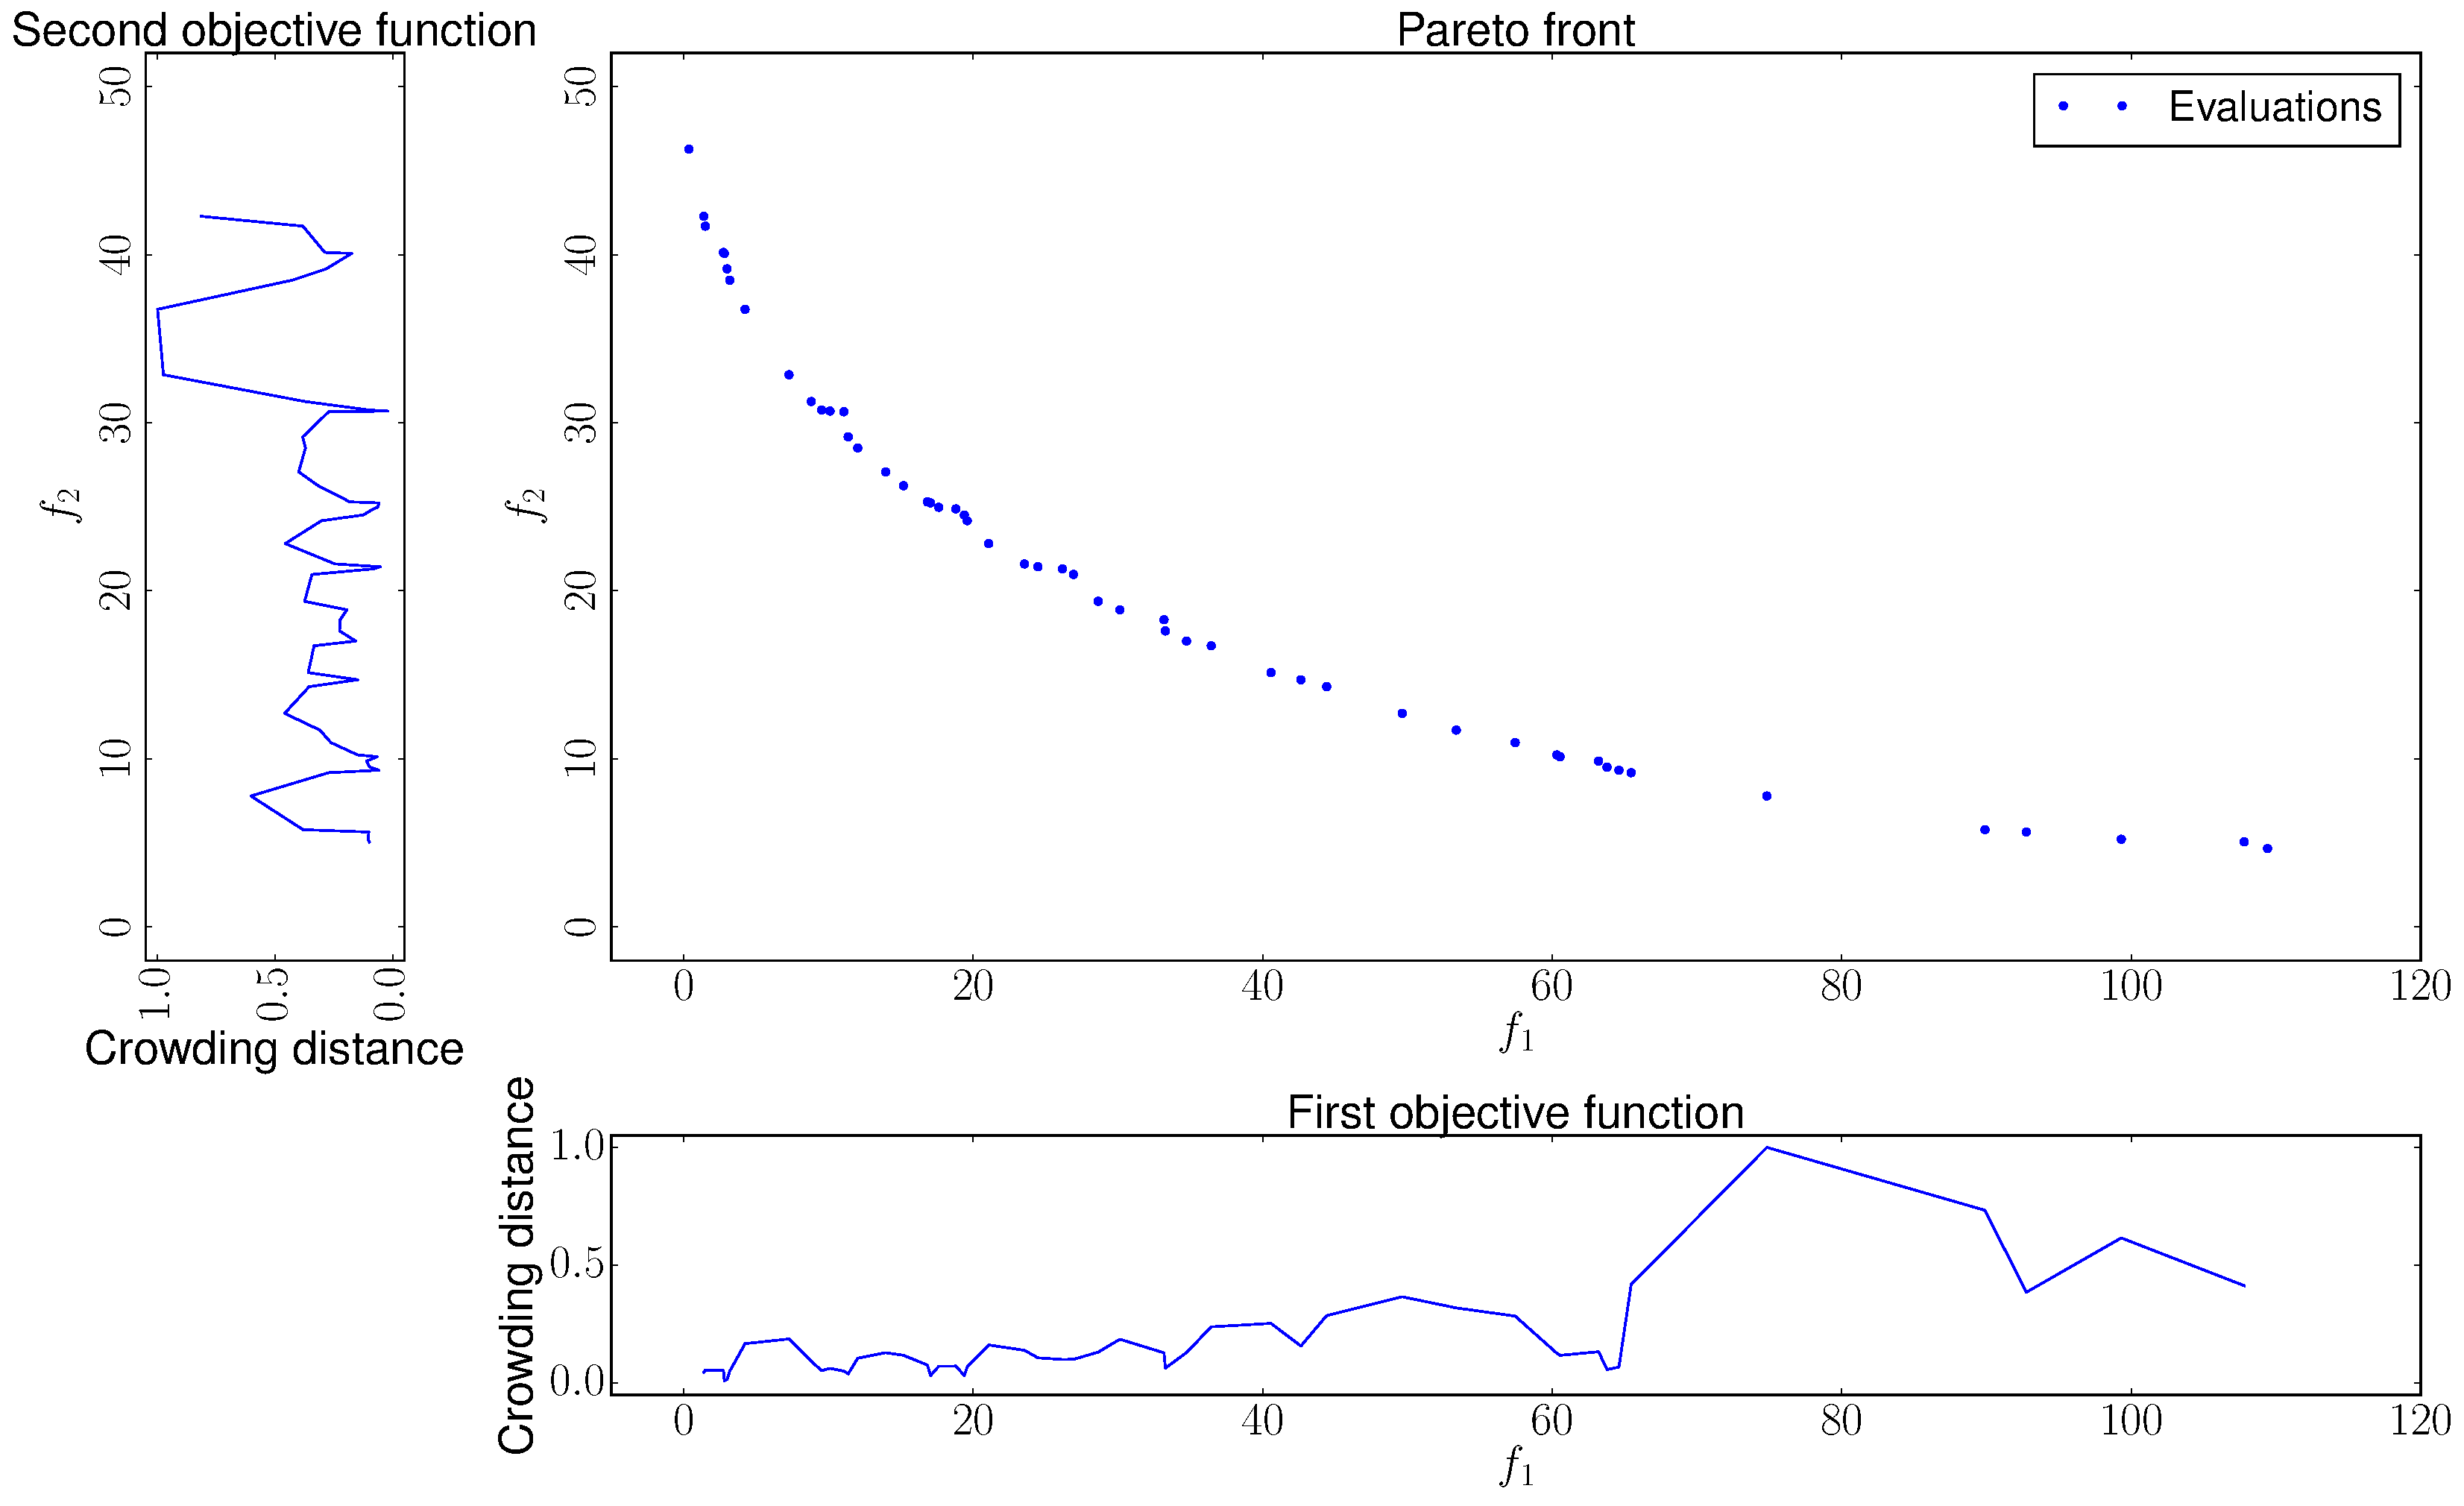
\includegraphics[width=0.95\textwidth]{Figures/2/crowdingDistance.pdf}
        \caption{Crowding distance assignment}
        \label{fig:crowding_distance}
    \end{figure}
    \newpage
    \item Preselection process: these two ways of sorting a population allow a preselection process (prior to the classical selection, recombination and mutation processes) to increase the convergence of the method. It begins with a parent population $P_t$ of size $N$ which yields an offspring population $Q_t$ of size $N$. These two populations are combined in the same set (having a size of $2N$), which is sorted according to the non-dominated sorting explained before (Figure \ref{fig:fast-nondominated-sorting}). The whole set of both parents and offspring are sorted depending on the Pareto front they are located in. Provided that the size of the new population should be $N$, the less dominated Pareto fronts that fit completely the new population will go directly without going through any other process. Once the following Pareto front will not fit completely the new population $P_{t+1}$, the set is sorted by the crowding distance. Thus, from the last Pareto front, only the points with higher crowding distance will be selected for the parent population $P_{t+1}$. The most rear fronts will not be selected for the new population as well as the lower crowding distance individuals from the last Pareto front. Those points are just rejected. Population $P_{t+1}$ will undergo selection, recombination and mutation to yield population $Q_{t+1}$, closing this way the loop. This is an indirect way of performing elitism given that the best individuals are taken from the previous generation ($P_t$).
        \begin{figure}[h!]
        \centering
        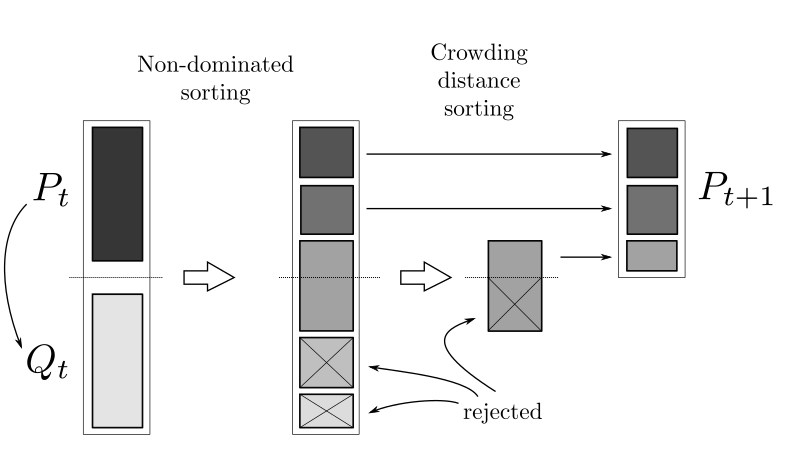
\includegraphics[width=0.9\textwidth]{Figures/2/preselection5Report.png}
        \caption{Preselection process for a parent population $P_t$}
        \label{fig:preselection process}
    \end{figure}
\end{itemize}
    
The main loop of the genetic algorithm combines all procedures shown before, having the next diagram:

\begin{figure}[h!]
        \centering
        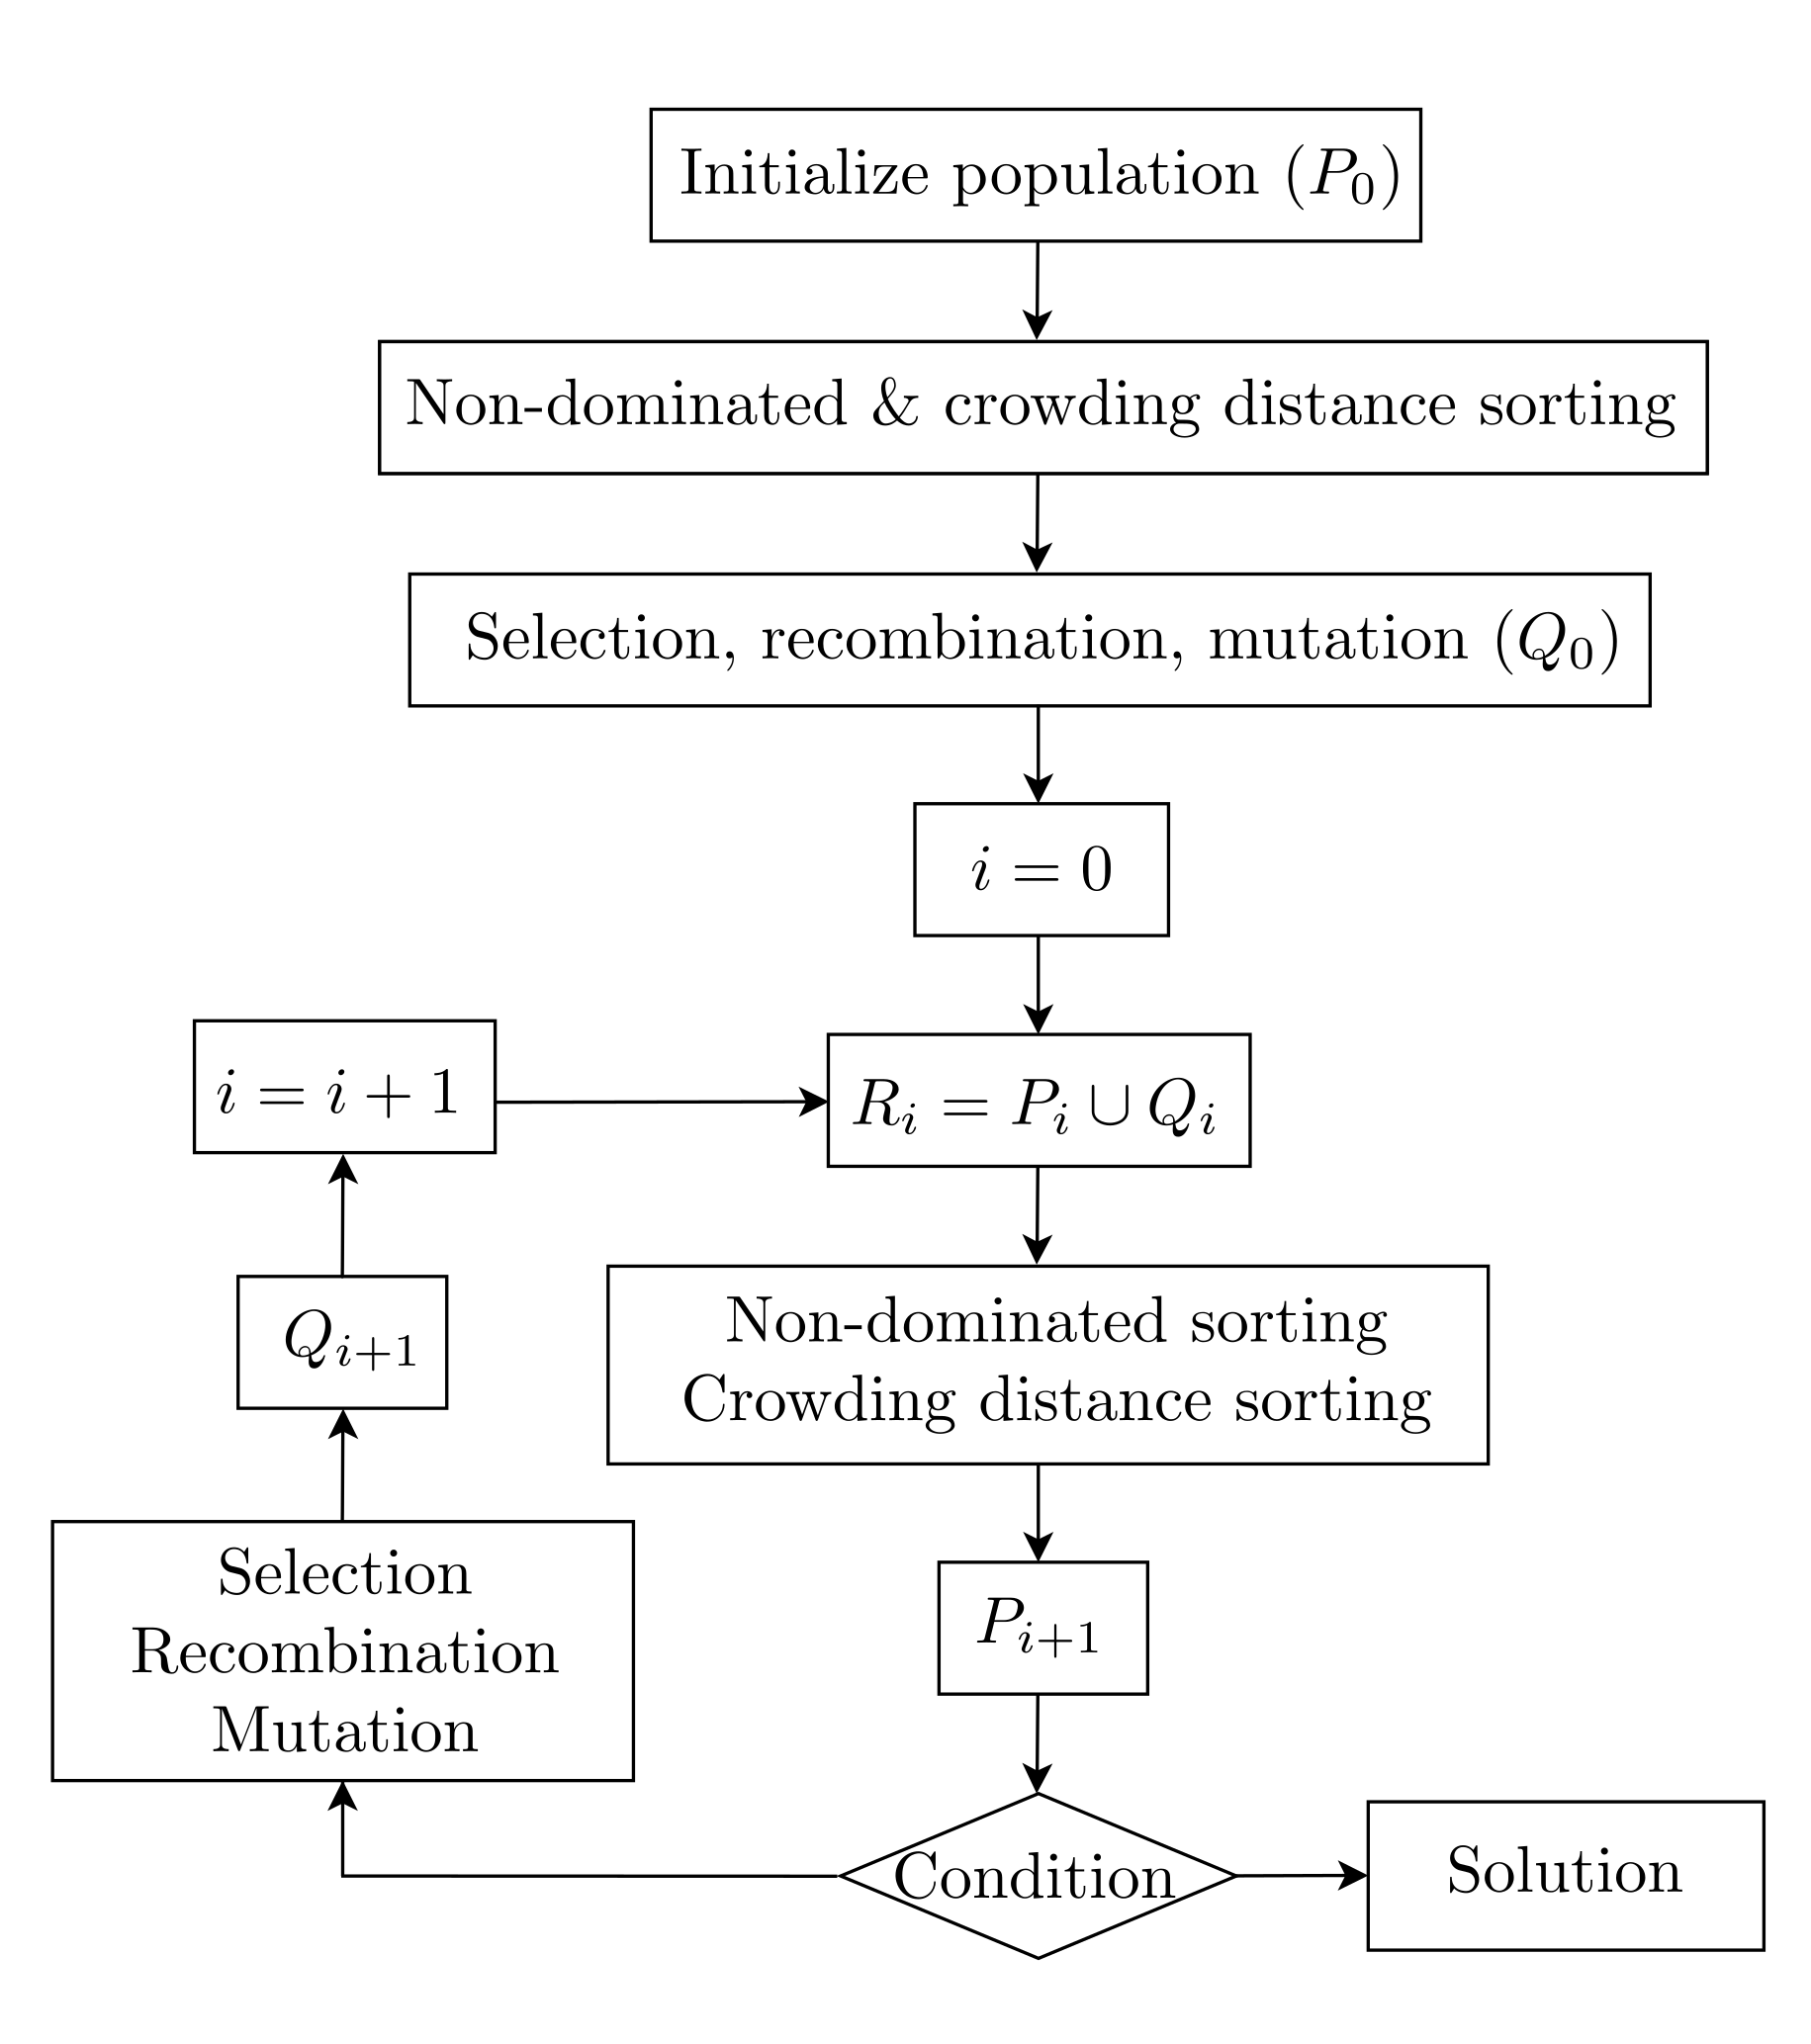
\includegraphics[width=0.6\textwidth]{Figures/2/NSGAflow.png}
        \caption{Chart flow of the NSGA-II algorithm }
        \label{fig:chartFlowNSGAII}
\end{figure}

\newpage

\section{Computer Fluid Dynamics}

Computer fluid dynamics is the analysis of systems involving especially fluid flow (but also heat transfer and chemical reactions) with computer-based simulations. The techniques are very powerful and they may be applied to a wide range of industrial and engineering applications. Although other computer-based simulation, such as stress analysis codes, have a greater capability than CFD codes (due to the incredible complexity of the underlying behavior of fluid flows), the use of CFD is essential in every aspect of the design of a new concept or product. The investment in a CFD code is smaller than the minimum cost of an experimental setup (having even some CFD codes that are completely free). 

Almost all CFD codes work similarly, having very differentiated steps \cite{versteeg1995computational}:
\begin{itemize}
    \item Pre-processor: in this step, the setup of the problem is defined. The computational domain is created with a grid or mesh formed by different cells or control volumes, the set of equations to be solved and the fluid properties are selected in this step and the conditions at the boundary of the domain are established. 
    \item Solver: there are different numerical techniques available for approaching these problems: finite difference (especially the finite volume method), finite element and spectral methods. The numerical algorithm consists on a series of steps: the integration of the governing equation of fluid flow, discretization of the resulting integral equation into an algebraic system of equations and the solution of that algebraic system of equations. 
    \item Post-processor: the output obtained in the solver phase is analyzed and data is extracted in order to draw some conclusions. With the increase of graphic capabilities of engineering workstations, a lot of versatile data visualization tools are used to present data in a more visual way. 
\end{itemize}

The set of governing equations of the flow of a compressible Newtonian fluid that is solved in a computer fluid dynamics code is formed by five partial differential equations (PDEs) with two algebraic equations that supplement the five PDEs. The equations are listed in
\ref{table:cfdEqs}.

\newpage

\begin{table}[htb]
\centering

\caption{Equations of a compressible Newtonian fluid} \label{table:cfdEqs}

\begin{tabular}{
    >{\linespread{1.}\selectfont}m{3.cm}
    @{}
    m{12cm}
    @{}
}

Continuity &
  \tableequation{
    \dfrac{\partial \rho}{\partial t} + \text{div} (\rho \bm{u}) = 0
  \label{eq:continuity}} \\

x-momentum &
  \tableequation{
    \dfrac{\partial (\rho u)}{\partial t} + \text{div} (\rho u \bm{u}) = -\dfrac{\partial p}{\partial x}+\text{div}(\mu \ \text{grad}\ u) +S_{M_x} 
  \label{eq:xmomentum}} \\

y-momentum &
  \tableequation{
    \dfrac{\partial (\rho v)}{\partial t} + \text{div} (\rho v \bm{u}) = -\dfrac{\partial p}{\partial y}+\text{div}(\mu \ \text{grad}\ v) +S_{M_y} 
  \label{eq:ymomentum}} \\

z-momentum &
  \tableequation{
    \dfrac{\partial (\rho w)}{\partial t} + \text{div} (\rho w \bm{u}) = -\dfrac{\partial p}{\partial z}+\text{div}(\mu \ \text{grad}\ w) +S_{M_z} 
  \label{eq:zmomentum}} \\

Energy &
  \tableequation{
    \dfrac{\partial (\rho i)}{\partial t} + \text{div} (\rho i \bm{u}) = -p\ \text{div}\ \bm{u} +\text{div}(k \ \text{grad}\ T) + \bm{\Phi} +S_i
  \label{eq:energy}} \\

\begin{tabular}{@{}c@{}}Equations \\ of state\end{tabular} &
\tableequation{p=p(\rho,T) \text{ and } i=i(\rho, T)
\label{eq:stateEqs}}  \\

 & \tableequation{(\text{for a perfect gas } p=\rho RT \text{ and } i=C_v T ) \nonumber} \\

\end{tabular}

\end{table}

In these equations $\rho$ represents the density of the flow, $\bm{u}$ is the velocity vector with its three components $\bm{u}=(u,v,w)$, $t$ is time, $p$ is the pressure, $\mu$ is the dynamic viscosity, $(x,y,z)$ represent spatial components, $i$ is the internal energy, $k$ is the heat conduction coefficient and $T$ is the temperature. Equations \ref{eq:xmomentum}, \ref{eq:ymomentum} and \ref{eq:zmomentum} have a momentum source $S_M$, while \ref{eq:energy} has an internal energy source term $S_i$ and a dissipation function $\bm{\Phi}$. The set of equations is coupled with the equations of state \ref{eq:stateEqs} which relate temperature and density with pressure and internal energy. 

To solve this system of equations, initial conditions and boundary conditions must be established for the case. Depending on the setup to be solved, this system may be simplified down to a more simpler system with fewer variables and equations (for example, by reducing the 3D analysis in a 2D case or doing a steady state solution where the temporal terms are neglected).
\chapter{Methodology}

\section{Optimization \& Genetic algorithms}

As explained in the previous chapter, there are different ways of approaching a multiobjective optimization problem. Three different ways will be analyzed in order to choose the most appropriate one for the coupling of a search method and computer fluid dynamics: 

\begin{itemize}
    \item Random search: this method is also known as Monte Carlo method. It consists of sampling the search space in a random fashion and hoping to get a good definition of the Pareto front. As said before this kind of methods are not very efficient and in order to achieve high accuracy values, the number of individuals must be big enough. Furthermore, this approach is only efficient in 2 and 3 variable search spaces, given that with more than 3 variables, the search space is too big to cover it with a simple sampling of points.
    \begin{figure}[h!]
        \centering
        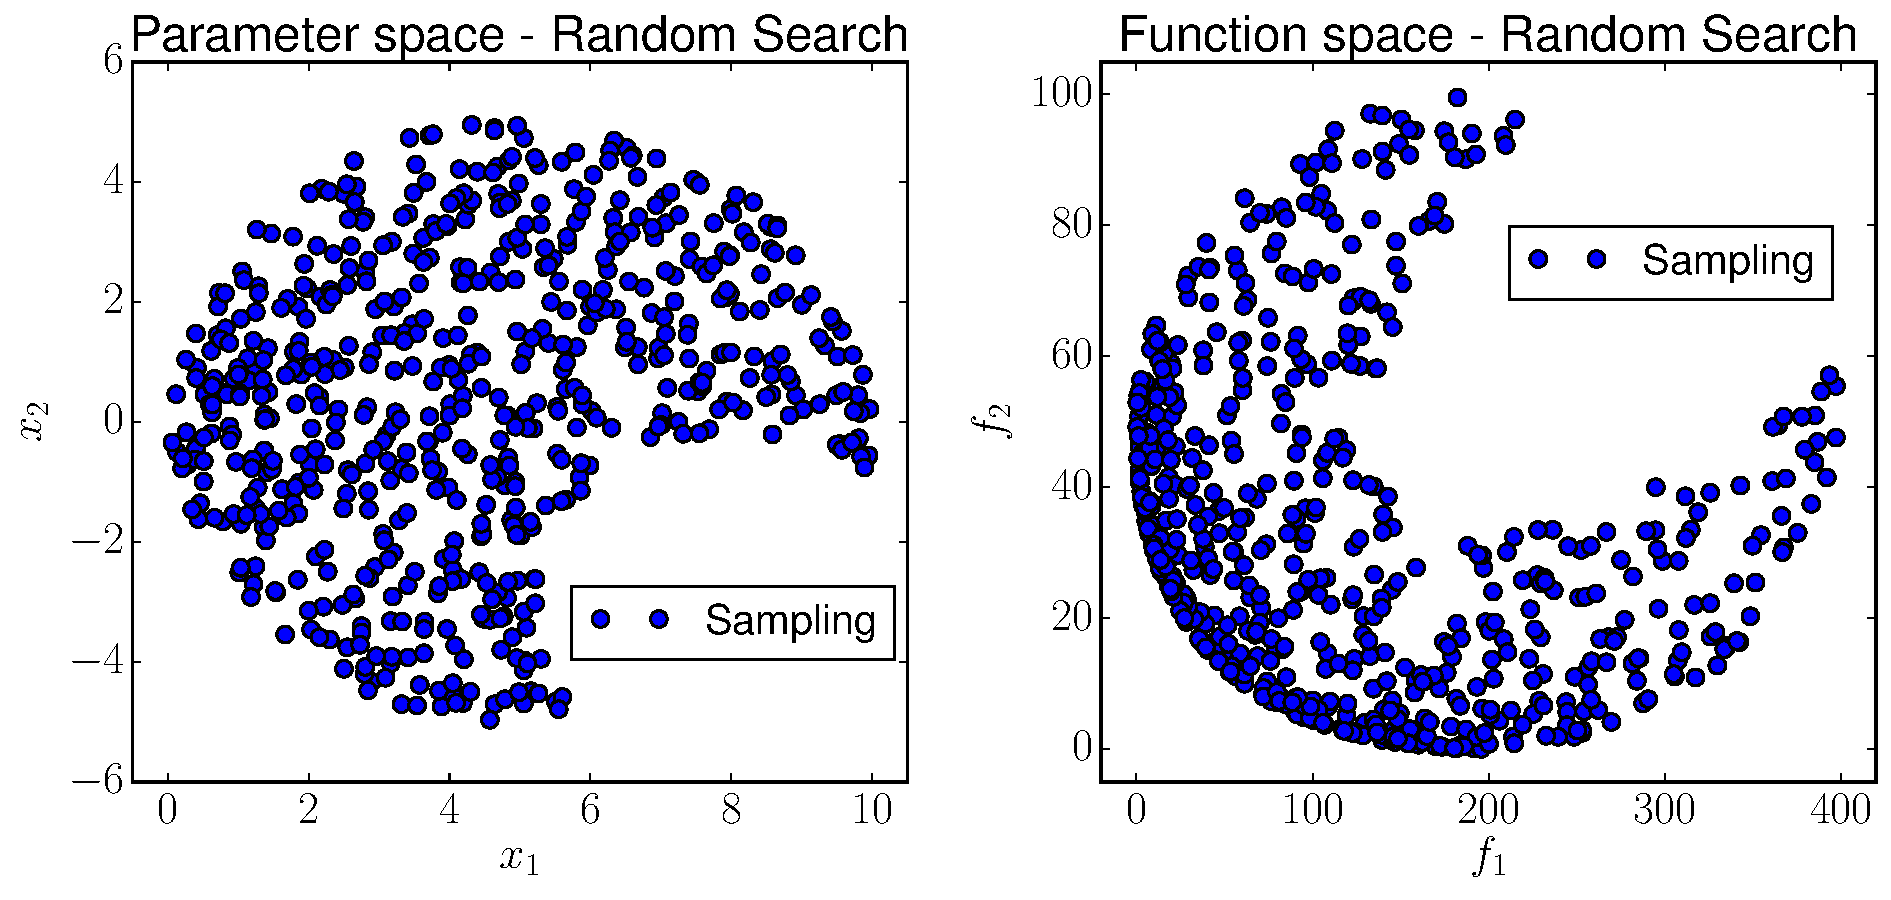
\includegraphics[width=0.85\textwidth]{Figures/3/mode_randomSearch.pdf}
        \caption{Random search method}
        \label{fig:randomSearch}
    \end{figure}
    \item General genetic algorithm: a general GA was coded up in Python. This GA may be used for a great variety of tasks and it is not designed for multiobjective optimization problems. Fitness is assigned with the distance to the Pareto front of each one of the individuals. The selection method chosen is the roulette method, with linear crossover and normal distribution mutation. The results obtained with this method show the Pareto front and how the individuals converge towards it along generations.     \begin{figure}[h!]
        \centering
        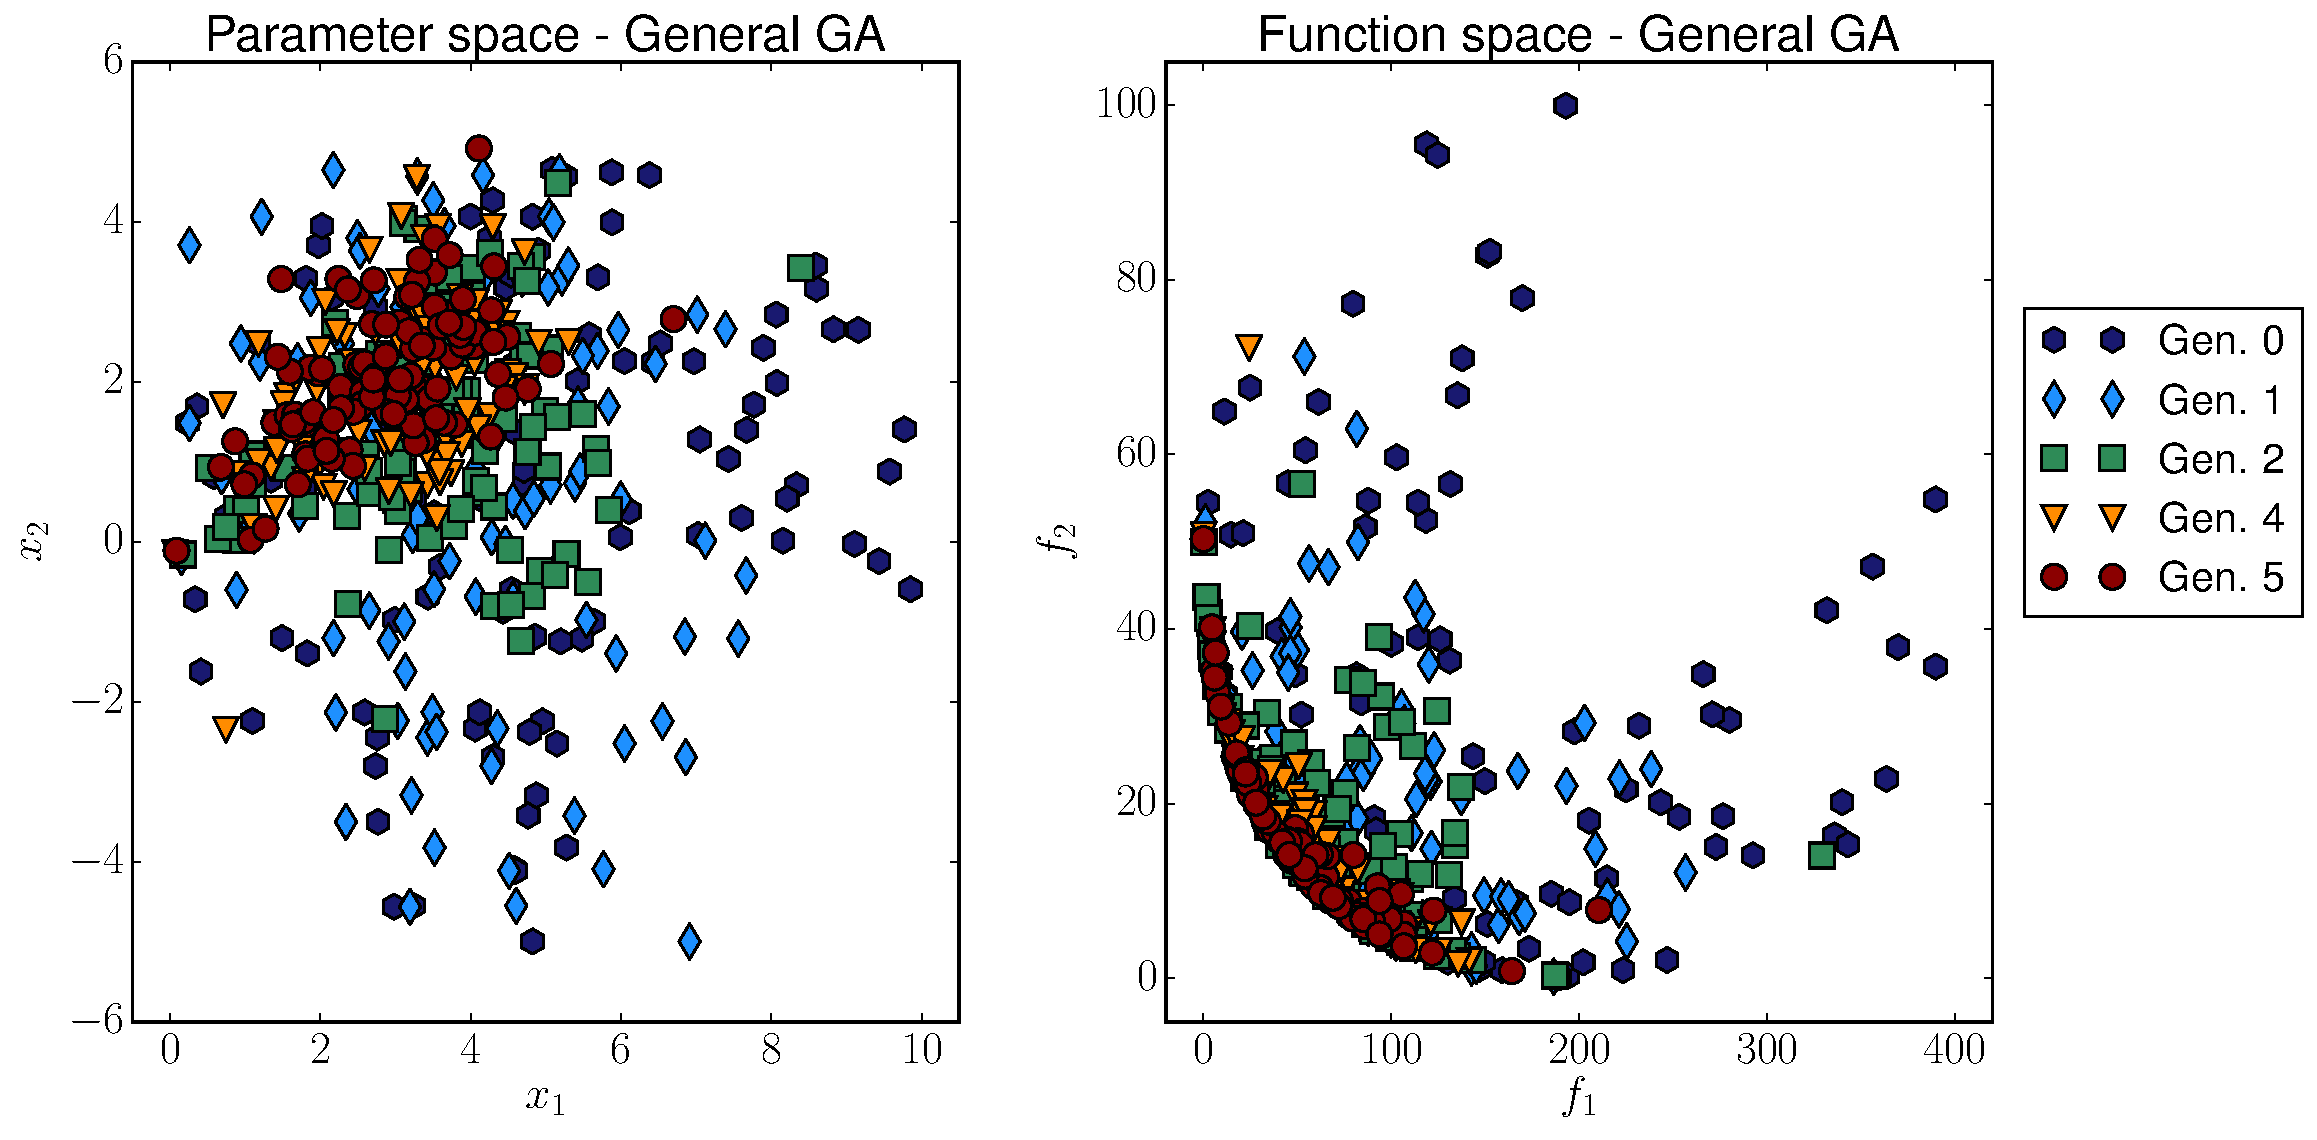
\includegraphics[width=0.8\textwidth]{Figures/3/mode_generalGAE.pdf}
        \caption{General genetic algorithm}
        \label{fig:plainGeneticAlgorithm}
    \end{figure}
    \item NSGA-II: the non-dominated sorting genetic algorithm is described in \cite{deb2002fast} and it is specially designed for multiobjective optimization problems. It is expected to have a greater convergence and more possibilities of capturing the whole Pareto front than the previously mentioned GA:
    \begin{figure}[h!]
        \centering
        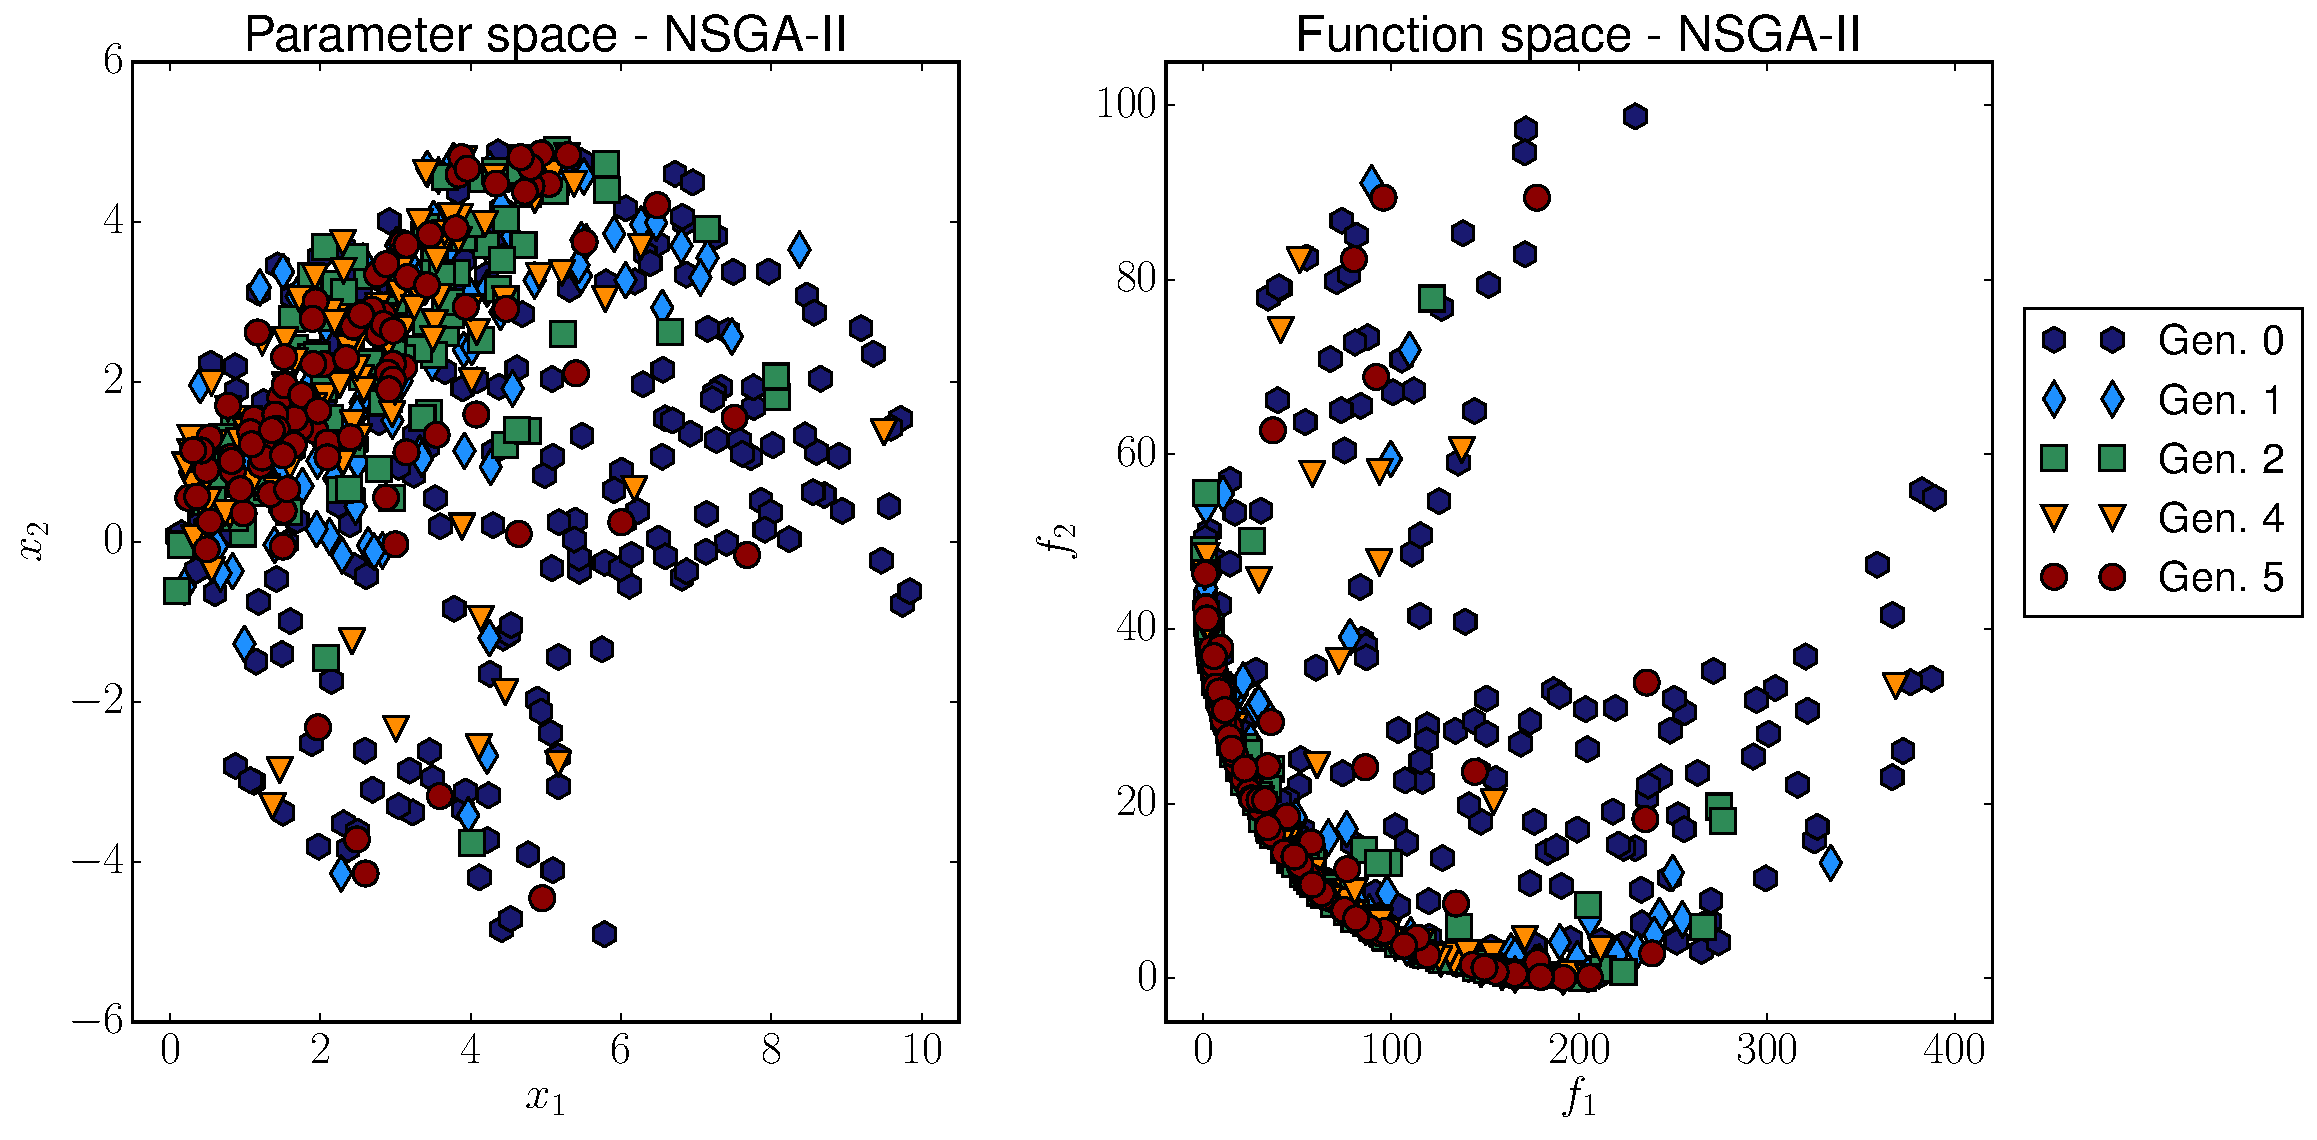
\includegraphics[width=0.8\textwidth]{Figures/3/mode_NSGA.pdf}
        \caption{Non-dominated sorted genetic algorithm II}
        \label{fig:NSGA-IIworkingMode}
    \end{figure}
\end{itemize}

\newpage

\subsection{Comparison of the performance of different methods}

The main question now is which one of these three methods will perform better, i.e., which one captures a more spread and precise Pareto front. The three methods searched the solution for different multiobjective optimization test functions, computing a histogram to show which is the probability of having an individual in certain area of the search and fitness spaces. Sixteen runs were performed, using the values shown in Table \ref{table:RSvsGAEvsNSGA}. It may be seen that the individuals in the random search are the same as the number of evaluations. Also for the general GA the number of individuals times the number of generations yields the number of evaluations. However, for the NSGA-II case, numbers don't add up at first glance because the first population of the NSGA-II is initialized with a population twice the size ($2N$) of the rest of the populations ($N$).

\begin{table}[H]
\centering
\renewcommand{\arraystretch}{1.1}
\caption{Different configurations for the different possibilities}
\label{table:RSvsGAEvsNSGA}
\begin{tabular}{|c|c|c|c|c|c|}
\hline
{\begin{tabular}[c]{@{}c@{}}RANDOM\\ SEARCH\end{tabular}} & \multicolumn{2}{c|}{{\begin{tabular}[c]{@{}c@{}}GENERAL\\ GA\end{tabular}}} & \multicolumn{2}{c|}{{NSGA-II}} & \multirow{2}{*}{{\begin{tabular}[c]{@{}c@{}}NUMBER OF \\ EVALUATIONS\end{tabular}}} \\ \cline{1-5}
{Indiv.} & {Indiv.} & {Gener.} & {Indiv.} & {Gener.} &  \\ \hline
80 & 10 & 8 & 10 & 7 & 80 \\ \hline
90 & 10 & 9 & 10 & 8 & 90 \\ \hline
100 & 10 & 10 & 10 & 9 & 100 \\ \hline
110 & 10 & 11 & 10 & 10 & 110 \\ \hline
200 & 25 & 8 & 25 & 7 & 200 \\ \hline
225 & 25 & 9 & 25 & 8 & 225 \\ \hline
250 & 25 & 10 & 25 & 9 & 250 \\ \hline
275 & 25 & 11 & 25 & 10 & 275 \\ \hline
450 & 50 & 9 & 50 & 8 & 450 \\ \hline
500 & 50 & 10 & 50 & 9 & 500 \\ \hline
550 & 50 & 11 & 50 & 10 & 550 \\ \hline
600 & 50 & 12 & 50 & 11 & 600 \\ \hline
900 & 100 & 9 & 100 & 8 & 900 \\ \hline
1000 & 100 & 10 & 100 & 9 & 1000 \\ \hline
1100 & 100 & 11 & 100 & 10 & 1100 \\ \hline
1200 & 100 & 12 & 100 & 11 & 1200 \\ \hline
\end{tabular}
\end{table}

Genetic algorithms are usually run for 25000 iterations, with populations of 250 individuals. However, here the number of function evaluations is way lower because when applied to CFD, several minutes will take the evaluation of each individual (whereas for a function optimization, a whole population evaluation may last seconds).

\newpage

The test functions used were:
\begin{itemize}
\item \textbf{Bihn \& Korn test function:} this function was already described before (\ref{eq:BihnKorn}) but it is added here again for clarification. This is a function-constrained search optimization, with two objectives and two variables:
    \begin{equation}
        \begin{array}{cl}
            \textrm{minimize} & 
            \left\{ \begin{array}{l}
                f_1(x_1,x_2) = 4x_1^2 + 4x_2^2\\
                f_2(x_1,x_2) = (x_1-5)^2+(x_2-5)^2
            \end{array} \right. \\
            & \\
            \textrm{subject to} &  
            \left\{ \begin{array}{l}
                (x_1-5)^2+x_2^2-25 \leq 0\\
                -(x_1-8)^2-(x_2+3)^2 + 7.7 \leq 0
            \end{array} \right. \\
            & \\
            \textrm{bounded by} & -15 \leq x_i \leq 30, \ \ \forall i = 1,2
        \end{array}
        \tag{\ref{eq:BihnKorn} revisited}
    \end{equation}

\item \textbf{Poloni's test function:} two objectives and two variables test function \cite{poloni1995hybrid}:
    \begin{equation}
\begin{array}{cl}
            \textrm{minimize} & 
            \left\{ \begin{array}{l}
                f_1(x_1,x_2) = 1+\left[A_1-B_1(x_1,x_2)\right]^2+\left[A_2-B_2(x_1,x_2)\right]^2\\
                f_2(x_1,x_2) = (x_1+3)^2+(x_2+1)^2
            \end{array} \right. \\
            & \\
            \textrm{where} & 
            \left\{ \begin{array}{l}
                A_1 = 0.5\sin(1)-2\cos(1)+\sin(2)-1.5\cos(2) \\
                A_2 = 1.5\sin(1)-\cos(1)+2\sin(2)-0.5\cos(2) \\
                B_1(x_1,x_2) = 0.5\sin(x_1)-2\cos(x_1)+\sin(x_2)-1.5\cos(x_2) \\
                B_2(x_1,x_2) = 1.5\sin(x_1)-\cos(x_1)+2\sin(2)-0.5\cos(x_2)
            \end{array} \right. \\
            & \\
            \textrm{in} & -\pi \leq x_i \leq \pi, \ \ \forall i = 1,2
        \end{array}
        \label{eq:poloni}
    \end{equation}

\item \textbf{Zitzler-Deb-Thiele's test functions:} ZDT are a classical set of test functions designed for genetic algorithms to test its performance. They are designed for 30 variables and bi-objective optimization, but in this case, the ZDT2 function was adapted to just two variables in the search space \cite{zitzler2000comparison}:
    \begin{equation}
\begin{array}{cl}
            \textrm{minimize} & 
            \left\{
             \arraycolsep=1.0pt\def\arraystretch{2.0} \begin{array}{l}
            f_1(x_1,x_2) = x_1\\
            f_2(x_1,x_2) = g(x_1,x_2) \cdot h(f_1(x_1,x_2),g(x_1,x_2))\\
            g(x_1,x_2) = 1+\dfrac{9x_2}{29} \\
            h(x_1,x_2) = 1 - \sqrt{\dfrac{x_1}{x_2}}
            \end{array} \right. \\
            & \\
           \textrm{bounded by} & 0 \leq x_i \leq 1, \ \ \forall i = 1,2
        \end{array}
        \label{eq:ZDT2}
    \end{equation}
\end{itemize}

\newpage

    \begin{figure}[H]
        \centering
        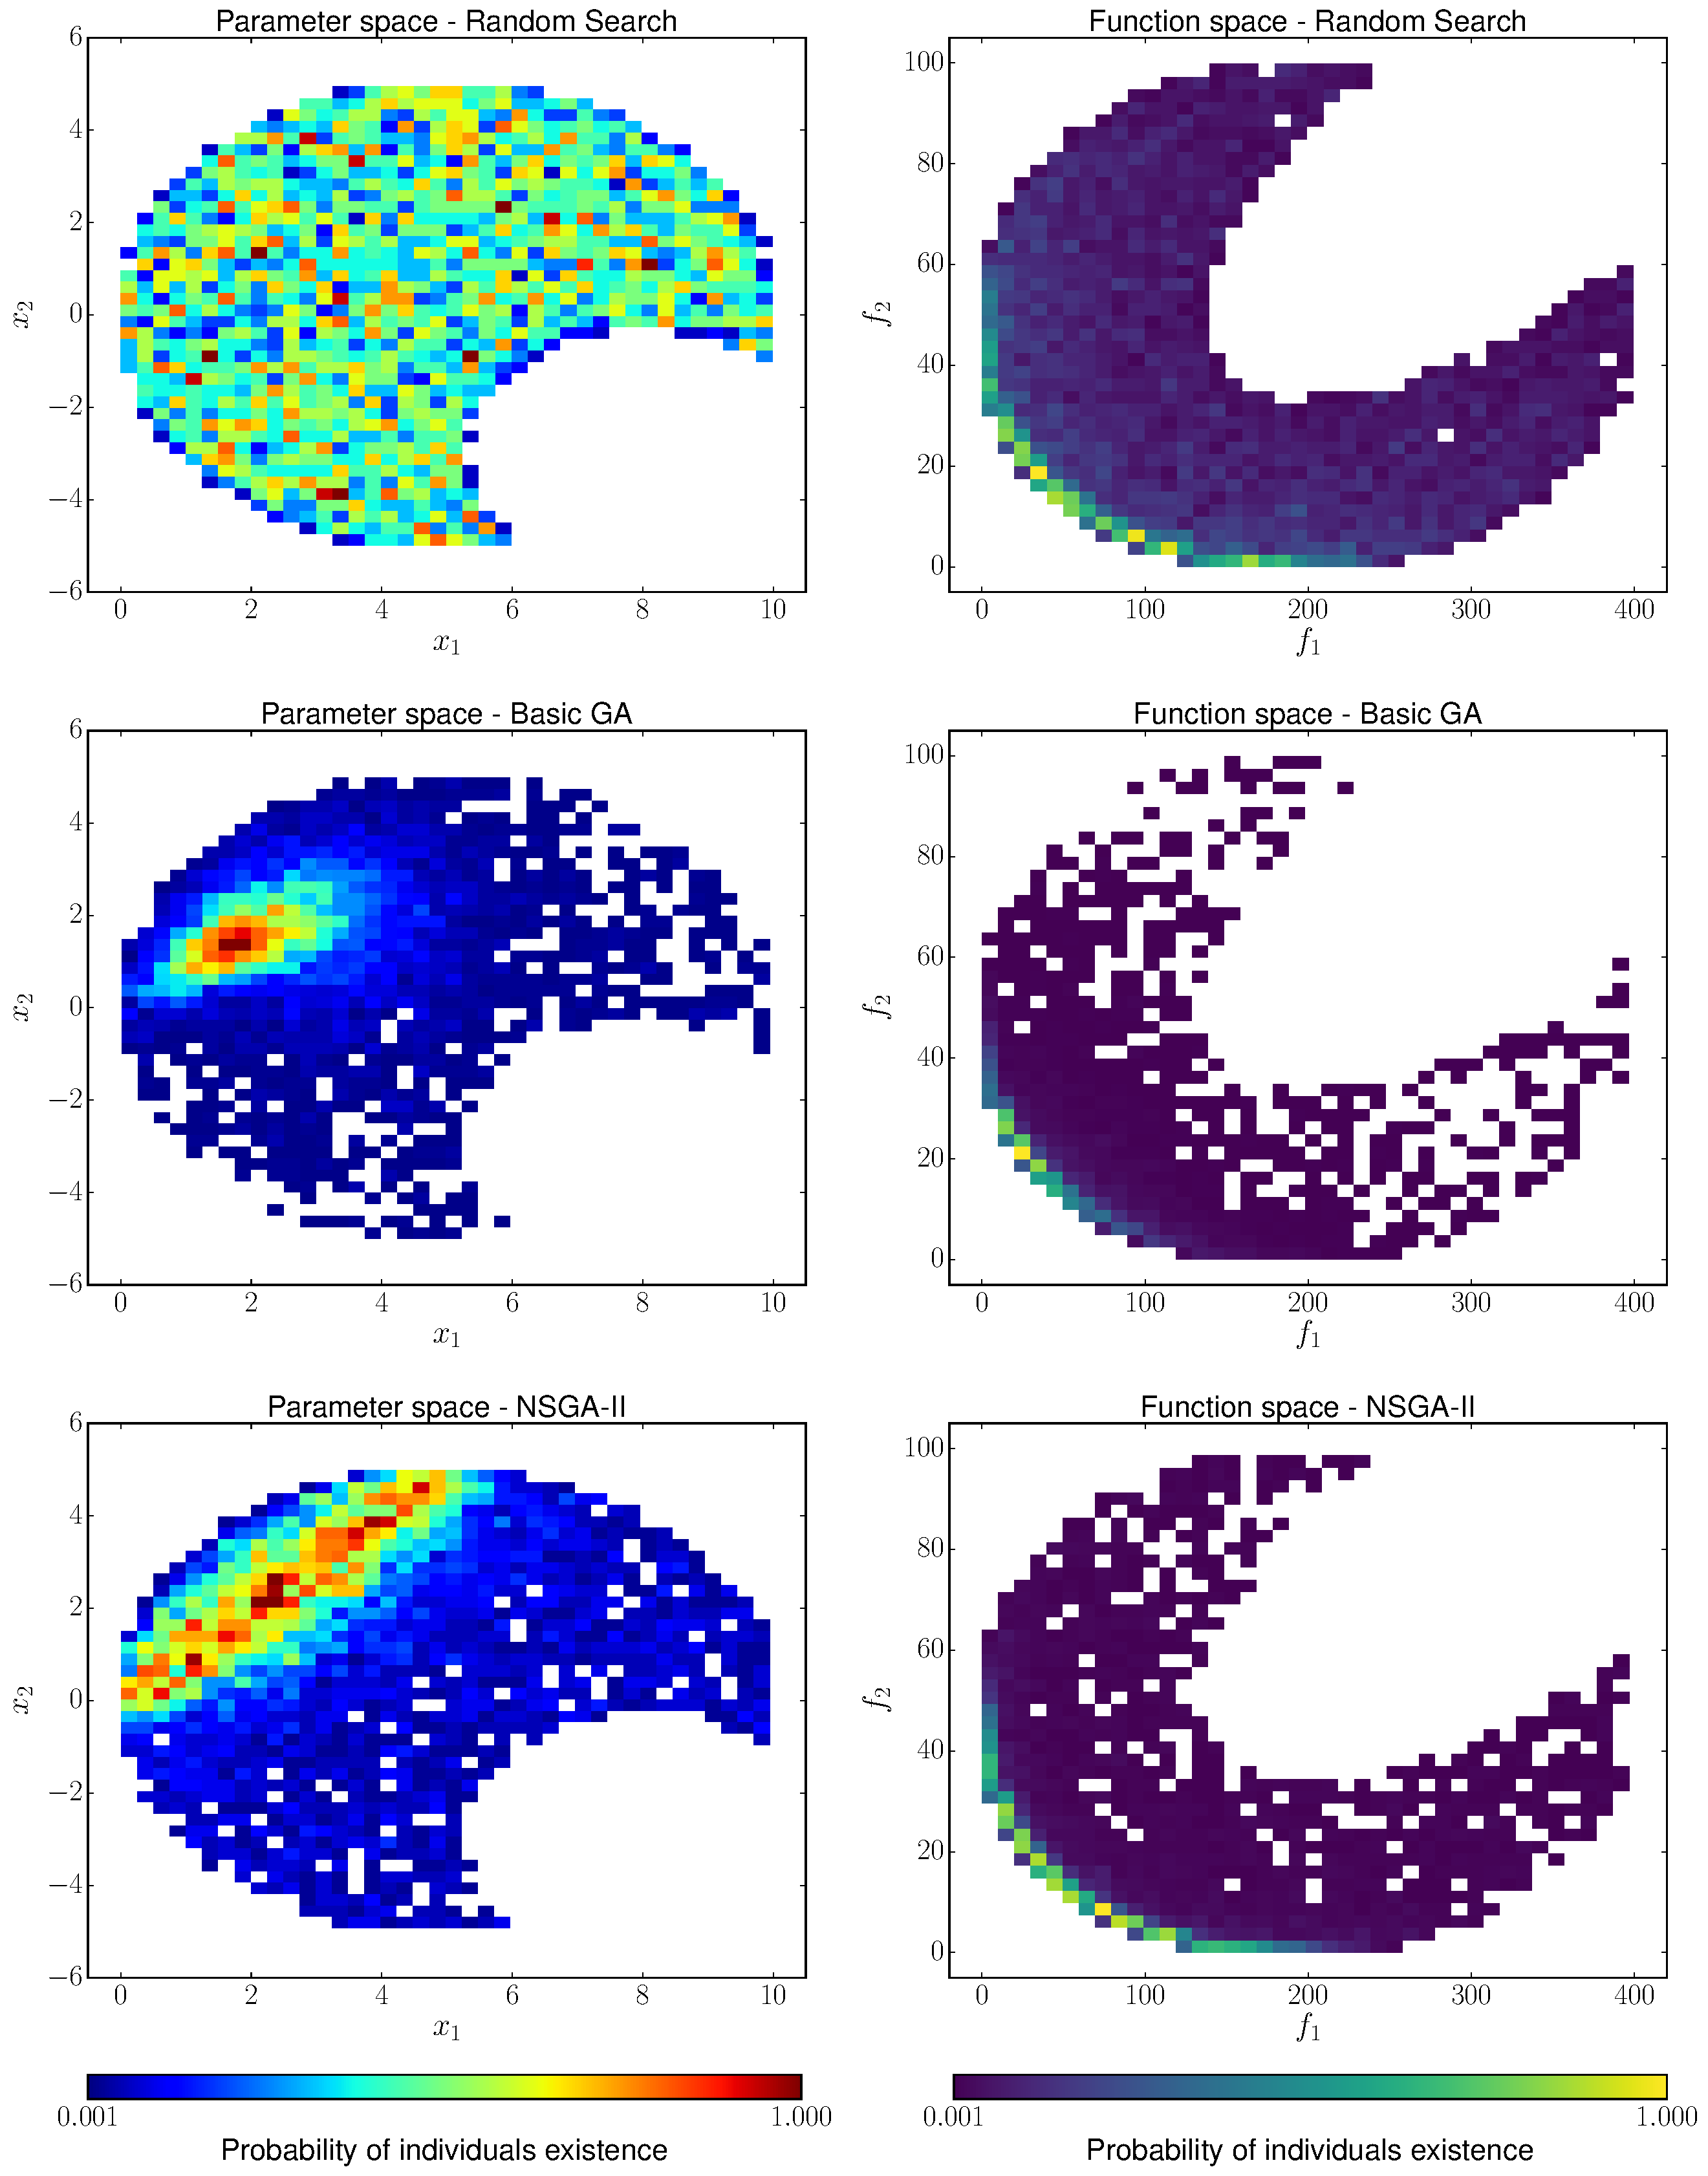
\includegraphics[height=0.96\textheight, width=\textwidth]{Figures/3/hist_BK.pdf}
        \caption{Method comparison for the Bihn \& Korn function}
        \label{fig:histogramBK}
    \end{figure}
    
\newpage

    \begin{figure}[H]
        \centering
        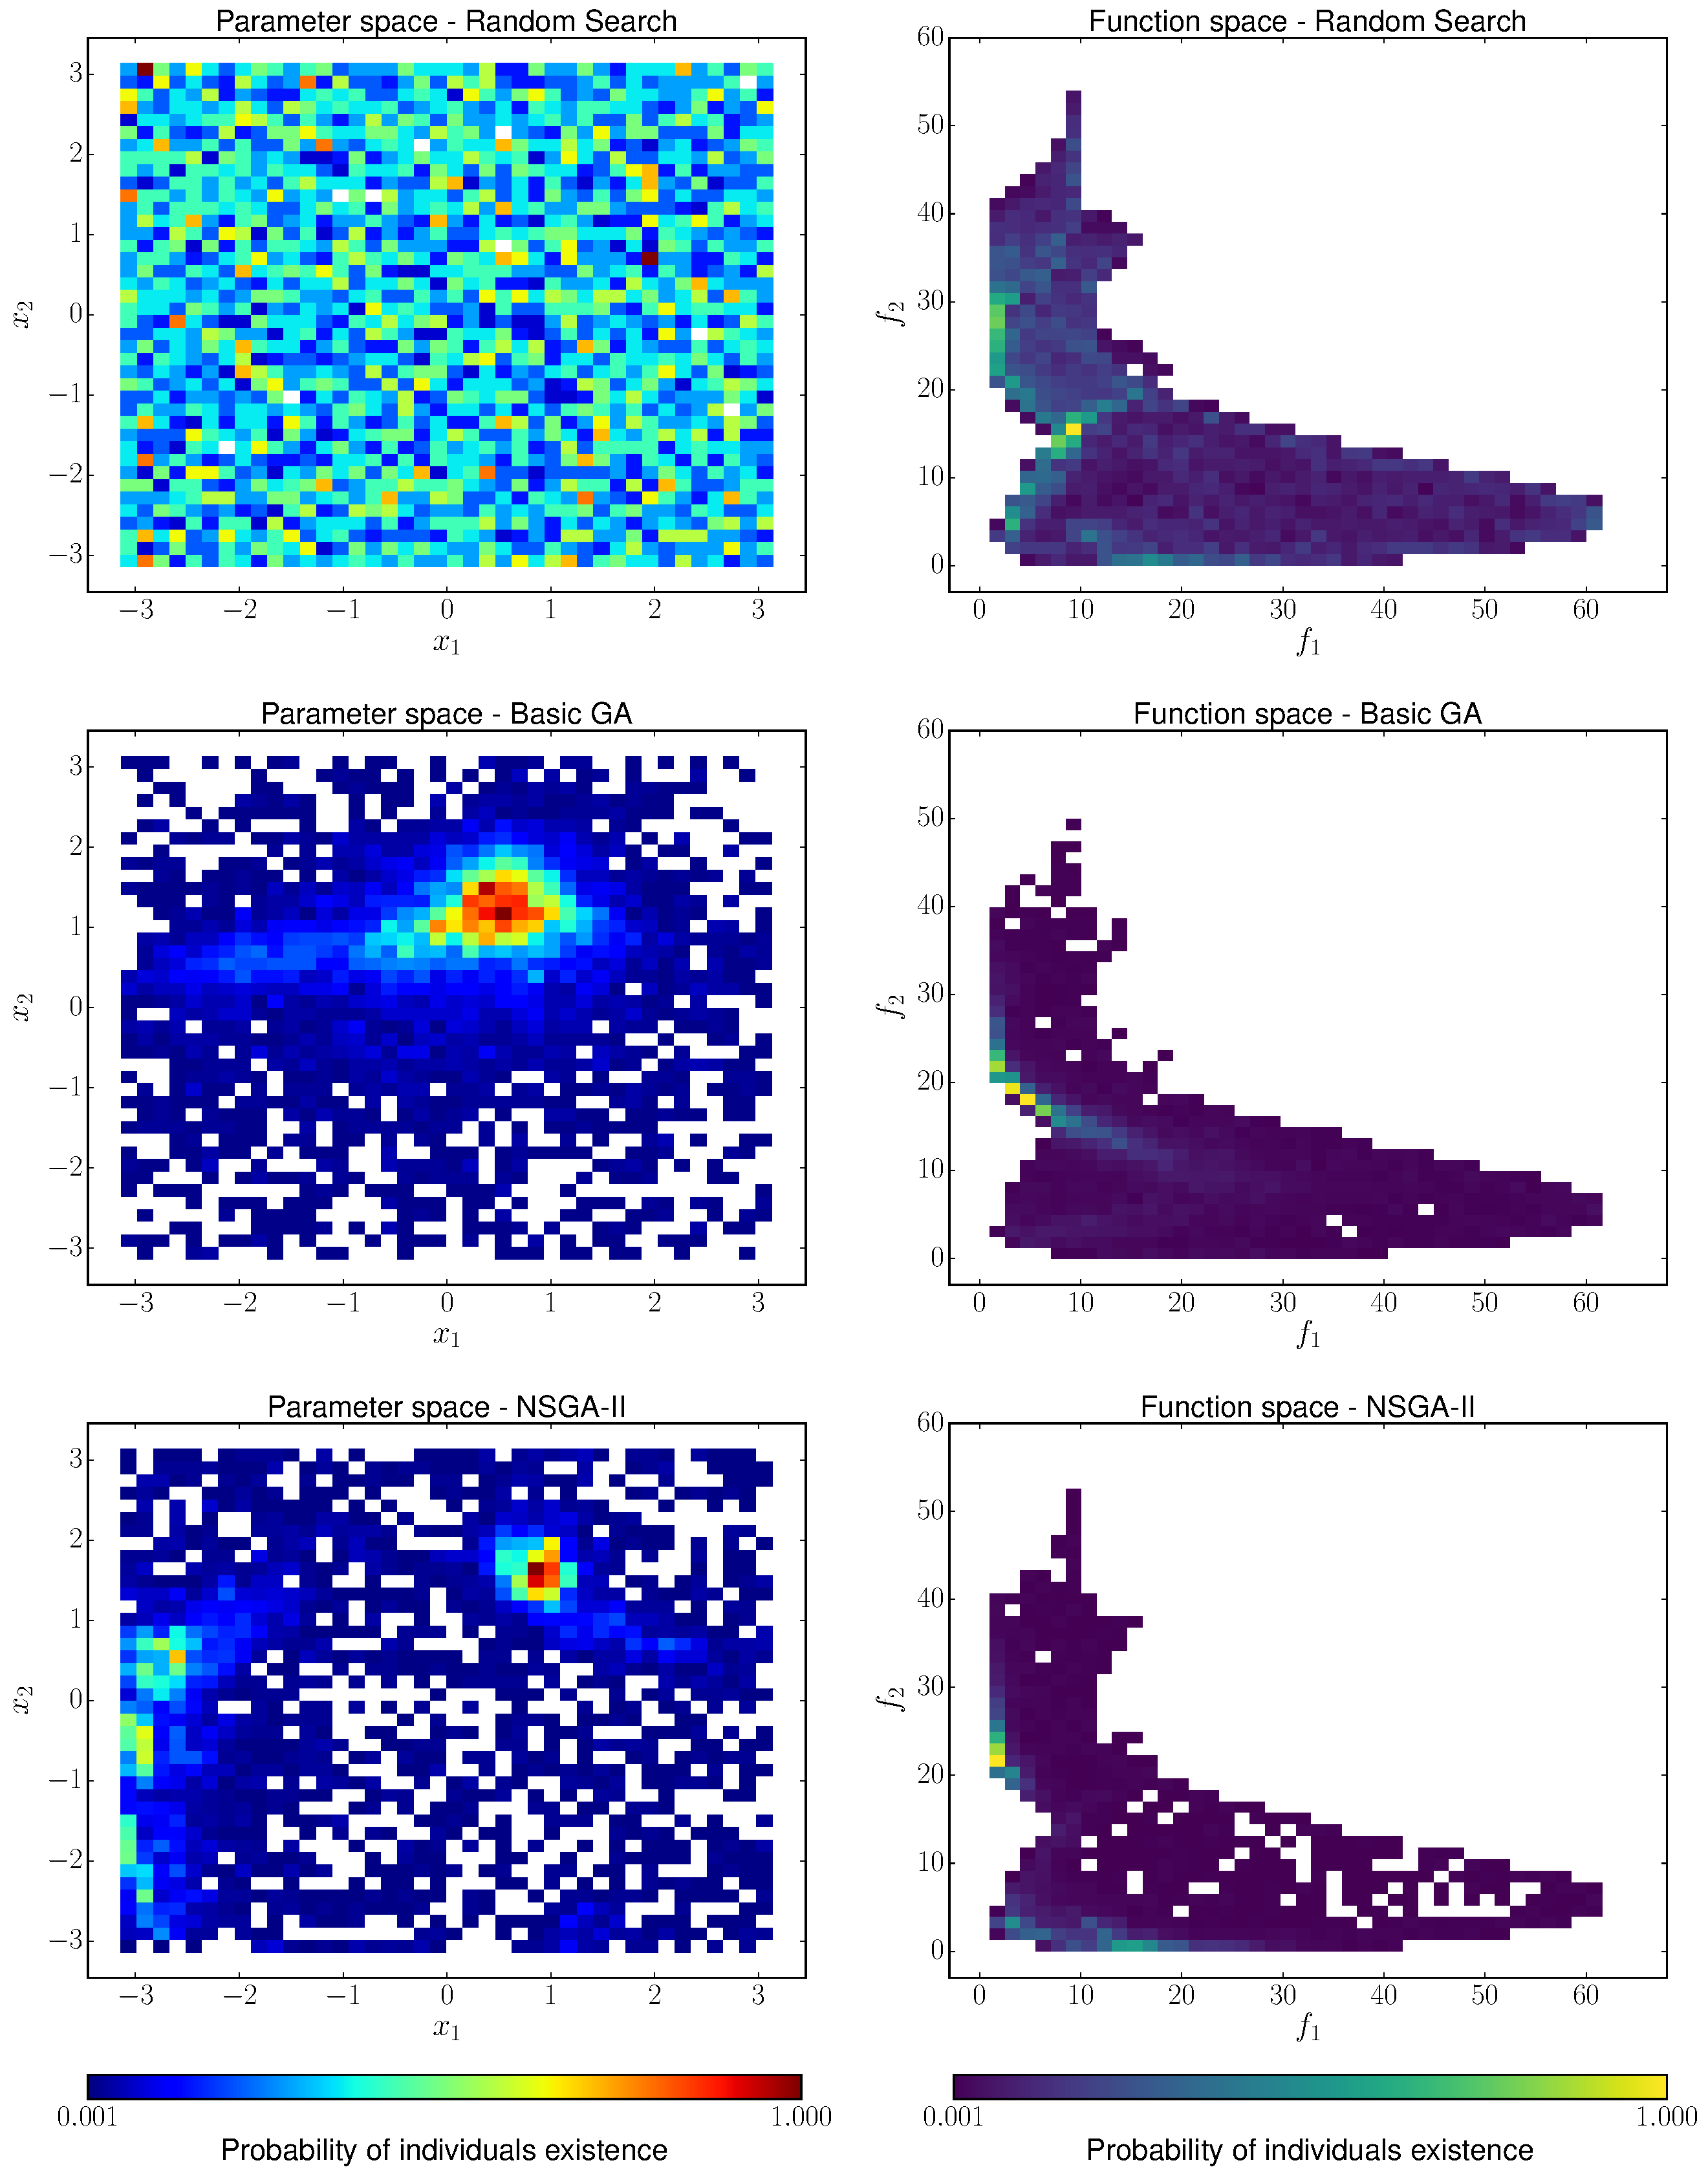
\includegraphics[height=0.96\textheight, width=\textwidth]{Figures/3/hist_POL.pdf}
        \caption{Method comparison for the Poloni's function}
        \label{fig:histogramPOL}
    \end{figure}
    
\newpage

    \begin{figure}[H]
        \centering
        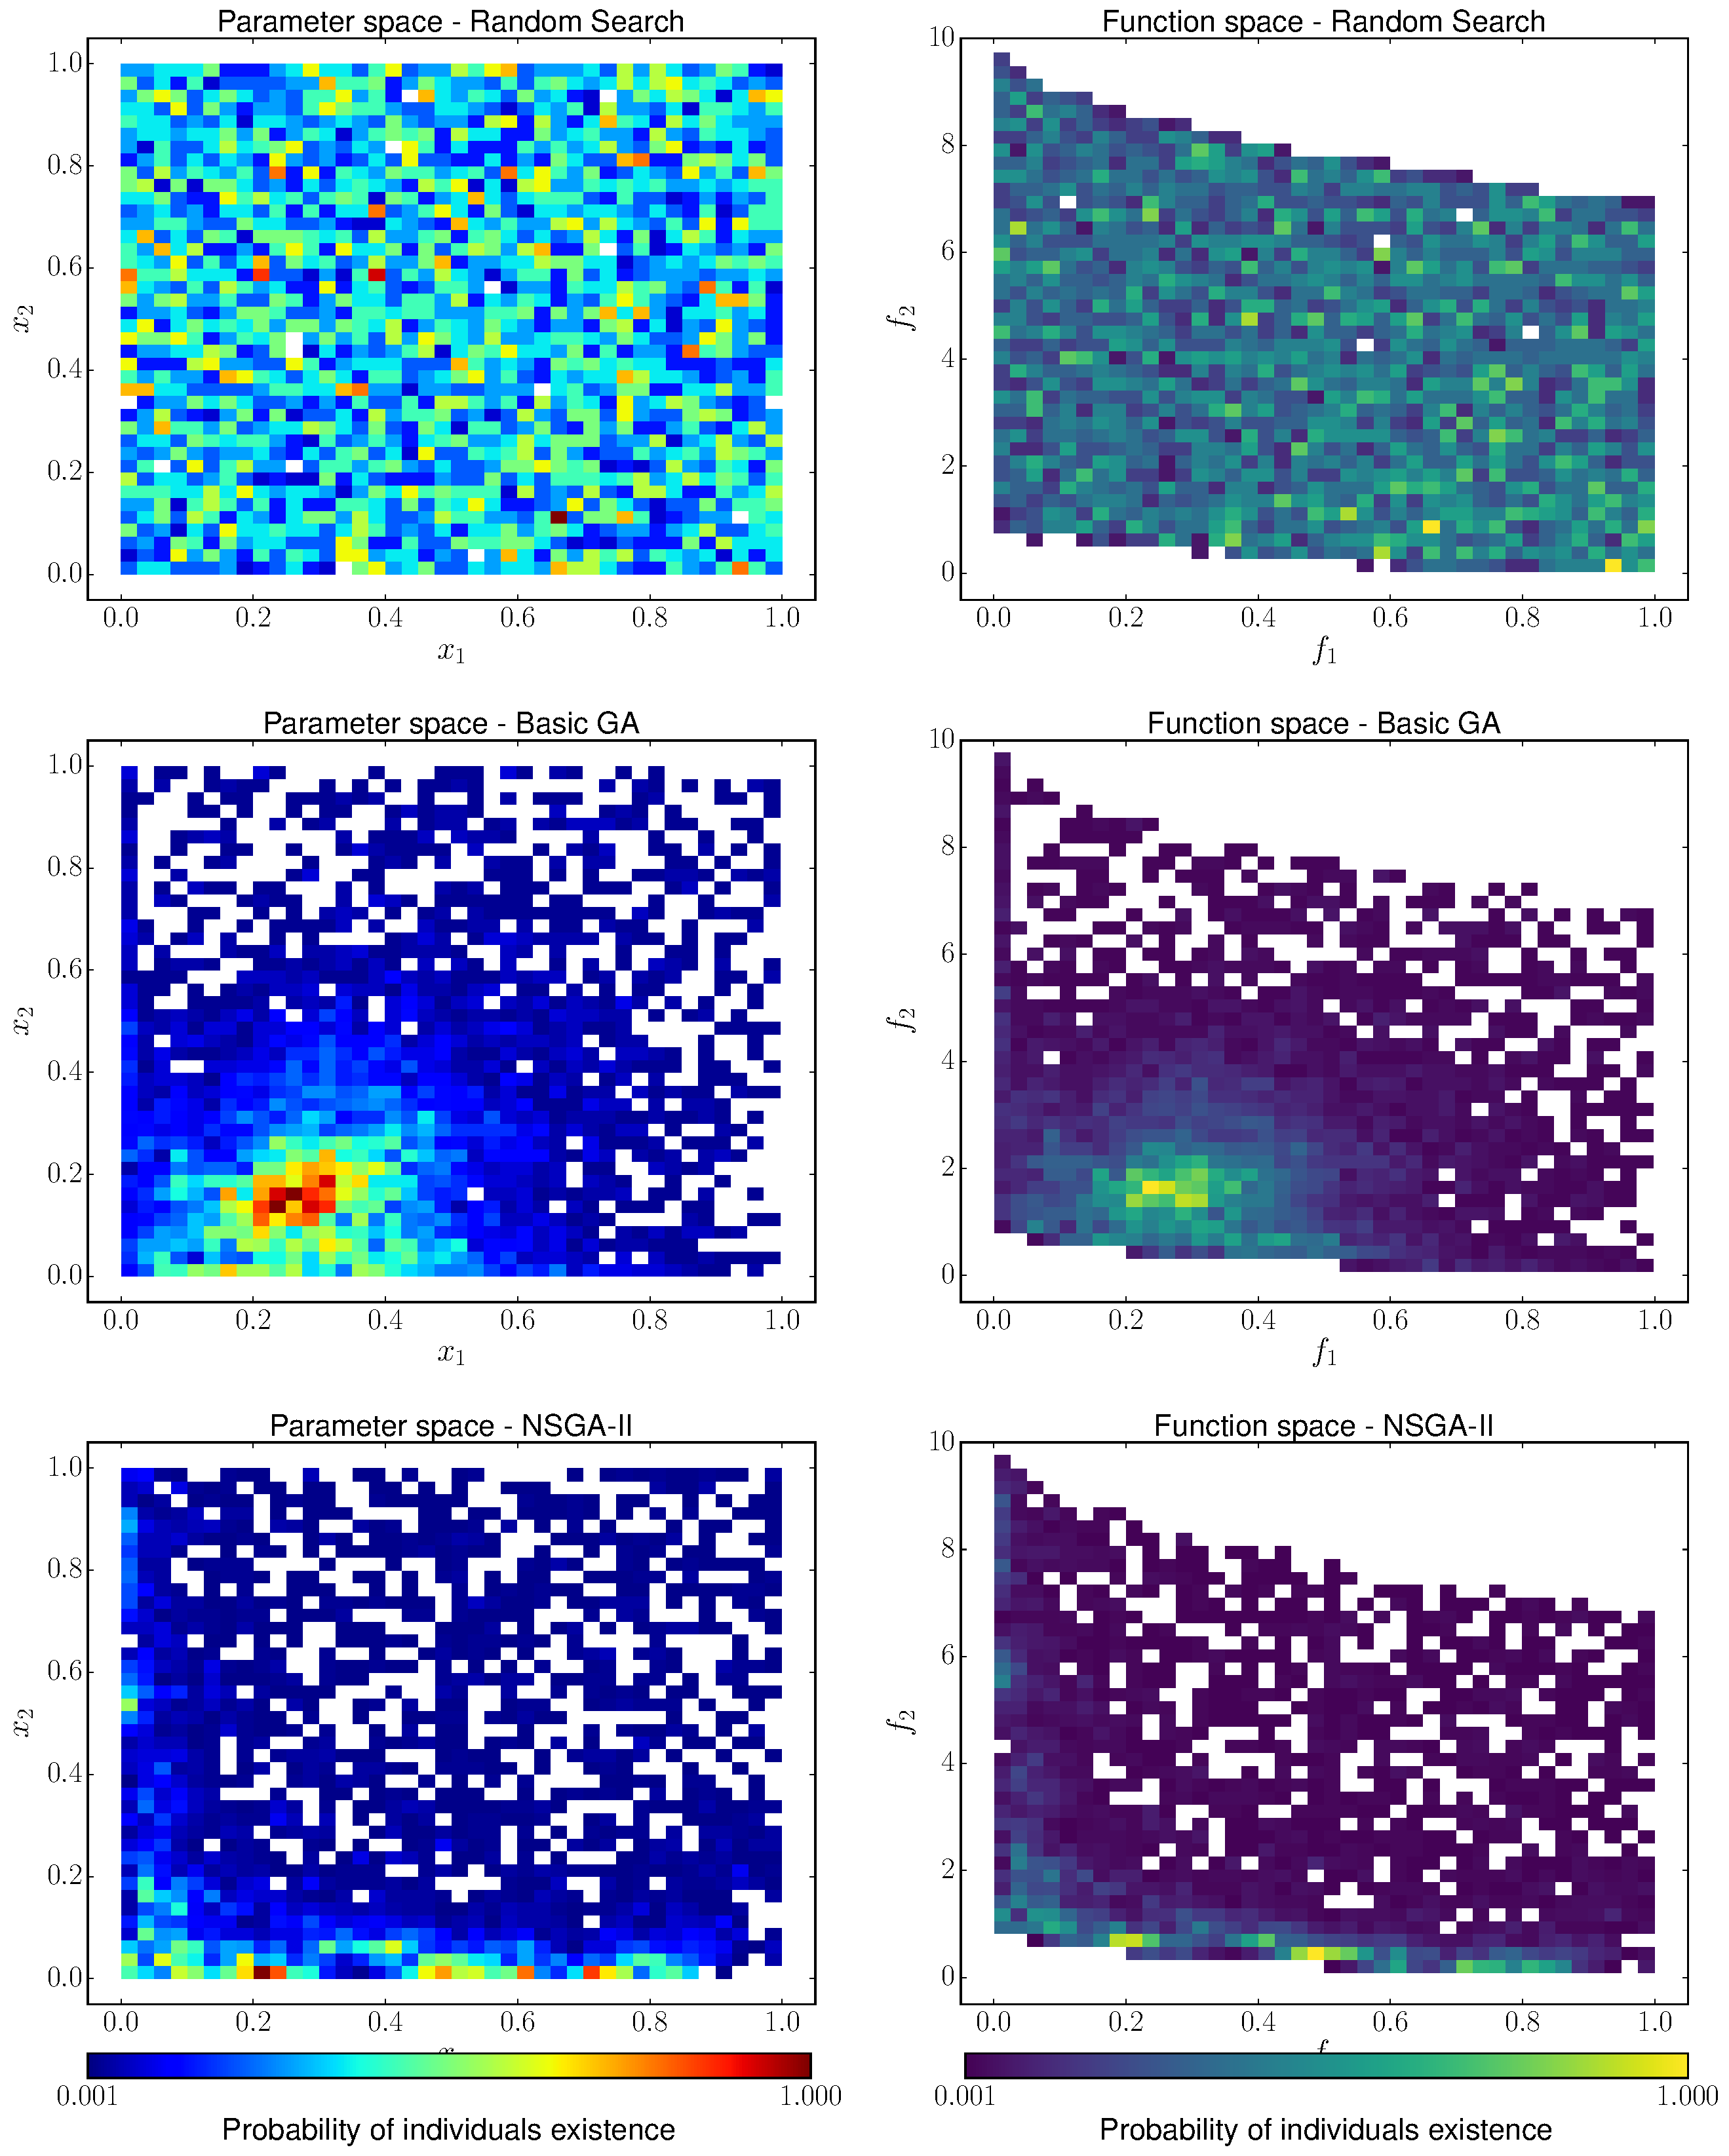
\includegraphics[height=0.96\textheight, width=\textwidth]{Figures/3/hist_ZDT2.pdf}
        \caption{Method comparison for the ZDT2 function}
        \label{fig:histogramZDT2}
    \end{figure}
    
\newpage

It can be seen that for the three functions, the random search cover the whole parameter space uniformly. However, this does not mean that the function space is better analyzed in the surroundings of the Pareto front (see Figure \ref{fig:histogramZDT2}). Thus the random search is not valid even for a two variable case because it does not converge nor evolve towards a solution. The basic GA and the NSGA-II points converge to certain areas, although the basic GA does not cover the whole Pareto front as it should (see Figure \ref{fig:histogramPOL}) or does not capture it at all (see Figure \ref{fig:histogramZDT2}). Thus the only method that is really valid for searching in complex parameter spaces and converge to a true Pareto front is the NSGA-II (see Figures \ref{fig:histogramBK}, \ref{fig:histogramPOL} and \ref{fig:histogramZDT2}). Although this comparison may be seen biased for the different algorithms, the optimization in CFD is usually performed with Monte Carlo methods which are a random search that may not be the most effective methods. 

\subsection{Number of evaluations versus number of generations}

Given that NSGA-II is the algorithm chosen for solving multiobjective optimization problems, a deep knowledge of how the dynamics of the system really work is essential to achieve an accurate solution. The NSGA-II depends only on two variables, which are the number of individuals per generation and the limit in the number of generations. The same number of function evaluations (translated in the future to CFD simulations) may be distributed in different combinations of individuals and generations. In order to prove if it is better to have more individuals or generations (for the same number of function evaluations) two measures proposed by \cite{deb2002fast} are used:
\begin{itemize}
    \item Diversity metric ($\Delta$): it measures the extent of spread achieved in the solutions by taking the distance between each one of the points that form the Pareto-optimal front. The best value will be zero, having that all individuals are at the same distance one to each other. This metric is only valid for bi-objective optimization, but a Voronoi triangularization may be used for Pareto front in higher dimensions: 
    \begin{equation}
        \displaystyle \Delta = \dfrac{d_f+d_l+\sum^{N-1}_{i=1}|d_i-\bar{d}|}{d_f+d_l+(N-1)\bar{d}}
    \end{equation}
\item Convergence metric ($\Upsilon$): this metric may only be used in cases where the Pareto front may be known, because it is defined as the minimum distance to the true Pareto front ($\mathcal{PF}_0$):
\begin{equation}
    \Upsilon =  \text{min} (\text{dist}({PF_{GA}}_i,\mathcal{PF}_0)) 
\end{equation}
\end{itemize}


\newpage

The three test functions described before (\ref{eq:BihnKorn}, \ref{eq:poloni} and \ref{eq:ZDT2}) are used again as a way of knowing how the algorithm really behaves. They were tested with all the cases shown in the Table \ref{table:nubmerofgen}, running each one of the possible configurations 20 times in order to capture the dynamics of the configurations.

\begin{table}[H]
\centering
\renewcommand{\arraystretch}{1.6}
\caption{Generations and individuals combinations tested for performance}
\label{table:nubmerofgen}
\begin{tabular}{c|c|c|c|c|c}
\cline{2-6}
 & \multicolumn{5}{c|}{\textbf{INDIVIDUALS PER GENERATION}} \\ \hline
\multicolumn{1}{|c|}{\textbf{\begin{tabular}[c]{@{}c@{}}TOTAL FUNCTION\\ EVALUATIONS\end{tabular}}} & \textbf{8} & \textbf{16} & \textbf{32} & \textbf{64} & \multicolumn{1}{c|}{\textbf{128}} \\ \hline
\multicolumn{1}{|c|}{\textbf{640}} & 79 & 39 & 19 & 9 & \multicolumn{1}{c|}{4} \\ \hline
\multicolumn{1}{|c|}{\textbf{512}} & 63 & 31 & 15 & 7 & \multicolumn{1}{c|}{3} \\ \hline
\multicolumn{1}{|c|}{\textbf{384}} & 47 & 23 & 1 & 5 & \multicolumn{1}{c|}{2} \\ \hline
\multicolumn{1}{|c|}{\textbf{256}} & 31 & 15 & 7 & 3 & \multicolumn{1}{c|}{\textit{(trivial)}} \\ \hline
\multicolumn{1}{|c|}{\textbf{128}} & 15 & 7 & 3 & \textit{(trivial)} &  \\ \cline{1-5}
\end{tabular}
\end{table}

As said before, it must be noted that the first generation of the NSGA-II has twice the size of the rest of populations. This also created some \textit{trivial} cases, because if the number of individuals is $N$ and the total function evaluations are fixed to be $2N$, the first population will cover all the possible function evaluations (so it will be a random search and not an evolutionary computation algorithm). 

The values shown in the figures are the mean and standard deviation of the two metrics, having that Figure \ref{fig:diverMetric} has error bars with the mean ($\mu_\Delta$) and standard deviation ($\sigma_\Delta$) of the analyzed cases, while the error bars in Figure \ref{fig:convMetric} represent $\mu_\Upsilon$ and $\sigma_\Upsilon$. The values are very high when compared with the ones obtained in \cite{deb2002fast} for the same test functions, but as said before the number of function evaluations is very low when compared to those in the paper.  

The results in Figure \ref{fig:diverMetric} for the divergence metric ($\Delta$) show not conclusive results. There is not a clear trend seen in all three functions. The vertical axis has the same limit in all subfigures in order to compare more easily the results. Although it may seem that for a small number of generations the metric has a higher value (having that the best approach will be to have a greater number of generations), the changes are slight and they do not serve to draw any conclusion. It is interesting to see that the Bihn \& Korn function yield the same results without any dependence on the combination (reducing only the standard deviation with more evaluations).

    \newpage
    
    \begin{figure}[h!]
        \centering
        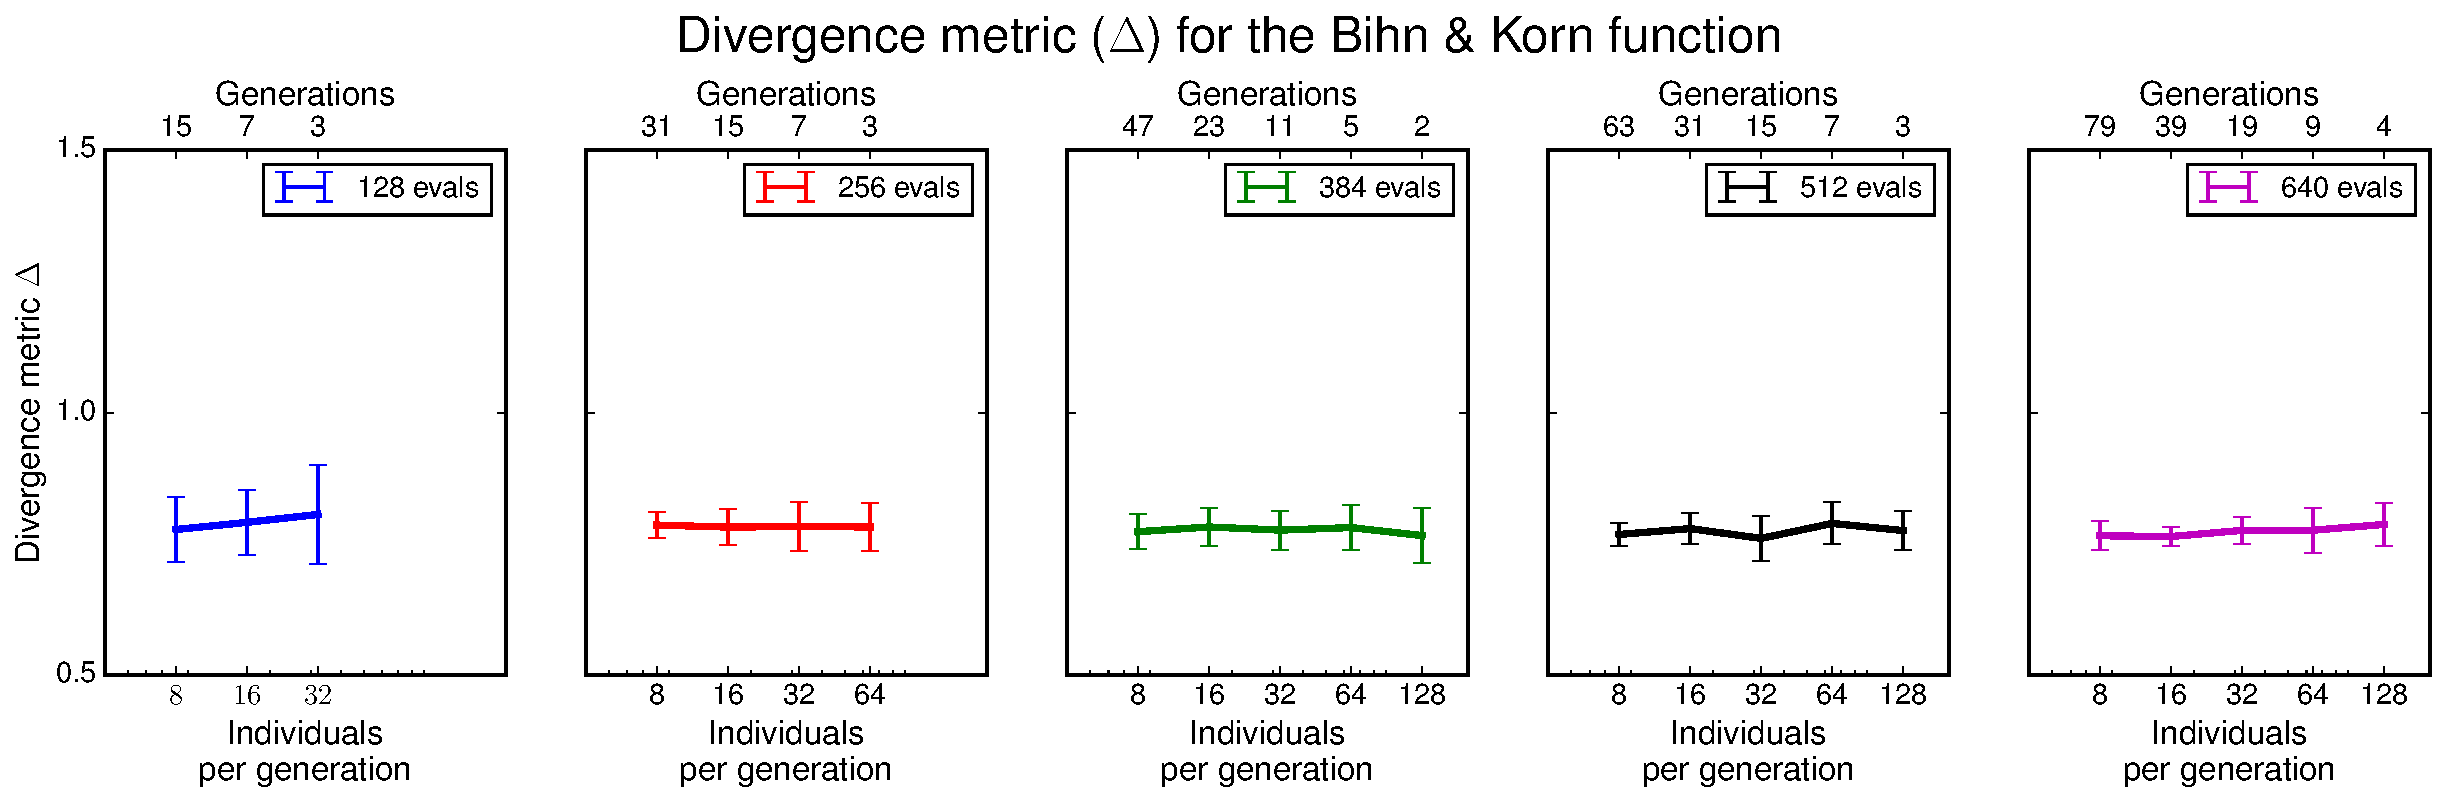
\includegraphics[width=\textwidth]{Figures/3/diverMetric_BK.pdf}
    \end{figure}
    \begin{figure}[h!]
        \centering
        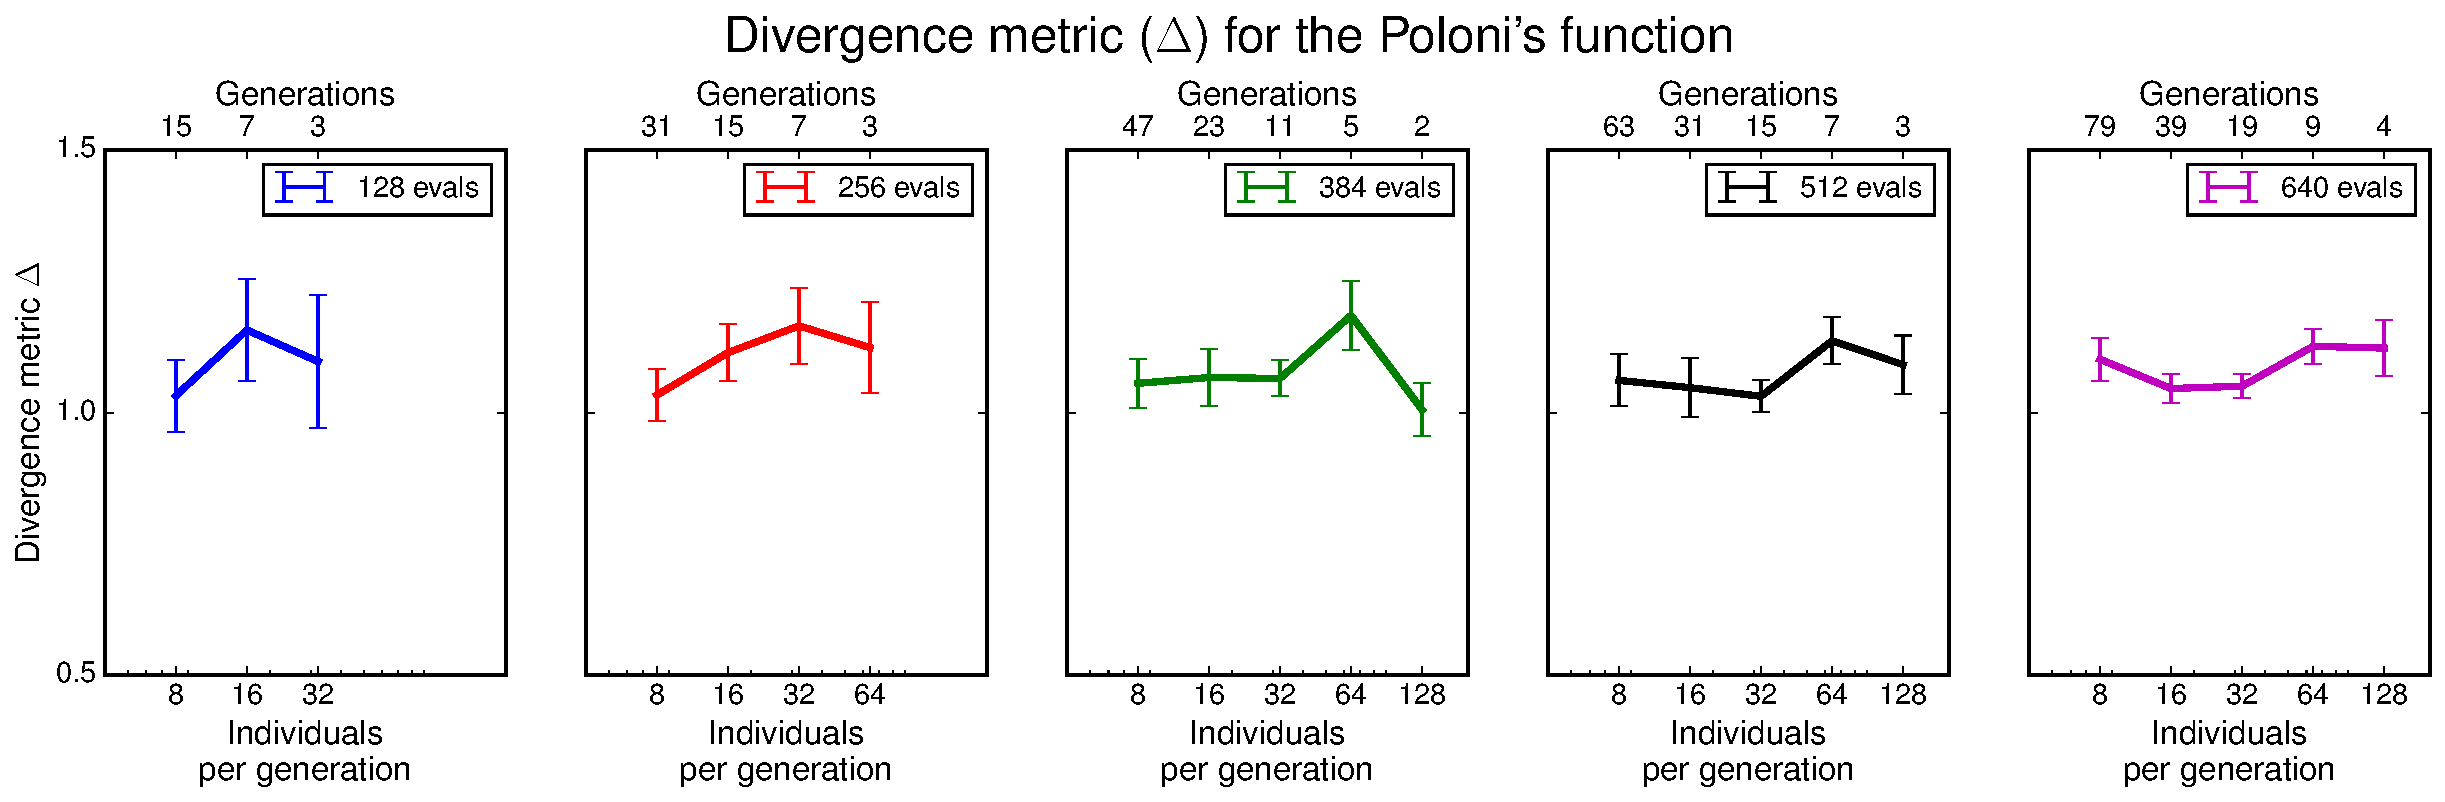
\includegraphics[width=\textwidth]{Figures/3/diverMetric_POL.pdf}
    \end{figure}
    \begin{figure}[h!]
        \centering
        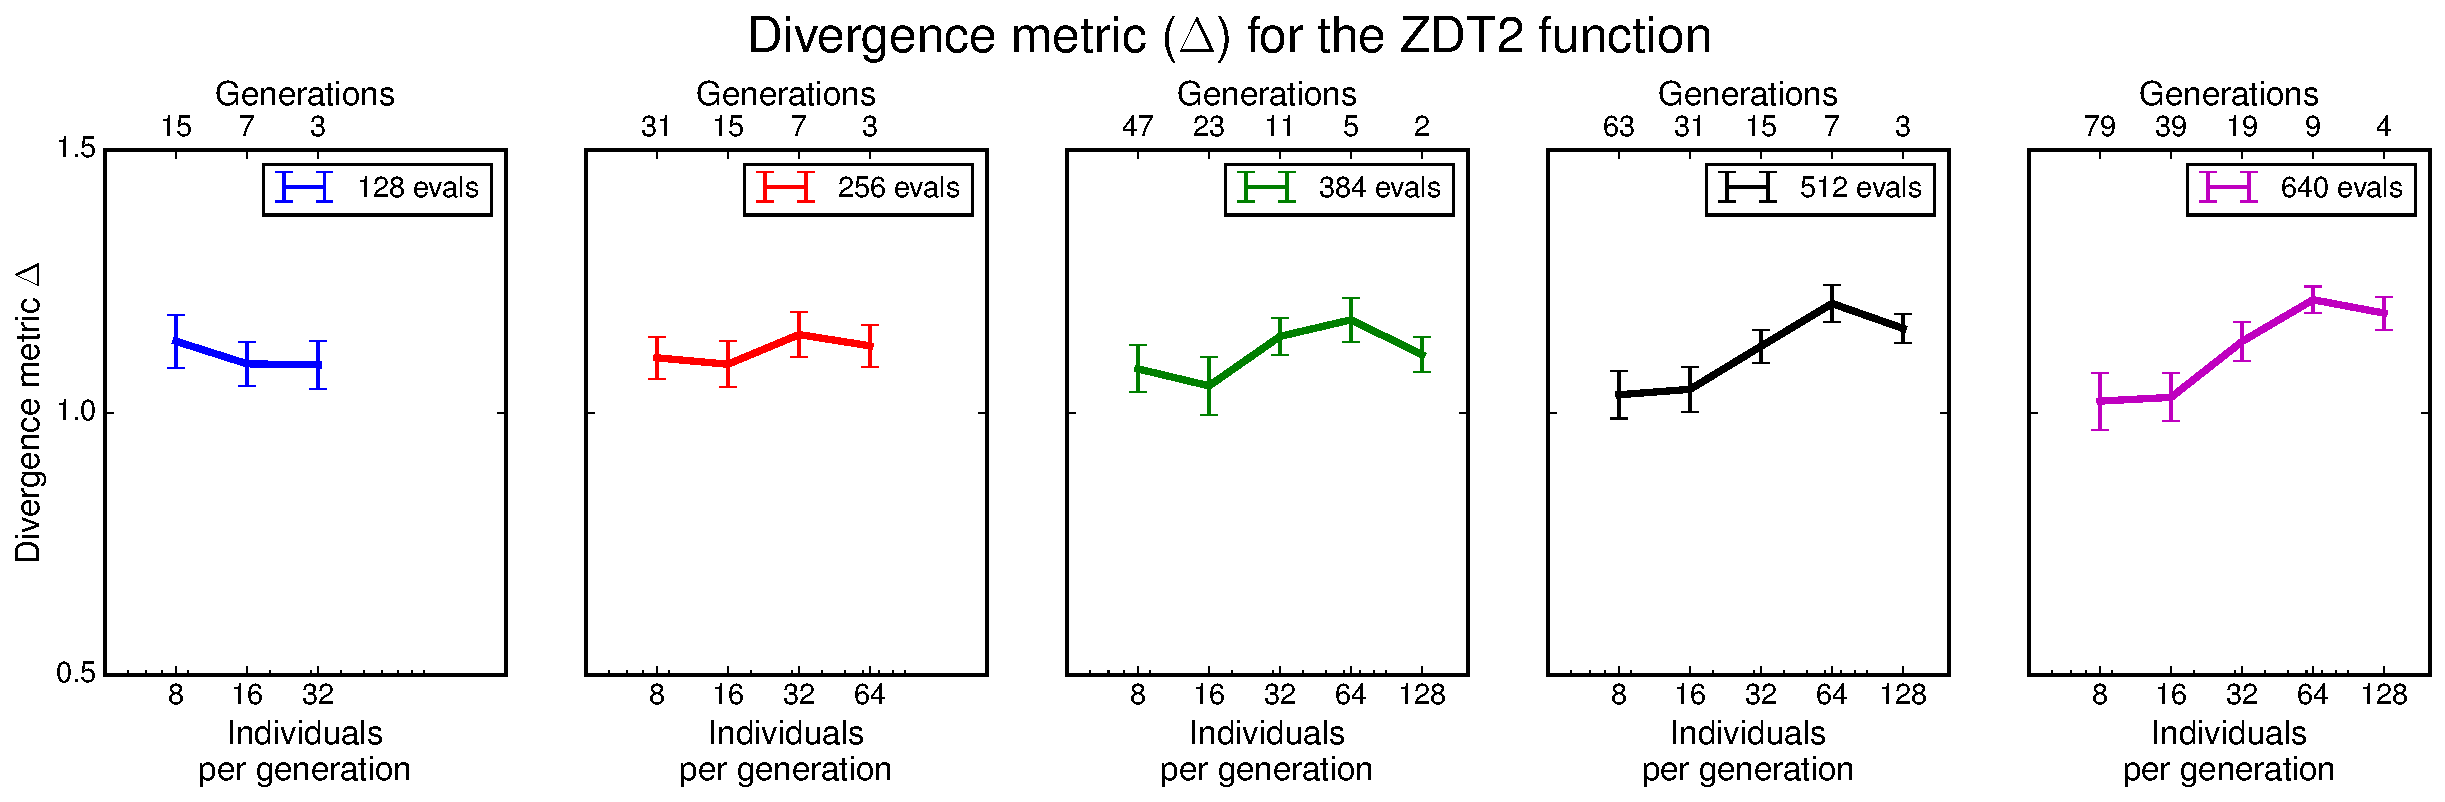
\includegraphics[width=\textwidth]{Figures/3/diverMetric_ZDT.pdf}
        \caption{Divergence metric for the three different test functions}
        \label{fig:diverMetric}
    \end{figure}

The convergence metric ($\Upsilon$) results are shown in Figure \ref{fig:convMetric}. In this case, there is a clear trend: the convergence to the True Pareto front increased with more individuals per generation that with more generations of smaller populations. It must be noted that the first figure in \ref{fig:convMetric} has different vertical limits. However, what is really important is the trend that the metric follow. The results for the ZDT2 function also reveal that the number of generations may be kept small but allowing the population to converge to a solution. Thus, creating a population of very large size and evaluating it just for 3 or 4 generations will not give accurate solutions. 

    \newpage
    
    \begin{figure}[h!]
        \centering
        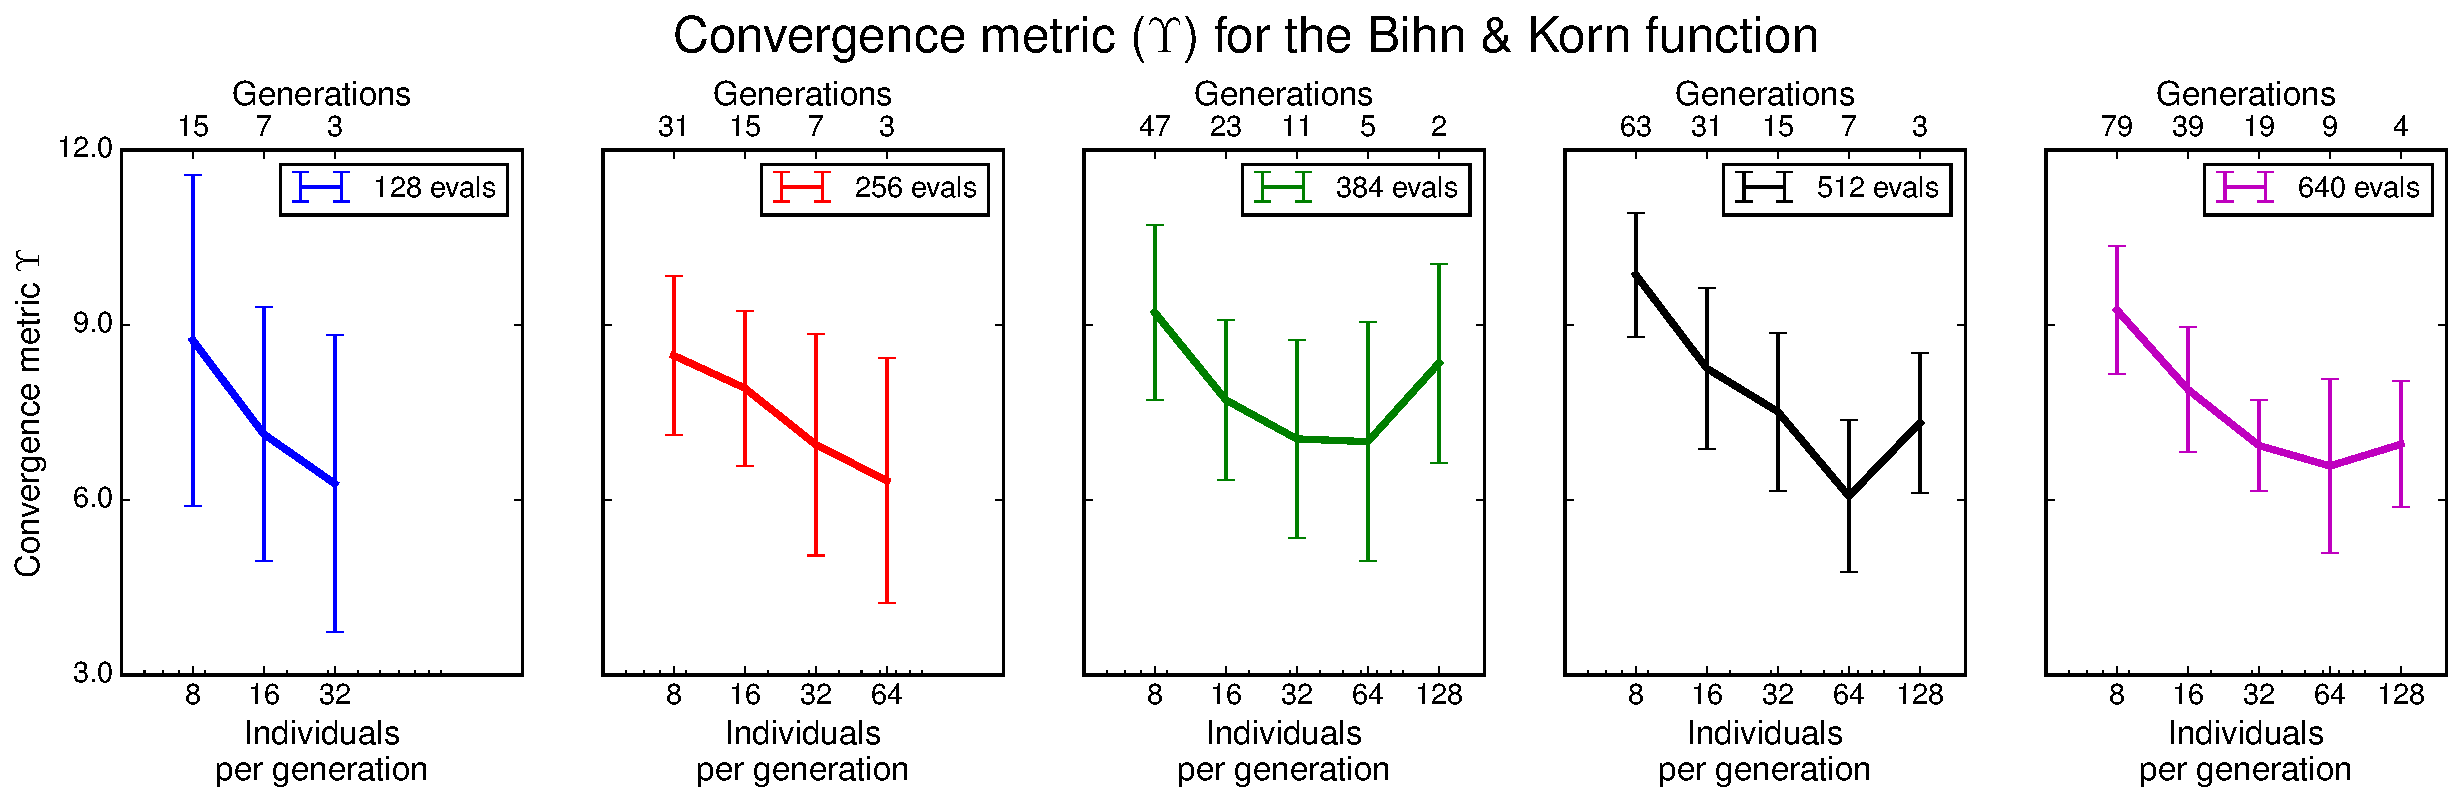
\includegraphics[width=\textwidth]{Figures/3/convMetric_BK.pdf}
    \end{figure}
    \begin{figure}[h!]
        \centering
        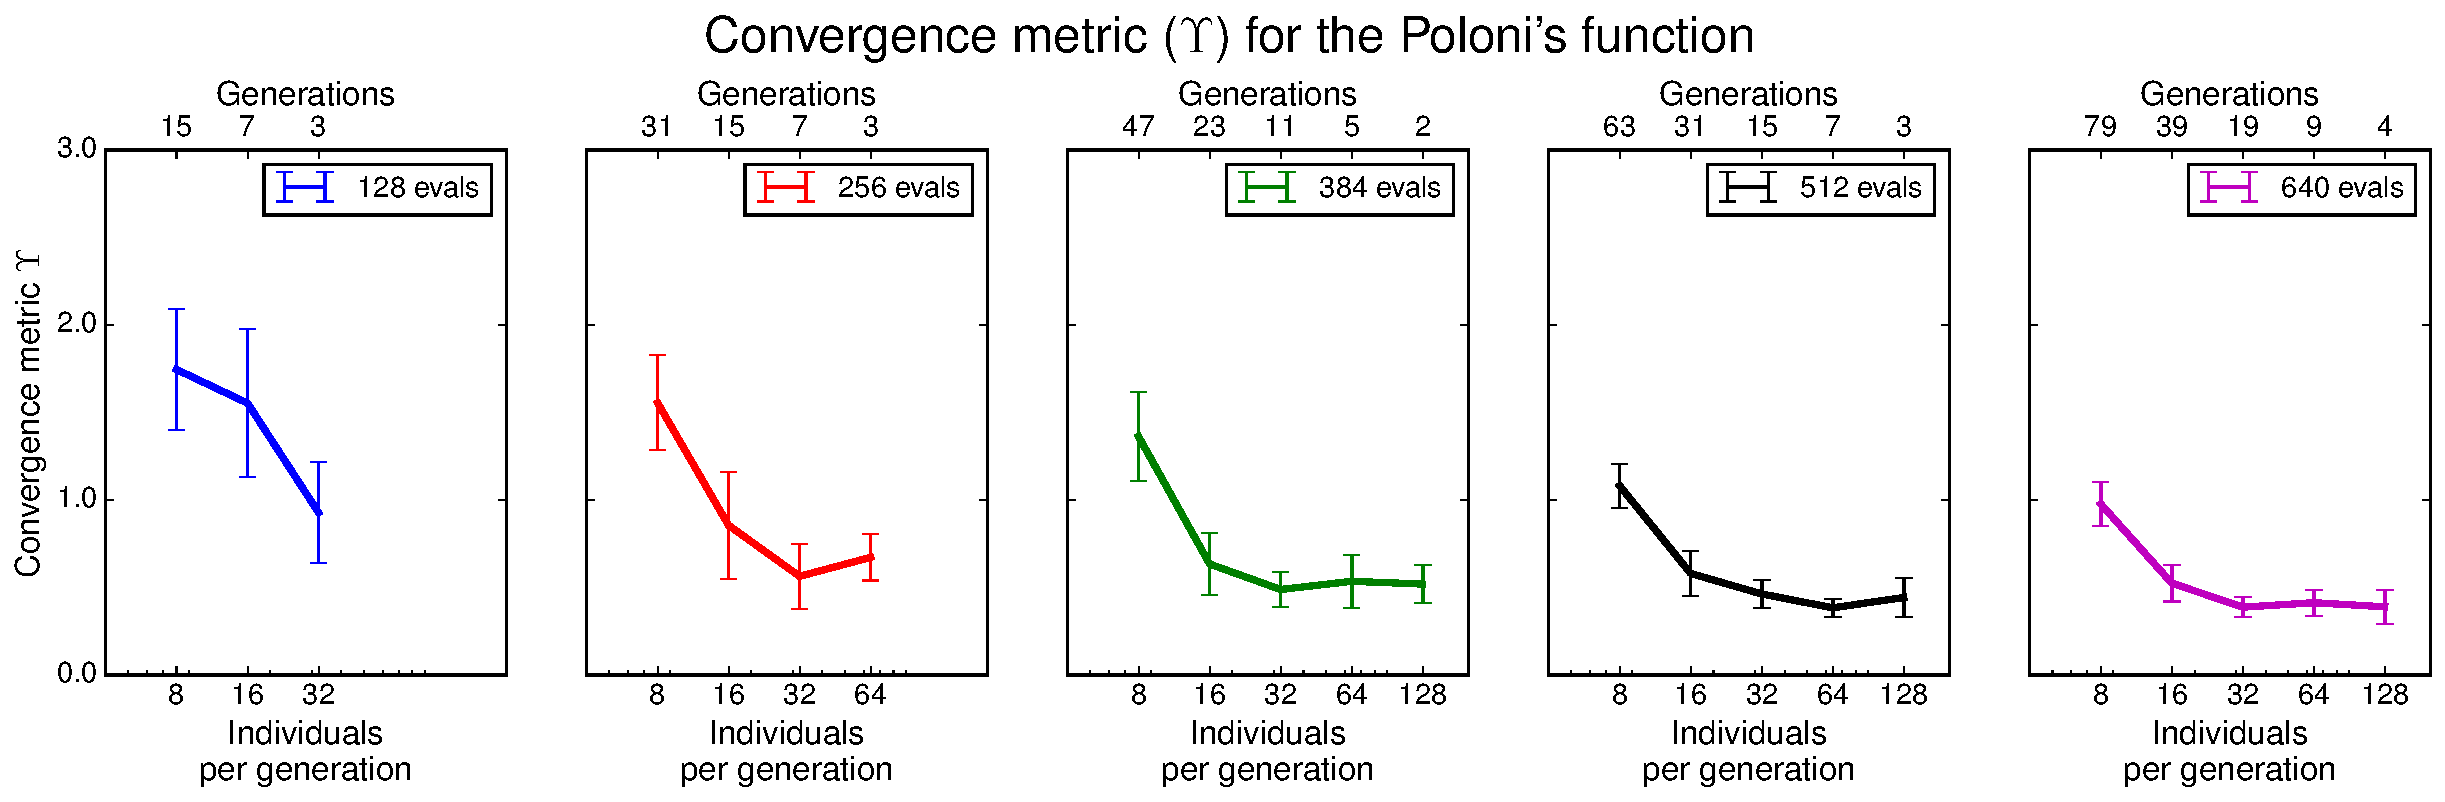
\includegraphics[width=\textwidth]{Figures/3/convMetric_POL.pdf}
    \end{figure}
    \begin{figure}[h!]
        \centering
        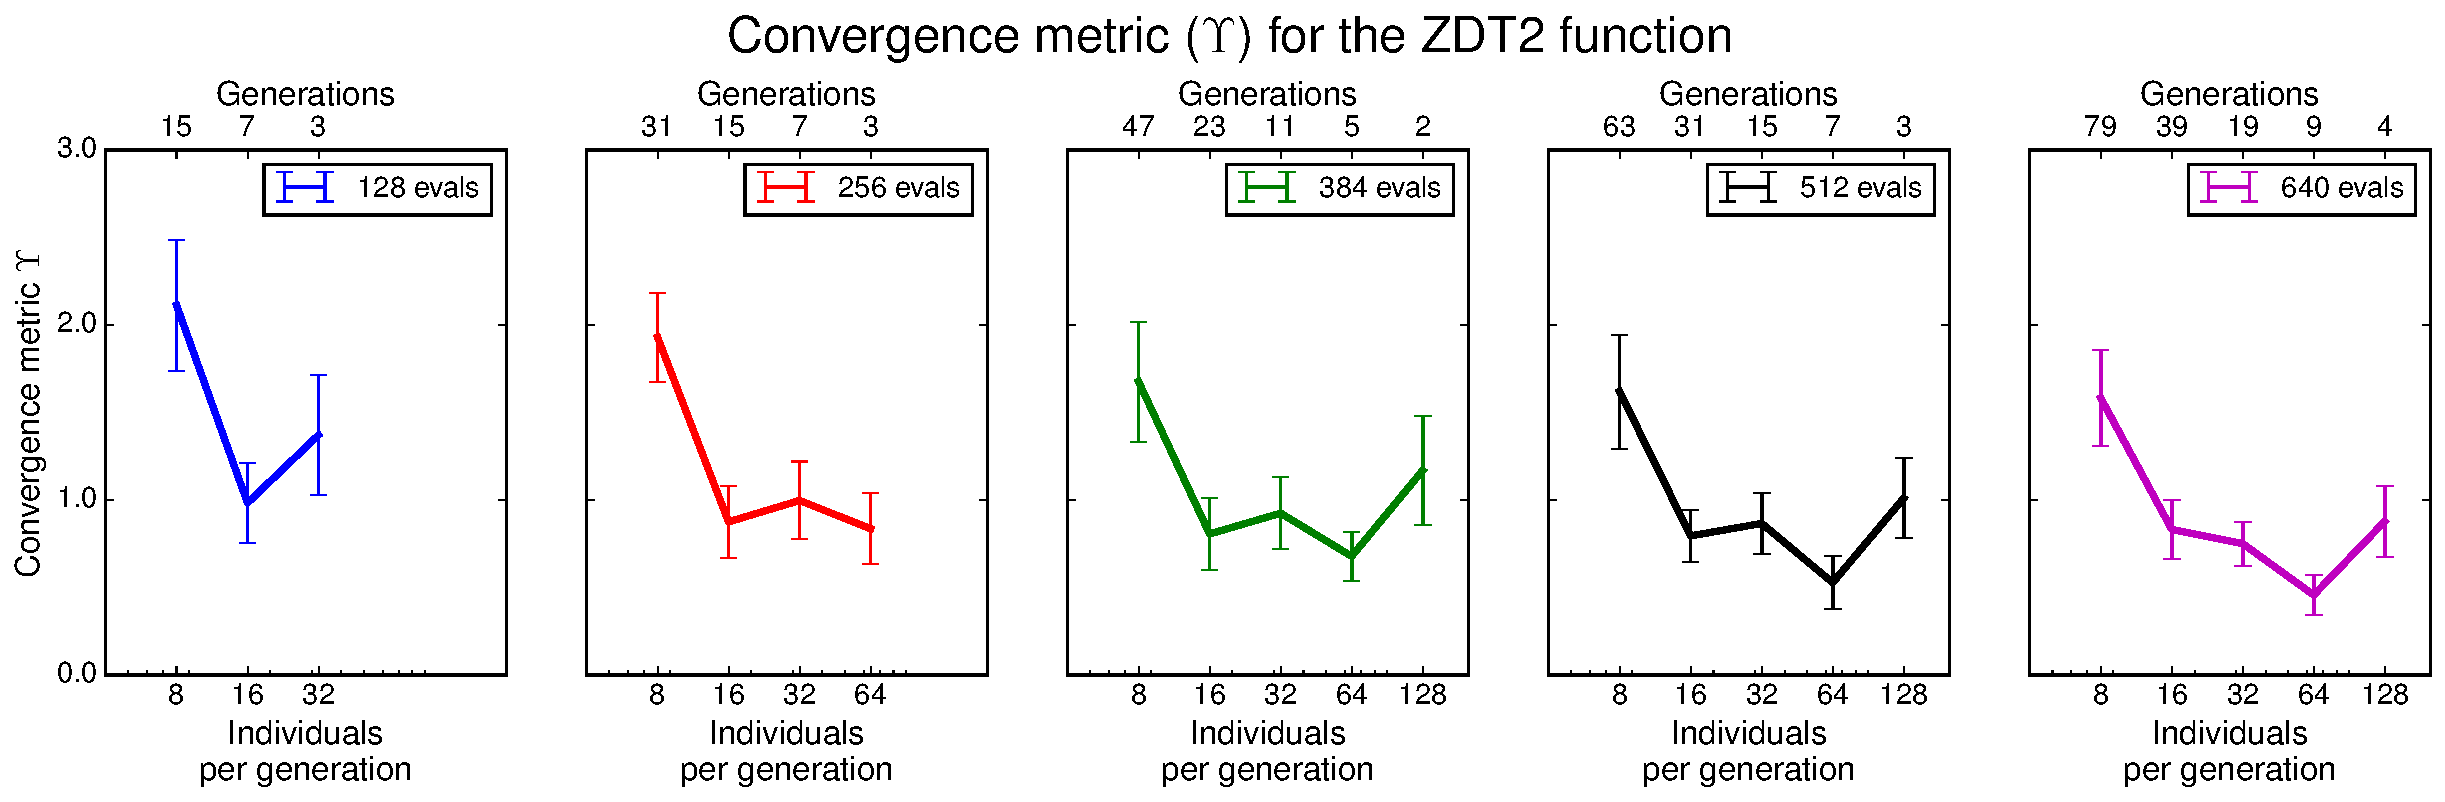
\includegraphics[width=\textwidth]{Figures/3/convMetric_ZDT.pdf}
        \caption{Convergence metric for the three different test functions}
        \label{fig:convMetric}
    \end{figure}
   
\newpage

\section{CFD cases}

In this subsection, different CFD setups will be presented and explained (showing the results in the following section). The code of the NSGA-II was implemented in Python for a two variable and two function case (although it may be easily upgraded to a higher number of variables and objective functions). The different individuals were generated from Python scripts that transformed the variables into a mesh or a configuration file for a case. Each individual has been simulated with OpenFOAM in a parallel fashion (using MPI for multiprocessor parallel computing). The results obtained from the simulation were analyzed with ParaView (in the \texttt{pvbatch} mode) or directly with Python to get the fitness value of each individual. With that fitness value, the genetic algorithm computed the next generation, sending it to OpenFOAM as before. All this loop was controlled with Bash scripting: from running the simulations and waiting for them to finish before sending the next set to calling the different scripts for every individual and generation. Only 2D cases were analyzed, although the procedure for 3D cases will be the same.

The workstation used to perform the different cases was a machine with 32 processors (Intel Xeon CPU E5-2650 @ 2.00GHz), 64 Gb of RAM memory and a 275 Gb SSD hard disk. The machine was running under Ubuntu 16.04 LTS, with OpenFOAM version 5.00, ParaView v5.4.0 and Python 3.6.4. The amount of data obtained after the simulation process almost fill the whole solid state drive, so listing the whole code is unfeasible. However, the basic files for performing the different cases are available in GitHub (\url{https://github.com/jlobatop/GA-CFD-MO}) as well as the code and Jupyter notebooks developed along the process of this thesis. 

\subsection{Suppression of cylinder vortex oscillations}

The first one of the cases is the flow around a cylinder. Although cylinders may seem a very simple case, the results obtained for a cylinder may be extrapolated and used in other cases, such as airfoils. Vortex shedding is a phenomenon that happens when the equilibrium flow around a cylinder suffers a Hopf bifurcation (instability caused by background distances) and the flow enters into a new equilibrium which is time-periodic (at the Strouhal frequency) \cite{sengupta2010dynamical}. This is a major problem when mixing structural behavior and flow dynamics, because if the Strouhal frequency matches the natural frequency of the structure, the consequences may be catastrophic because an excited natural frequency usually leads to unstable behavior of the structure \cite{green2006failure}.

\newpage

There are a lot of ways of suppressing the vortex shed oscillations that are present in the wake of the cylinder. The methods are classified in passive and active, depending if they are looped with some kind of feedback from the state of the system. Vortex shedding may be controlled with a lot of techniques, where the most common ones are magnetic field, rotary oscillations, secondary flow and surface roughness. In this analysis, a passive flow control with a secondary flow will be used. Instead of using a simple blowing jet, a blowing and suction jet will be installed in the rear part of the cylinder. Using a sinusoidal wave that introduces and extracts momentum (instead of a pulse jet that only introduces momentum) avoid issues related to mass conservation in the CFD simulation \cite{rashidi2016vortex}.

\subsubsection*{Case setup}

As said, the flow control will be performed with a sinusoidal wave type of function that depends on two variables: the amplitude ($A$ or $v$ given that the variation in momentum insertion is performed with changes in the velocity) and the frequency ($f$). The initialization of the flow control is performed once the von Karman vortex shedding is already developed, so the phase shift of the sinusoidal wave is fixed. The objective of the optimization is to minimize the force oscillations in both the horizontal and vertical axis. In order to quantify the oscillations, different approaches were considered. The output of the OpenFOAM solver returns a force-time data file that contains the forces that the cylinder is suffering. In order to capture the amplitude of the data obtained, a Fourier transform was at first considered. The amplitude values are very small so the \texttt{FFT} (Fast Fourier Transform) implemented in Python did not work properly. Computing the root mean square (RMS) error was also viewed as a possible approach. The RMS for a data set is defined as \cite{bissell1992digital}:

\begin{equation}
    x_{rms}=\sqrt{\dfrac{1}{n}\left( x_1^2 + x_2^2 + ... + x_n^2 \right)}
\end{equation}

\begin{equation}
    x_{rms}^2=\overline{x}^2+\sigma_x^2=\overline{x^2}
\end{equation} 
where $\bar{x}$ is the mean and $\sigma_x$ is the standard deviation. The problem that this metric has is that it cannot go to zero because the mean $\overline{x}$ will not go to zero given that there is only one exit in the rear part and the force exerted is not compensated with a front membrane (having that $\overline{x}\neq 0$). Thus, scenarios with small forces and large oscillations will have the same RMS value of larger forces but zero oscillations cases. 

The metric that better represent the problem is the standard deviation $\sigma$. Computing it in the last $n$ cycles (where $n$ depends on the complete cycles that have been captured in the simulation), an oscillatory force will only have $\sigma=0$ if the amplitude of the oscillations is zero. Thus, the algorithm will try to minimize $\sigma_Y$ and $\sigma_X$ for a sum of the pressure and viscous forces.

The genetic algorithm setup was done with 64 individuals in the first generation and just 10 individuals for each other generation. A 6 generation limit was also established. These limits may be very strict but they are chosen for computational resources limitations. A more powerful study may be performed, surely achieving more accurate solutions. The search domain is $A\in[0.01,2]$ and $f\in[0.01,\pi/2]$. The solver used is \texttt{pimpleFoam}, which is an incompressible solver for transient cases. The maximum time of simulation was 150 seconds. Newtonian transport model with laminar turbulence modeling was chosen. The case was done in a non-dimensionalized fashion, with a density value of $\rho=1 kg\cdot m^{-3}$, a viscosity value of $\nu=1\times 10^{-5} m^2\cdot s^{-1}$, and a cylinder diameter of $1\ m$ facing a flow at a velocity of $1\ m\cdot s^{-1}$. This values give a Reynolds number of $Re = 100,000$. Vortex shedding at this Reynolds number happens to occur in a turbulent way. Most of the schemes were chosen as \texttt{linear} and the time differentiation scheme was chosen to be \texttt{backward}. The real mesh can be seen in Figure \ref{fig:cylMeshSChematicsPF} and the mesh details are shown in Figure \ref{fig:cylMeshSChematics}.


    \begin{figure}[h!]
        \centering
        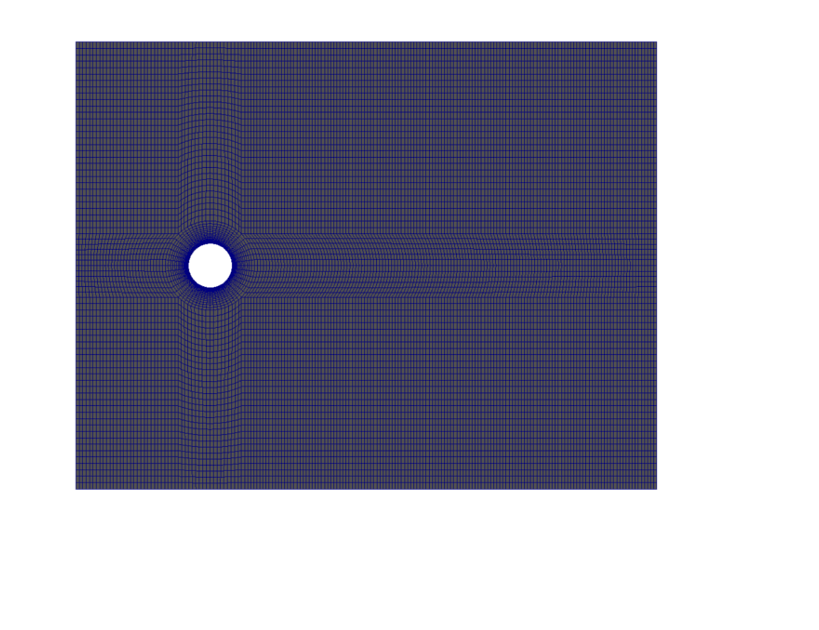
\includegraphics[width=0.8\textwidth]{Figures/3/cylinderMeshPF.png}
        \caption{Picture of the mesh for the cylinder case}
        \label{fig:cylMeshSChematicsPF}
    \end{figure}

\newpage

    \begin{figure}[h!]
        \centering
        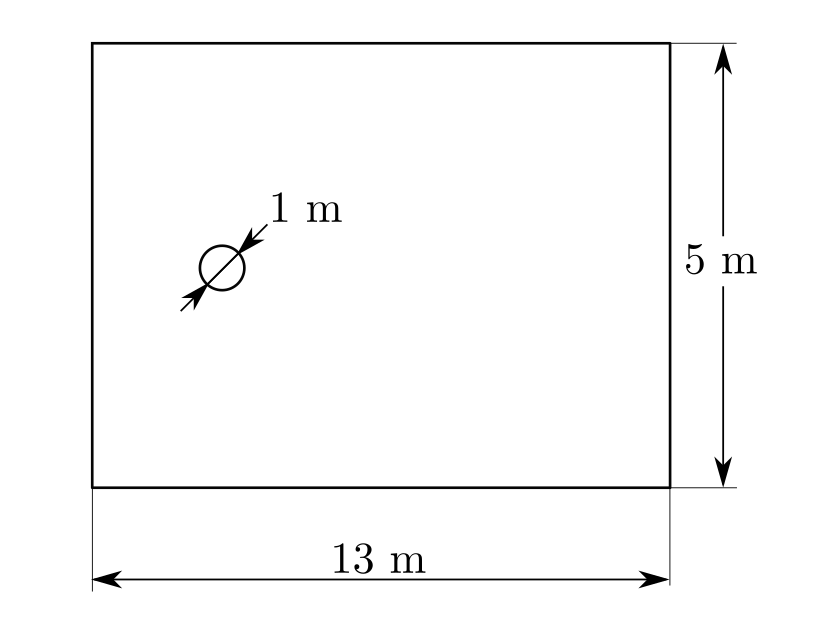
\includegraphics[width=0.6\textwidth]{Figures/3/cylinderMesh.png}
        \caption{Schematics of the mesh for the cylinder analysis}
        \label{fig:cylMeshSChematics}
    \end{figure}


The boundary conditions imposed in the different faces are listed with an exploded view of the mesh. 

  
      \begin{table}[h!]
        \centering
        \caption{Boundary conditions for the cylinder case}
        \label{fig:tableCylBC}
        \begin{tabular}{cc}
        \multicolumn{2}{c}{\textbf{Inlet (yellow)}}          \\
        \hline
        $U$                    & \texttt{fixedValue (1 0 0)}           \\
        $p$                     &  \texttt{zeroGradient}          \\
        & \\
        \multicolumn{2}{c}{\textbf{Outlet (green)}}          \\
        \hline
        $U$                    & \texttt{zeroGradient}           \\
        $p$                     &  \texttt{fixedValue 0}          \\
        & \\
        \multicolumn{2}{c}{\textbf{Flow control membrane (grey)}}      \\
        \hline
        $U$                    & \begin{tabular}{c}
             \texttt{uniformFixedValue} \\
             \texttt{(tableFile)}
        \end{tabular}           \\
        $p$                     &  \texttt{zeroGradient}          \\
        & \\
        \multicolumn{2}{c}{\textbf{Upper/Lower (grey)}}      \\
        \hline
        $U$                    & \texttt{symmetry}           \\
        $p$                     &  \texttt{symmetry}          \\
        & \\
        \multicolumn{2}{c}{\textbf{Cylinder (red)}}      \\
        \hline
        $U$                    & \texttt{fixedValue (0 0 0)}           \\
        $p$                     &  \texttt{zeroGradient}          \\
        & \\
        \multicolumn{2}{c}{\textbf{Front/Back (white)}}      \\
        \hline
        $\texttt{*}$                    & empty \\
        \end{tabular}
        \end{table}

\newpage

     \begin{figure}[h!]
        \centering
        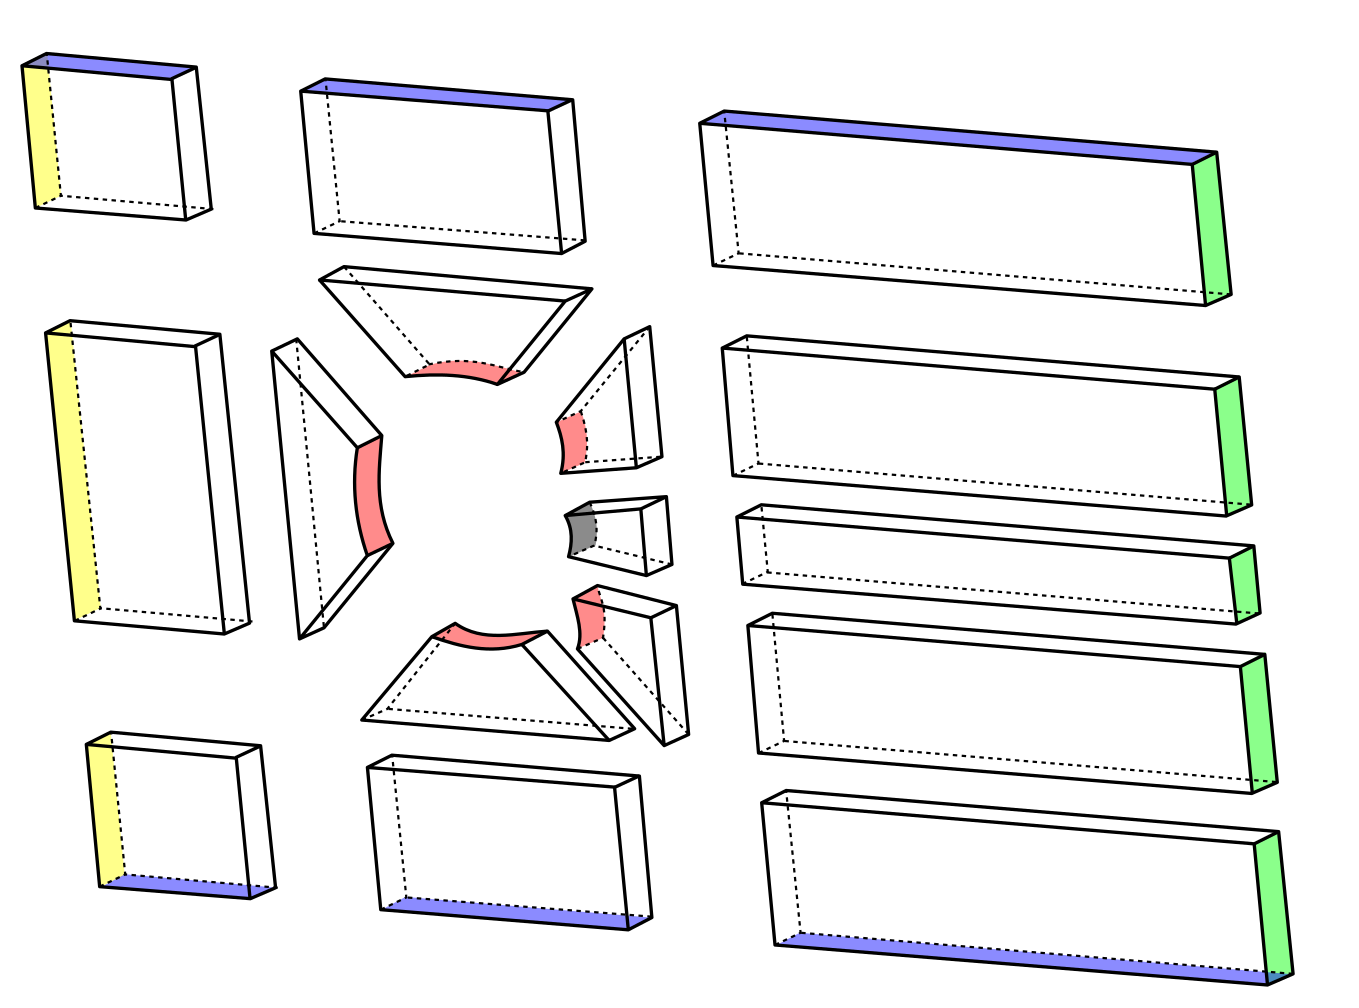
\includegraphics[width=0.55\textwidth]{Figures/3/cylinderMeshBC.png}
        \caption{Exploded view of the mesh for the cylinder case}
        \label{fig:cylBC}
    \end{figure}


\subsection*{Processor convergence}

Apart from the typical mesh convergence studies, the processor convergence type of analysis is critical in this highly parallelizable cases. One simulation may be divided for a different number of processors, having that time reaches a minimum in some number of processors. Total simulation time is the sum of the simulation time, case decomposition time and case reconstruction time. For 1 processor there are no decomposition nor reconstruction times, so the total time is the same as the simulation time. 

     \begin{figure}[h!]
        \centering
        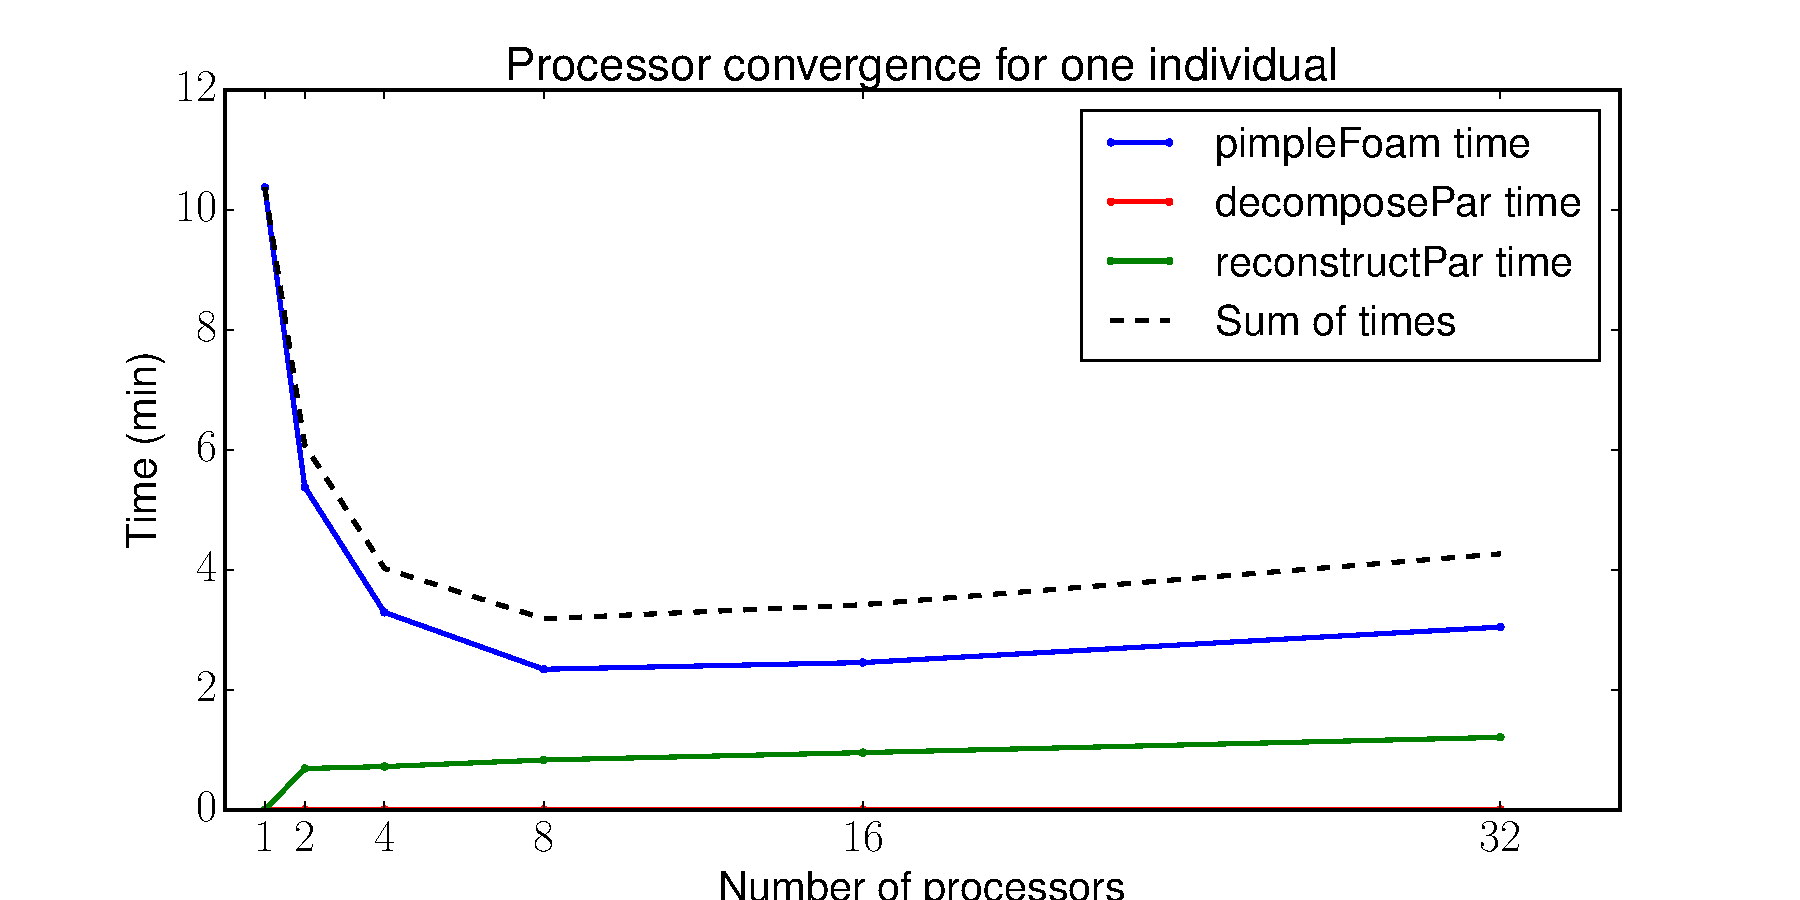
\includegraphics[height=0.35\textheight]{Figures/3/procConv_1ind.pdf}
        \caption{Processor convergence for 1 individual}
        \label{fig:procConvergenceCyl}
    \end{figure}

\newpage

The results of the processor convergence in Figure \ref{fig:procConvergenceCyl} shown that using $8$ processor gives the fastest results. However, when applying genetic algorithms or another population-based algorithm, there are a lot of simulations that might be performed at the same time. If each individual is computed in 1 processor (and constraining the problem to a 32-processors machine), then 32 individuals may be computed at the same time. If each individual is simulated in 2 processors, only 16 individuals may be run at the same time (so if each population is formed by 32 individuals, 16 must be simulated first and 16 once the latter have finished). If each individual is run in 4 processors, only 8 individuals may be simulated at the same time, sending the population into 4 groups of 8. 


If the sum of times from one individual is multiplied by the divisions that must be made to a generation of $32$ individuals for simulating the whole population, an estimation of the simulation time is obtained. Nevertheless, the real times were computed and plotted in Figure \ref{fig:genProcConvergenceCyl}, seeing that there is a difference between the actual values and the estimated ones (probably due to the fact that there are computational resources that were not affected in the one individual simulation times).  

     \begin{figure}[h!]
        \centering
        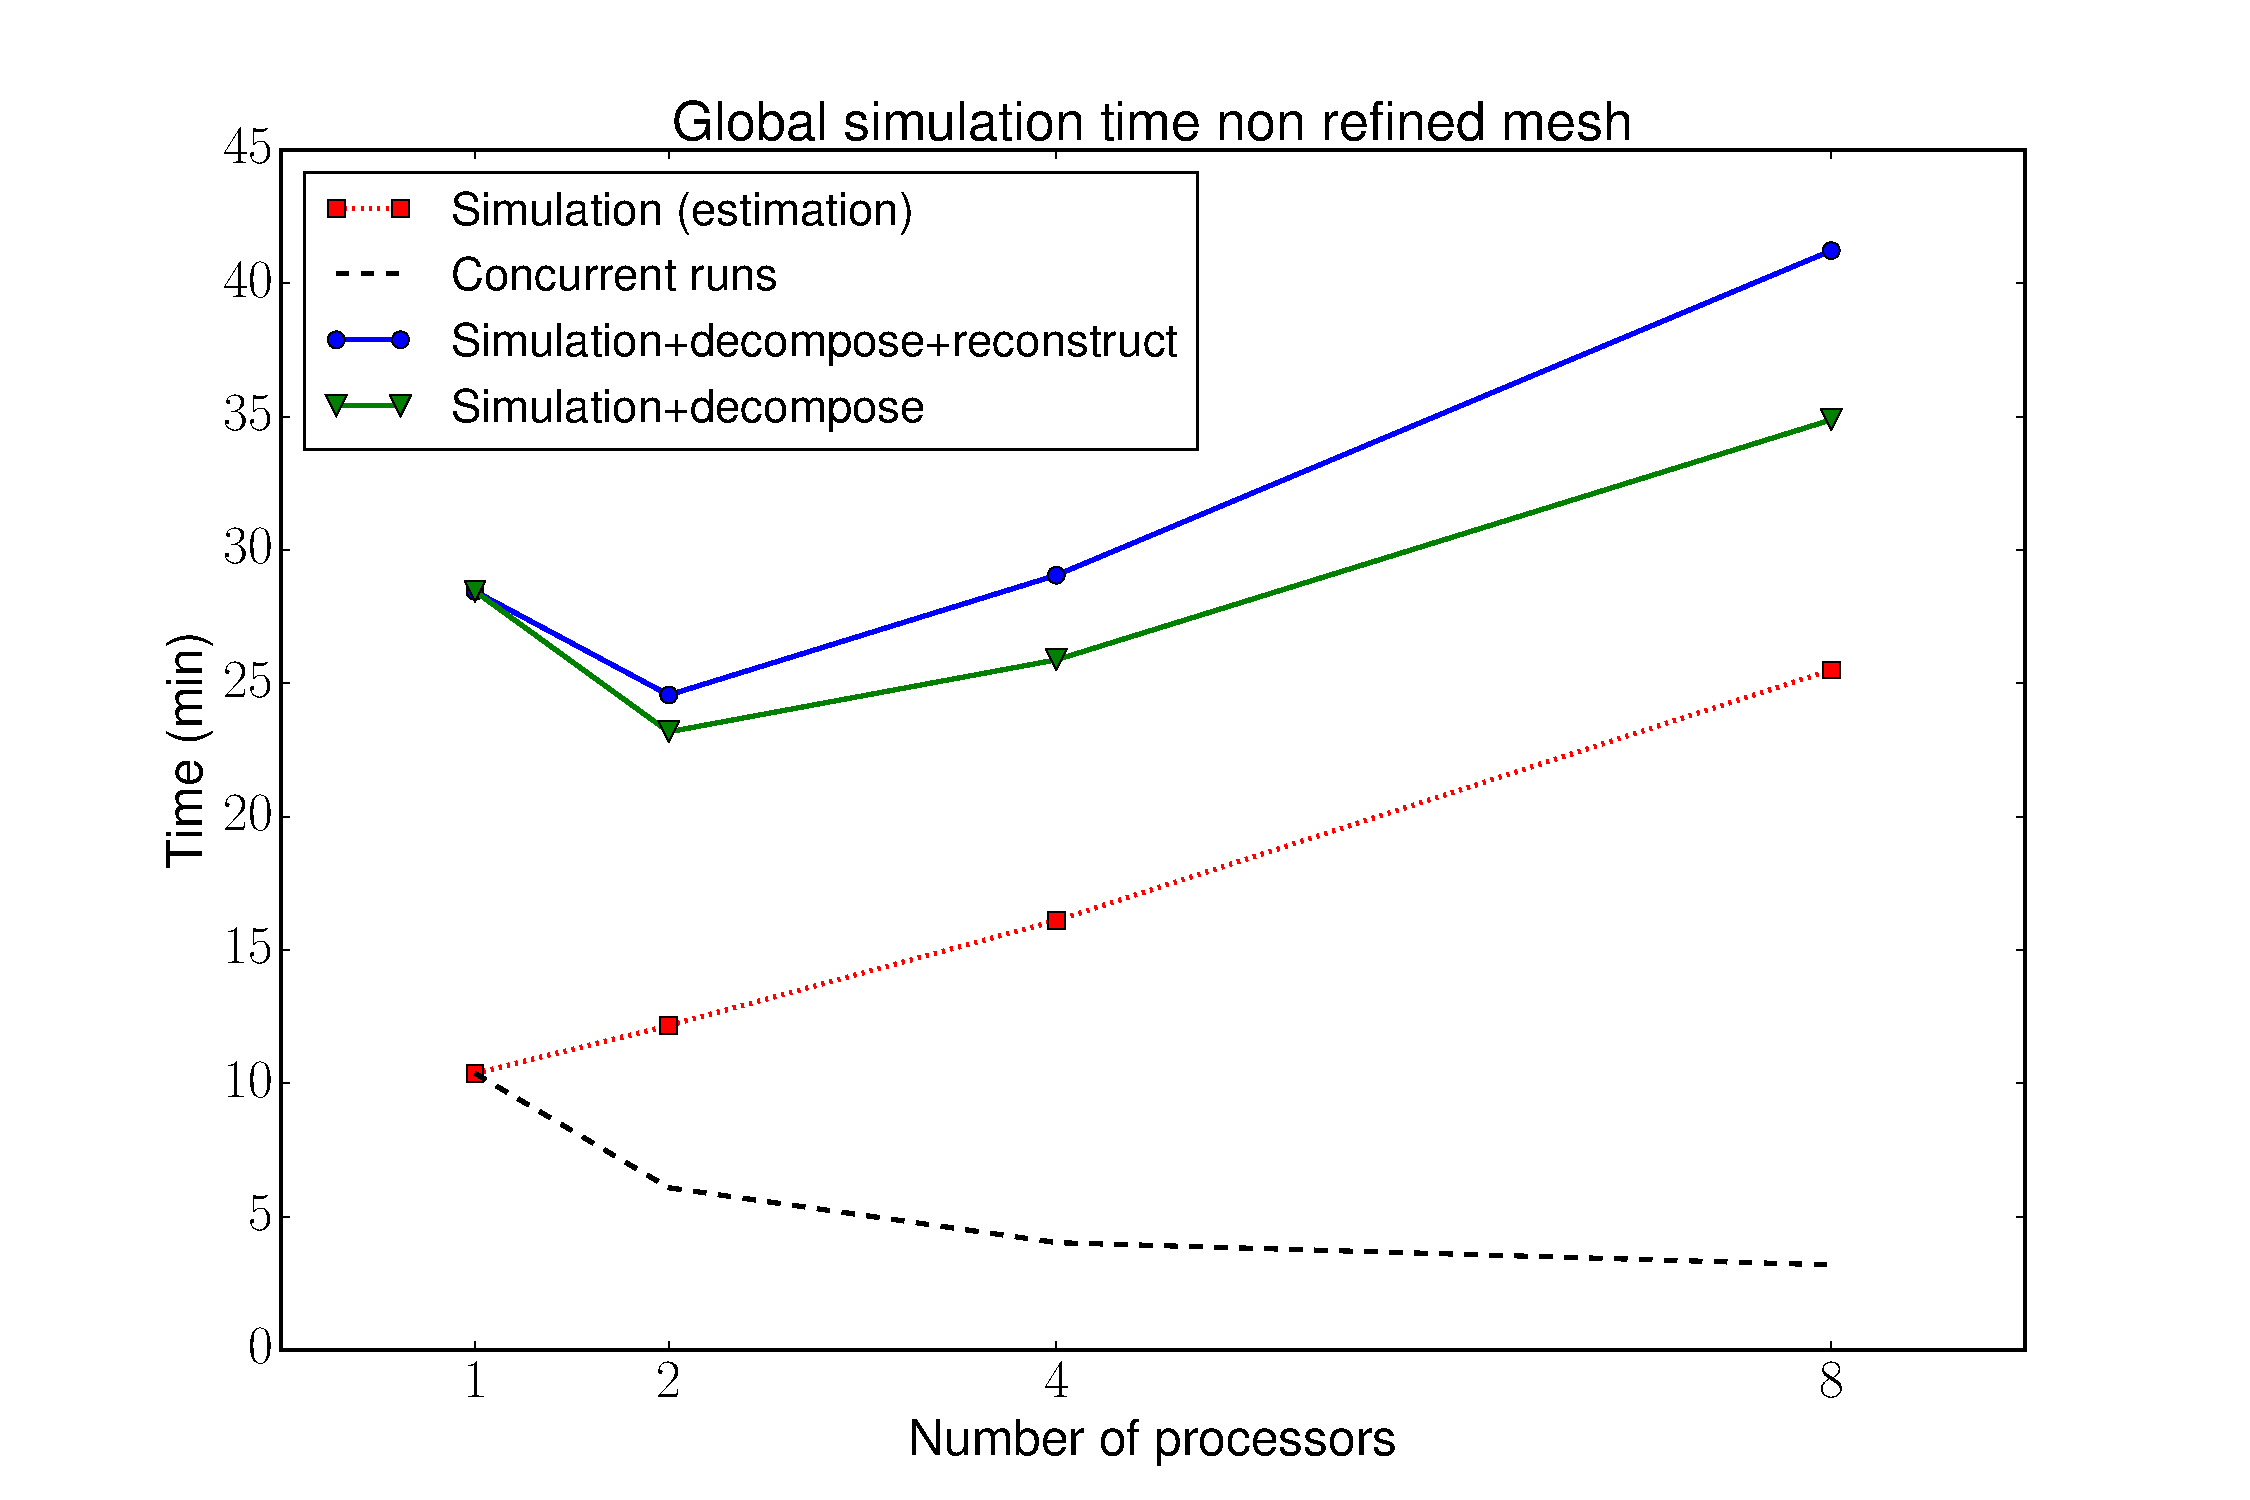
\includegraphics[width=0.85\textwidth]{Figures/3/procConv_1gen2.pdf}
        \caption{Processor convergence for a 32 individual population}
        \label{fig:genProcConvergenceCyl}
    \end{figure}

The reconstructed time has been separated from the decomposition time because in order to analyze the results it is not strictly necessary to reconstruct the case. This does not make any difference because, for all the cases, the most optimal configuration is to use 2 processors. 

\newpage

\subsection{Inlet of diffuser geometry}

Optimizing the inlet of a diffuser is the first step for increasing the efficiency and performance of the engine as a whole. Inlet diffuser geometry is a well-known problem that has been studied in multiple approaches \cite{djebedjian2004two}, \cite{schmandt2011diffuser}. However, there are a lot of shapes in which the inlet may be optimized, e.g., if multiple variables are analyzed, the shape may be parametrized with splines or with control nodes. For simplification purposes, in this study the shape was computed with two values: a length ($L$) and an angle ($\theta$), which are the search space variables. The function space is formed by the total pressure ratio (computed between the total pressure in the outlet of the diffuser and the freestream total pressure) and by the Mach number in the diffuser outlet. Both values will be maximized. The first one seems evident to maximize: total pressure ratio is related to entropy generation and the lower the entropy generation, the better. The maximization of the Mach number in the outlet of the diffuser may be useful in supersonic combustion engines, where there is not turbomachinery and the flow may enter at supersonic speeds to the diffuser \cite{cain2002review}. 

\subsubsection*{Case setup}

In this case, instead of varying the flow conditions as before, the optimization will be performed to the mesh. Thus, each combination of $L$ and $\theta$ will have an associated mesh, having all the meshes with the same boundary conditions of $M_\infty$, $p_\infty$ and $T_\infty$. A combination of the two may be performed, having, for example, $L$ and $Ma$ as the search space variables to maximize both the pressure ratio and the Mach number at the diffuser outlet (having the problem of the moving inlet of the SR-71 Blackbird).  Both the Mach number and the total pressure ratio are computed in Python with values extracted from Paraview. The genetic algorithm used 32 individuals per generation and 6 generations limit. This simulation was performed with a compressible steady state solver (\texttt{rhoSimpleFoam}) with 2500 maximum iterations, where the residuals were stable. The turbulence modeling was done with a $k-\epsilon$ model under Newtonian fluid and perfect gas assumptions. The freestream velocity was $u_\infty = 590\ m\cdot s^{-1}$ which for a temperature of $T_\infty=216\ K$ yields a Mach number of $Ma=2$, freestream pressure was $P_\infty=19930\ Pa$ which corresponds to a altitude of $12\ km$, viscosity was $\nu=1\times 10^{-5} m^2 \cdot s^{-1}$ and the density $\rho=0.31\ kg \cdot m^{-3}$. $k$, $\epsilon$, $\nu_t$ and $\alpha_t$ were chosen based on the tutorials in the OpenFOAM library. The Reynolds number for this case will vary depending on both the horizontal length $L$ and the inclination angle $\theta$, but it will be located near the $Re \sim 10^6-10^7$ range.

\newpage

The geometry of the mesh is sketched in Figure \ref{fig:diffuserMesh}, having some fixed distances for all possible individuals and some variable dimensions: $L$ and $\theta$. Fixed distances will constrain the possible dimensions that the step may have and they are necessary to avoid having a completely undefined problem. Python took each combination of $L$ and $\theta$, created a \texttt{blockMeshDict} with the corresponding dimensions and then run the file to get the mesh. 

     \begin{figure}[h!]
        \centering
        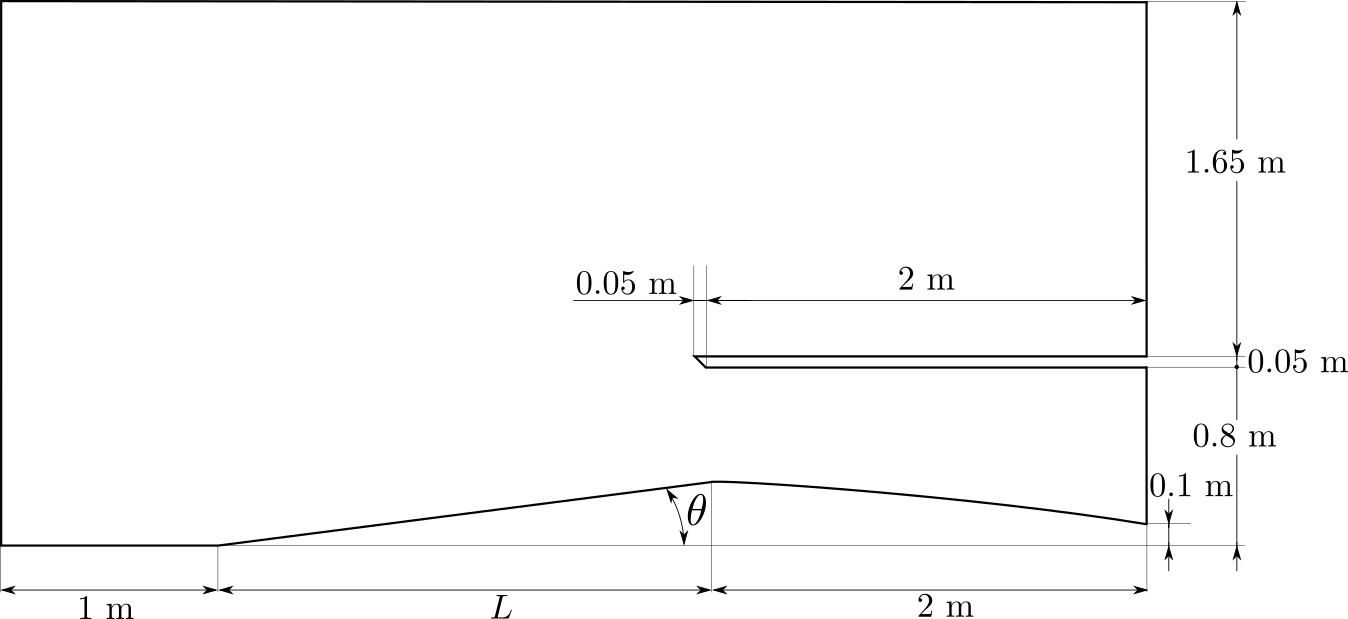
\includegraphics[width=0.85\textwidth]{Figures/3/diffuserMesh.png}
        \caption{Schematics of the mesh for the diffuser mesh}
        \label{fig:diffuserMesh}
    \end{figure}

One possible set of values $L-\theta$ returned the mesh shown in Figure \ref{fig:diffuserMeshPF}. It can be seen that the grading of the mesh is concentred in some zones while other zones have a more coarse grid. Given that \texttt{blockMesh} uses hexahedral blocks, the refinement must be performed along the dimensions of the hexahedral. This is a 2D case so in the spanwise direction $z$ there is only one cell (not shown in the picture).

     \begin{figure}[h!]
        \centering
        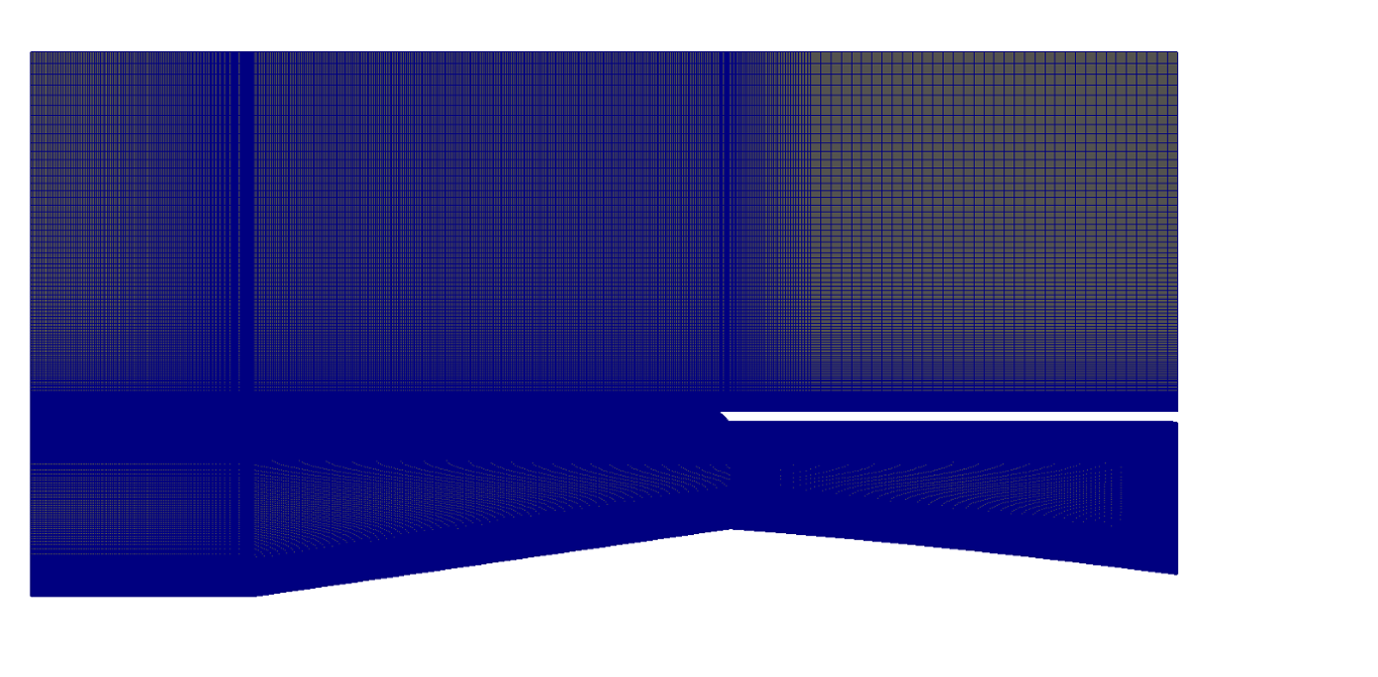
\includegraphics[width=0.86\textwidth]{Figures/3/diffuserMeshPF.png}
        \caption{Picture of the mesh for diffuser case (random $L$ and $\theta$)}
        \label{fig:diffuserMeshPF}
    \end{figure}
    
   \newpage
   
   As it has already been mentioned, the fixed dimensions of the mesh will bound the possible values that $L$ and $\theta$ take. The heights of $0.1\ m$ and $0.8\ m$ inside the diffuser will constraint the maximum and the minimum value of $\theta$ for each $L$. There is also $\theta^{phys}_{max}$ given by the attached oblique shock wave theory. It will only depend on the value of $M_\infty$, having a maximum angle limitation independent of the length $L$. Finally, a maximum length $L_{max}$ was fixed in order to avoid unrealistic lengths of the step.
      
     \begin{figure}[h!]
        \centering
        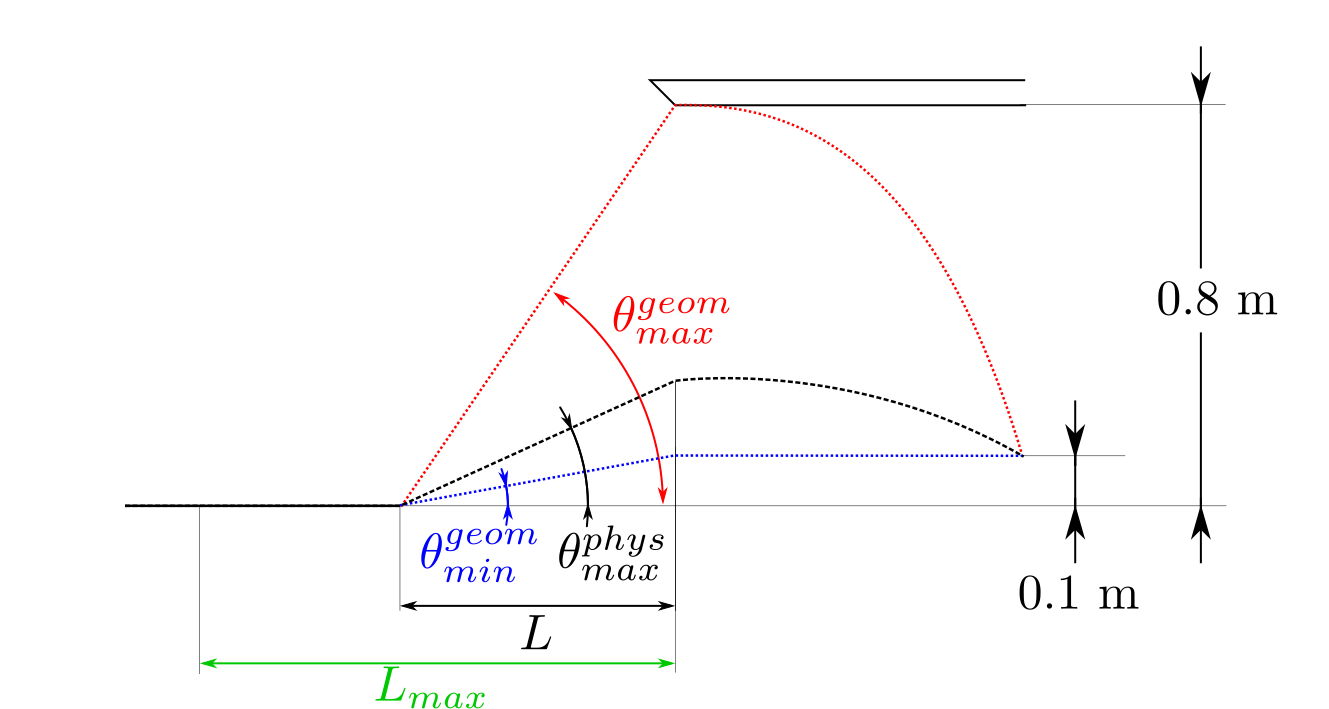
\includegraphics[width=0.85\textwidth]{Figures/3/diffuserConst4.png}
        \caption{Constraints for the diffuser case}
        \label{fig:diffuserConstr}
    \end{figure}

The search space is located in the grey zone (Figure \ref{fig:searchSpace}):

     \begin{figure}[h!]
        \centering
        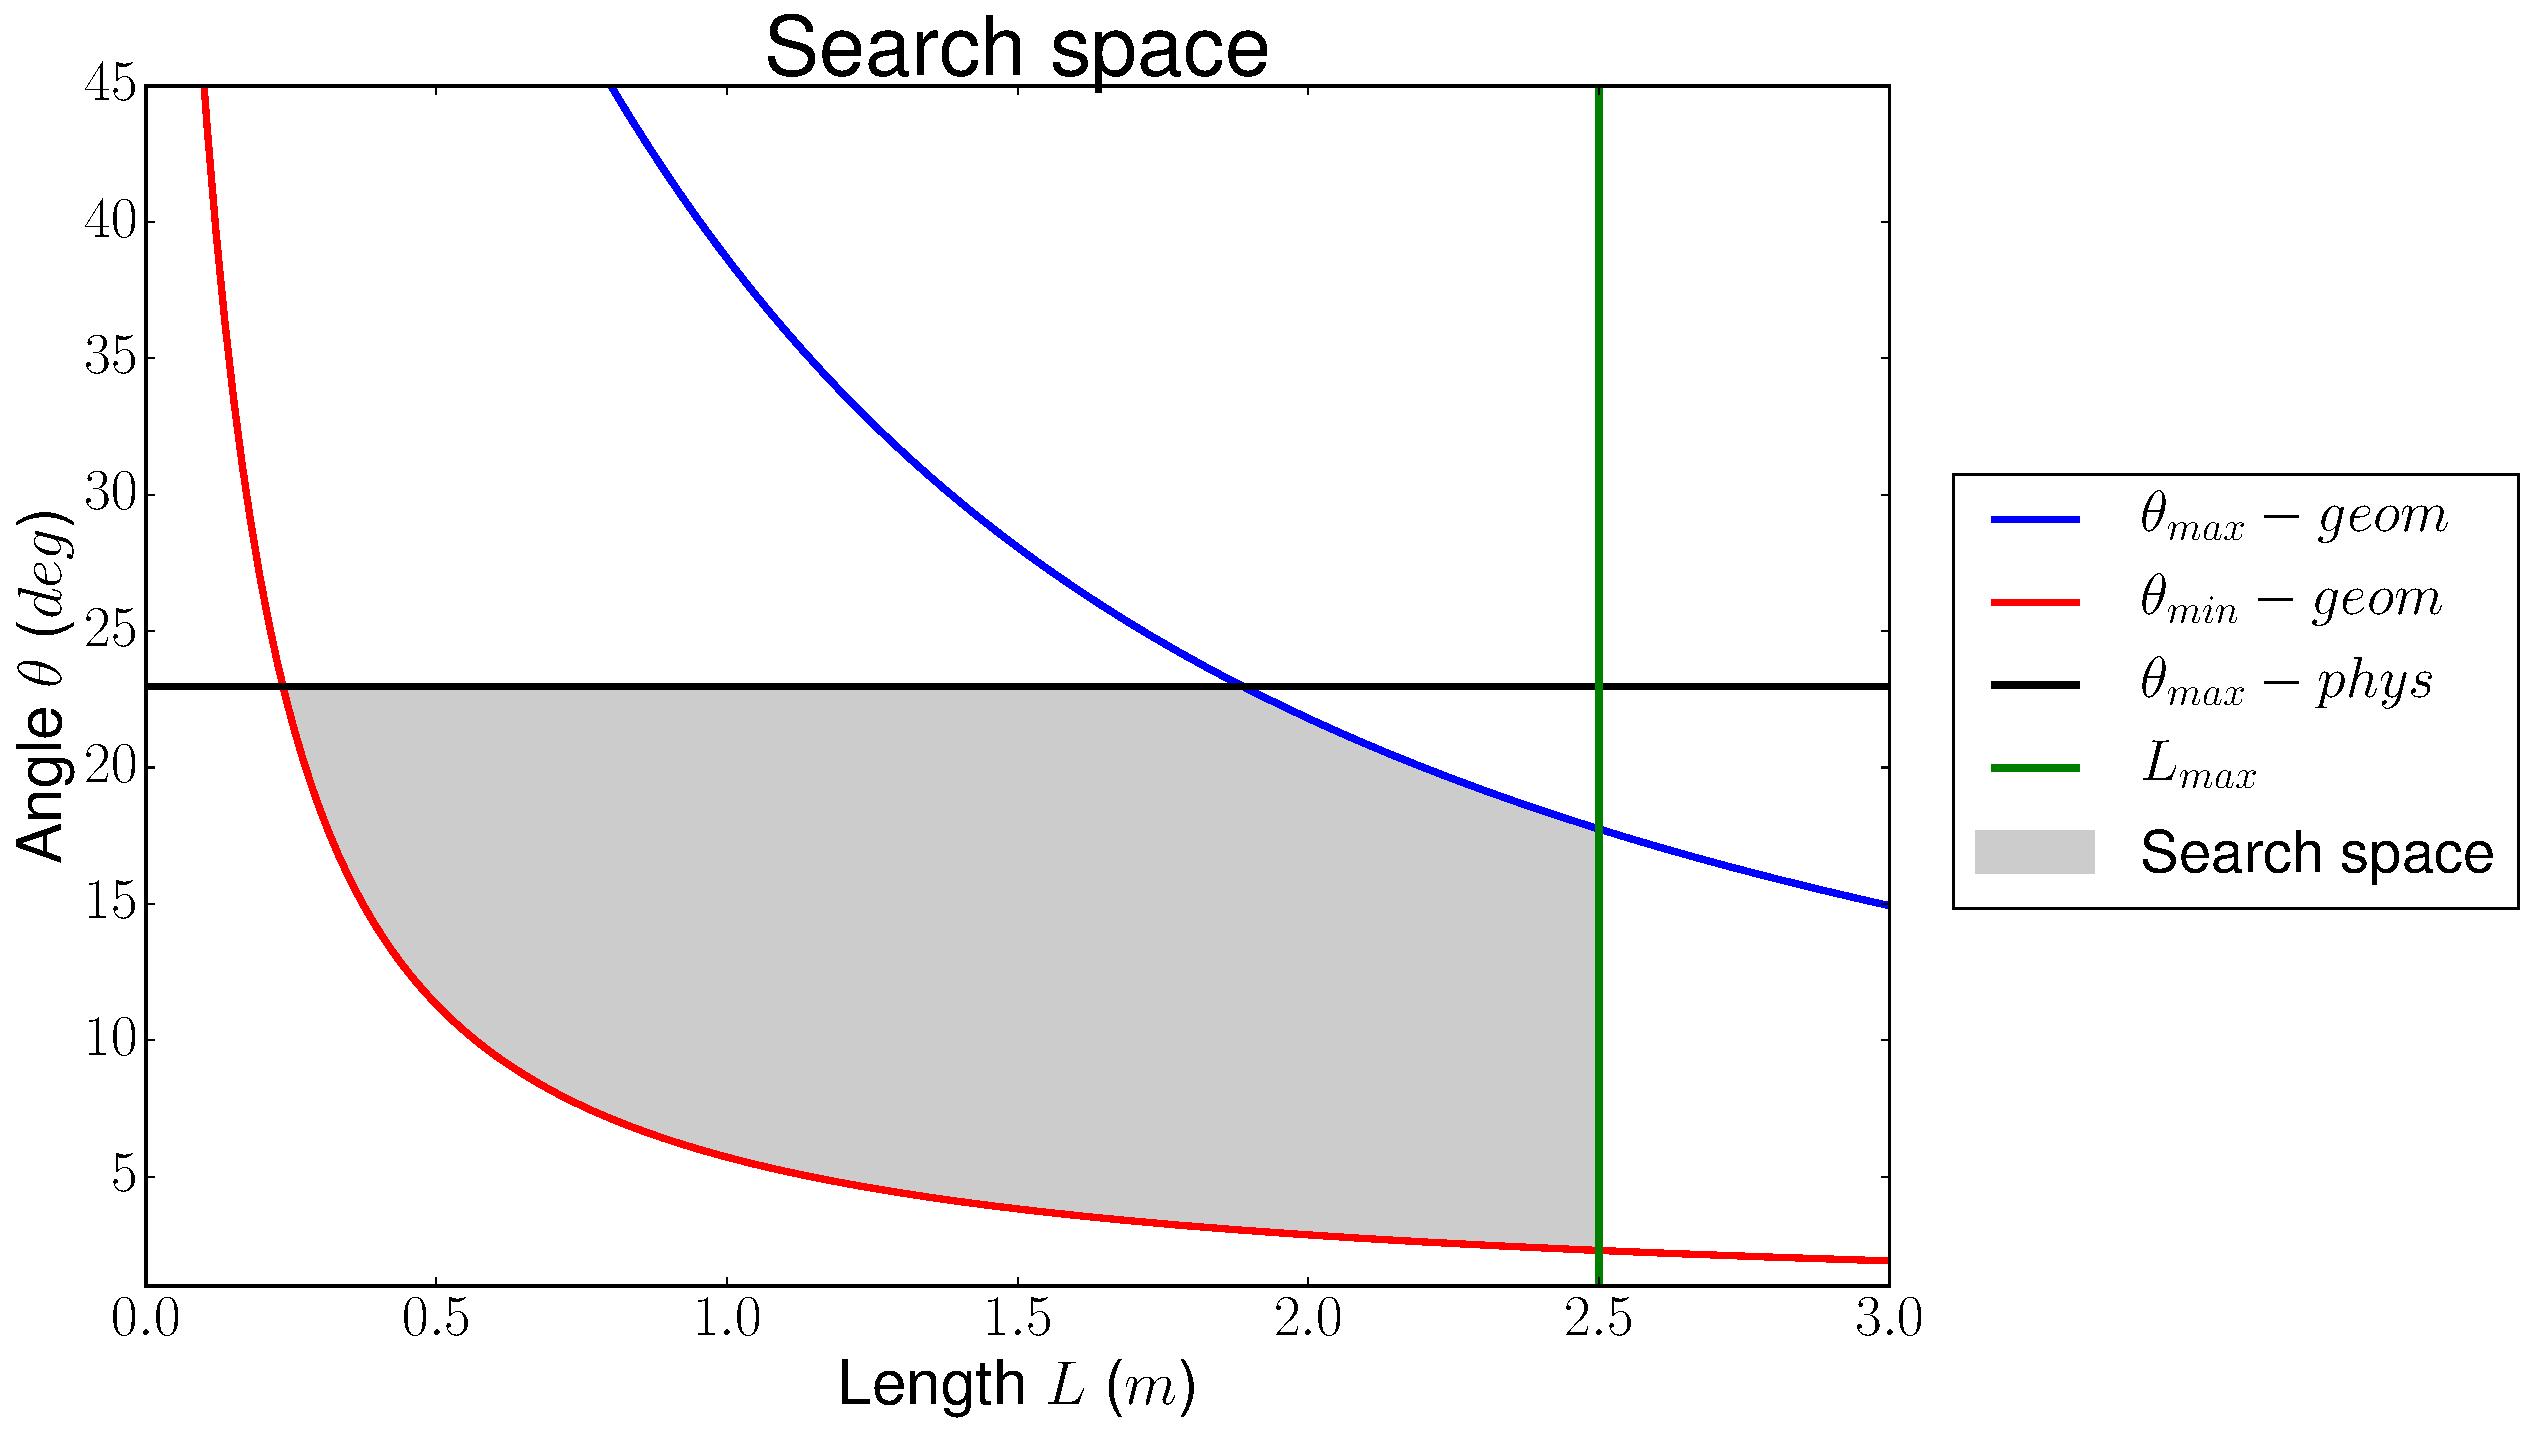
\includegraphics[width=0.85\textwidth]{Figures/3/SearchSpace.pdf}
        \caption{Search space for the diffuser analysis}
        \label{fig:searchSpace}
    \end{figure}

\newpage

The same procedure to determine the best combination of processors as the one followed in the cylinder was done for this case. Here, the optimum number of processors was 16, using a decomposition in 16 subdomains for each one of the cases. Mesh convergence was also performed, taking as most optimum values the ones obtained from a high-resolution mesh simulated with the same conditions as the case here presented. One consideration when selecting the mesh size was the time for performing each simulation, given that the simulation of one generation of 32 individuals took 2 hours, without including the fitness evaluation. 

The mesh is composed of 8 blocks with the sizes described in Figure \ref{fig:diffuserMesh}. The boundary conditions are shown in Figure \ref{fig:diffuserBC} and the type and value for each one of the variables is collected in Table \ref{table:BCdiffuser}. 

    \vspace{10mm}    
    
     \begin{figure}[h!]
        \centering
        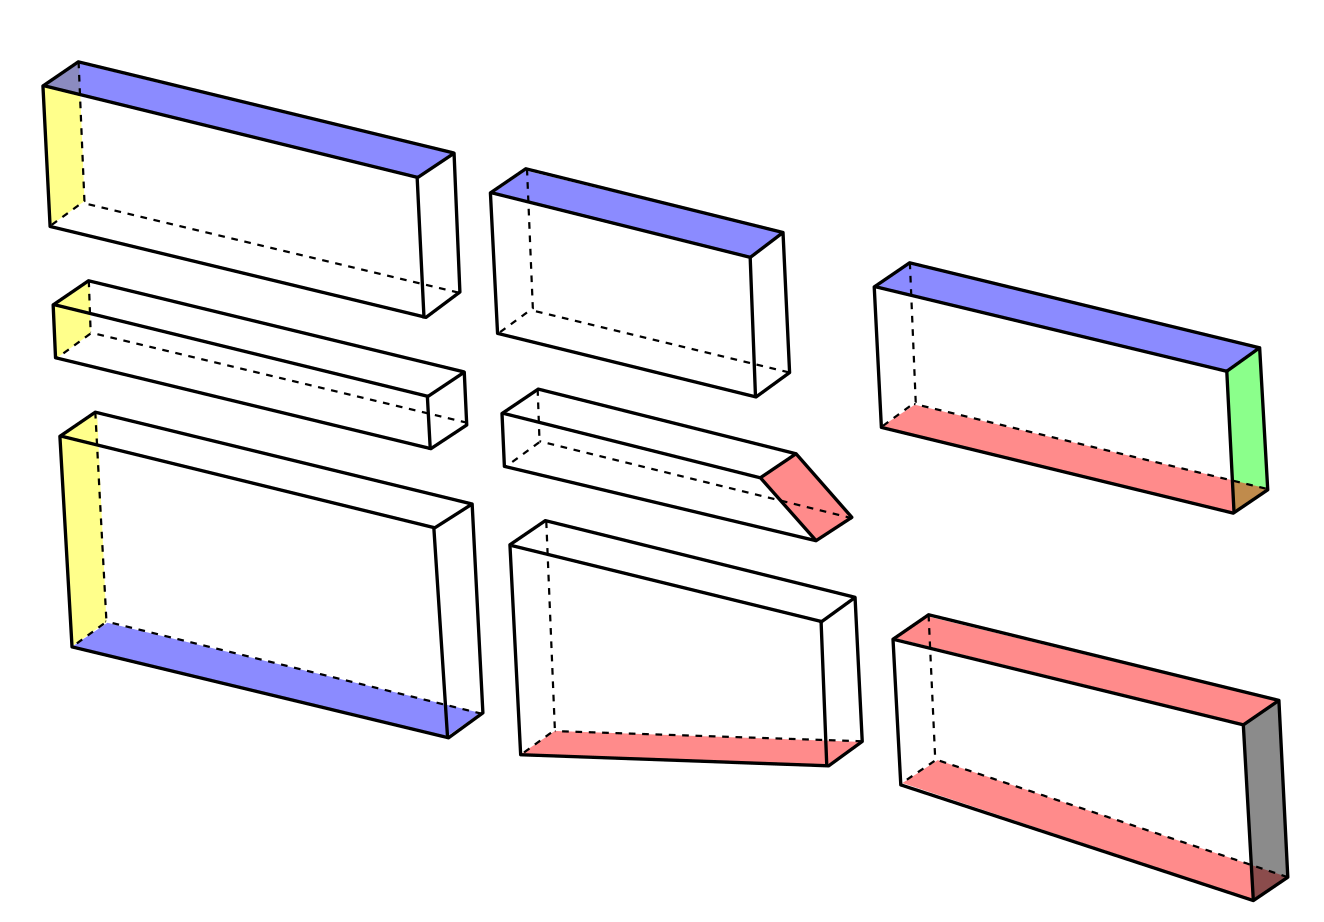
\includegraphics[width=\textwidth]{Figures/3/diffuserBC.png}
        \caption{Exploded view of the mesh for the diffuser case}
        \label{fig:diffuserBC}
    \end{figure}
    
    
\newpage
    
            \begin{table}[h!]
        \centering
           \footnotesize
        \caption{Boundary conditions for the diffuser case}
        \label{table:BCdiffuser}

        \begin{tabular}{cc}
        \multicolumn{2}{c}{\textbf{Inlet (yellow)}}          \\
        \hline
        $U$                    & \texttt{fixedValue (590 0 0)}           \\
        $p$                     &  \texttt{fixedValue 19930}          \\
        $T$                     &  \texttt{fixedValue 216}          \\
        $k$                    & \texttt{turbulentIntensityKineticEnergyInlet 2}  \\
        $\epsilon$                    &      \texttt{turbulentMixingLengthDissipationRateInlet 200} \\
        $\nu_t$                    & \texttt{calculated 0.00001}           \\
        $\alpha_t$                    & \texttt{calculated 0.01}           \\
        & \\
        \multicolumn{2}{c}{\textbf{Outlet (green)}}          \\
        \hline
        $U$                   & \texttt{zeroGradient}           \\
        $p$                     &  \texttt{zeroGradient}          \\
        $T$                     &  \texttt{zeroGradient}          \\
        $k$                    & \texttt{inletOutlet 2}           \\
        $\epsilon$                    & \texttt{inletOutlet 200}           \\
        $\nu_t$                    & \texttt{calculated 0.00001}           \\
        $\alpha_t$                    & \texttt{calculated 0.01}           \\
        & \\
        \multicolumn{2}{c}{\textbf{Engine (grey)}}      \\
        \hline
        $U$                    & \texttt{zeroGradient}           \\
        $p$                     &  \texttt{zeroGradient}          \\
        $T$                     &  \texttt{zeroGradient}          \\
        $k$                    & \texttt{inletOutlet 2}           \\
        $\epsilon$                    & \texttt{inletOutlet 200}           \\
        $\nu_t$                    & \texttt{calculated 0.00001}           \\
        $\alpha_t$                    & \texttt{calculated 0.01}           \\
        & \\
        \multicolumn{2}{c}{\textbf{Wall: cowl \& axis (red)}}           \\
        \hline
        $U$                    & \texttt{fixedValue (0 0 0)}           \\
        $p$                     &  \texttt{zeroGradient}          \\
        $T$                     &  \texttt{zeroGradient}          \\
        $k$                    & \texttt{kqRWallFunction 2}           \\
        $\epsilon$                    & \texttt{epsilonWallFunction 200}           \\
        $\nu_t$                    & \texttt{nutkWallFunction 0.0}           \\
        $\alpha_t$                    & \texttt{alphatWallFunction 0.01}           \\
        & \\

        \multicolumn{2}{c}{\textbf{Upper/Lower (blue)}}      \\
        \hline
        $U$                    & \texttt{inletOutlet (590 0 0)}           \\
        $p$                     &  \texttt{zeroGradient}          \\
        $T$                     &  \texttt{zeroGradient}          \\
        $k$                    & \texttt{inletOutlet 2}           \\
        $\epsilon$                    & \texttt{inletOutlet 200}           \\
        $\nu_t$                    & \texttt{calculated 0.00001}           \\
        $\alpha_t$                    & \texttt{calculated 0.01}           \\
                & \\

        \multicolumn{2}{c}{\textbf{Front/Back (white)}}      \\
        \hline
        $\texttt{*}$                    & empty \\
        \end{tabular}
        \end{table}

\vspace{2mm}

\newpage

\subsection{Airfoil design}


The most typical use of optimization algorithms in CFD techniques is the design of airfoils. However, the classical approach is done via adjoint shape methods, achieving the most optimum airfoil by varying the mesh shape. Other approaches try to adjust the different splines that form the airfoil applying then panel methods theory. In this study, the application of genetic algorithms and computer fluid dynamics to achieve the most optimal airfoil will be addressed. 

As said there are a lot of ways of parametrizing one airfoil. There are also families of airfoils described by some number, such as the NACA family. But for a first approach, it will be interesting to begin with a more straightforward parametrization. Joukowsky airfoils are one of those sets that are usually used for potential flow but they may be compared with some NACA airfoils, having that the transformation is more than a mathematical construction \cite{kapania2008modeling}.

Joukowsky transformation is a mathematical operation that takes one circle in the $\zeta$ complex plane and transforms it to an airfoil in the $z$ plane. The position of the circle and its radius will determine the shape of the airfoil, so the way of parametrizing the airfoil will be the $\mu_x$ and $\mu_y$ as the coordinates for the center and the radius $R$. Joukowsky transform is:
\begin{equation}
z=\zeta+\dfrac{1}{\zeta}
\end{equation}
where $z = x + y\ i$ and $\zeta = \chi + \eta\ i$. 

     \begin{figure}[h!]
        \centering
        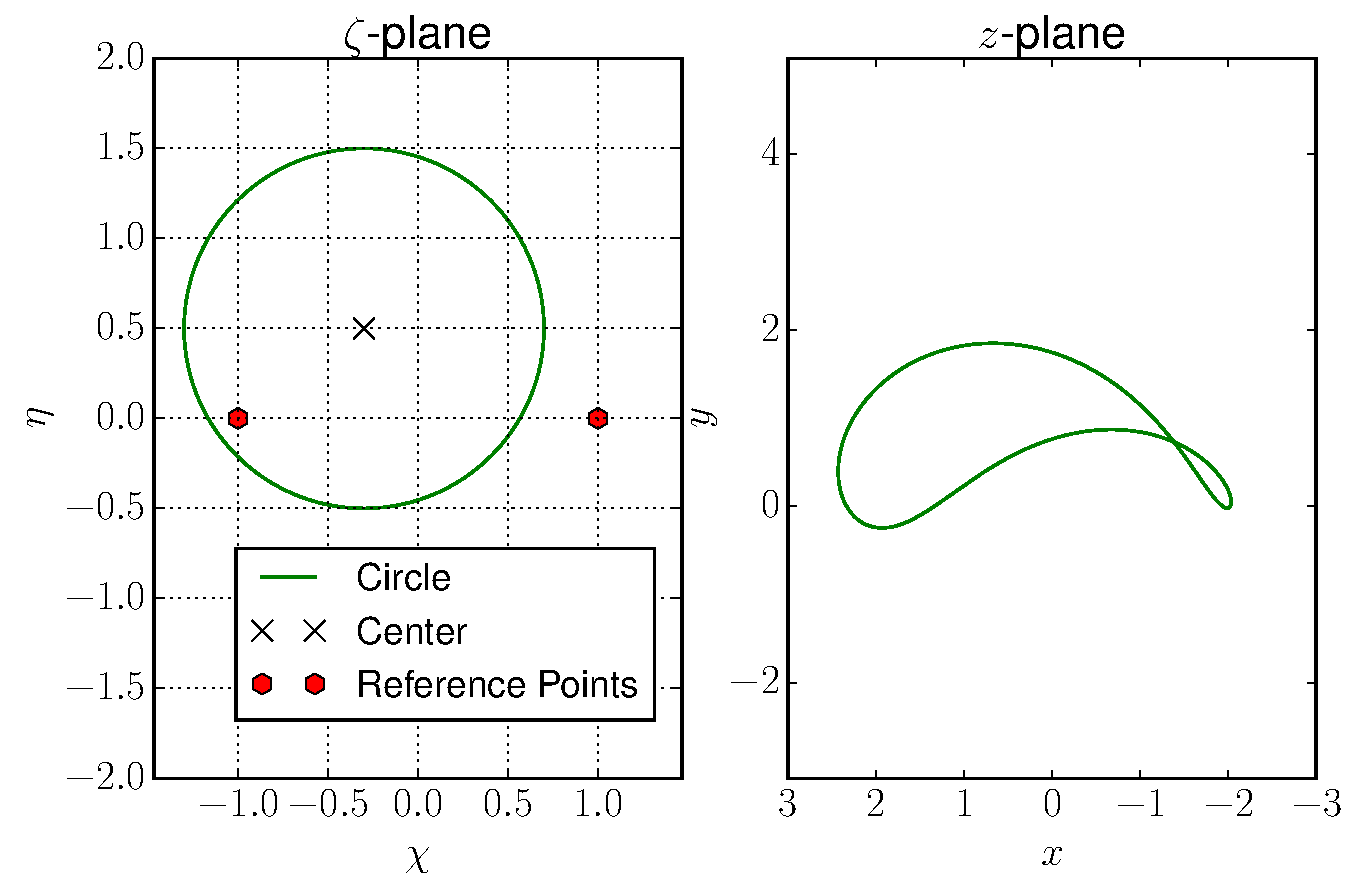
\includegraphics[width=0.8\textwidth]{Figures/3/nonJouk2.pdf}
        \caption{Example of a Joukowsky airfoil with non valid $\mu_x$, $\mu_y$ and $R$}
        \label{fig:nonJoukowsky}
    \end{figure}

\newpage

Taking a closer look to Joukowsky airfoils, they only have realistic shapes if the circle in $\zeta$ intercepts the point $\zeta = (-1,0)$ or the point $\zeta = (1,0)$ (as it can be seen in Figure \ref{fig:nonJoukowsky}). This way the radius will be determined with the position of the center of the circle, having $R=f(\mu_x,\mu_y)$. Thus the search variables that form the parameter space are $\mu_x$ and $\mu_y$, which are the coordinates of the center of the circle in the $\zeta$ plane in the $\chi$ and $\eta$.

     \begin{figure}[h!]
        \centering
        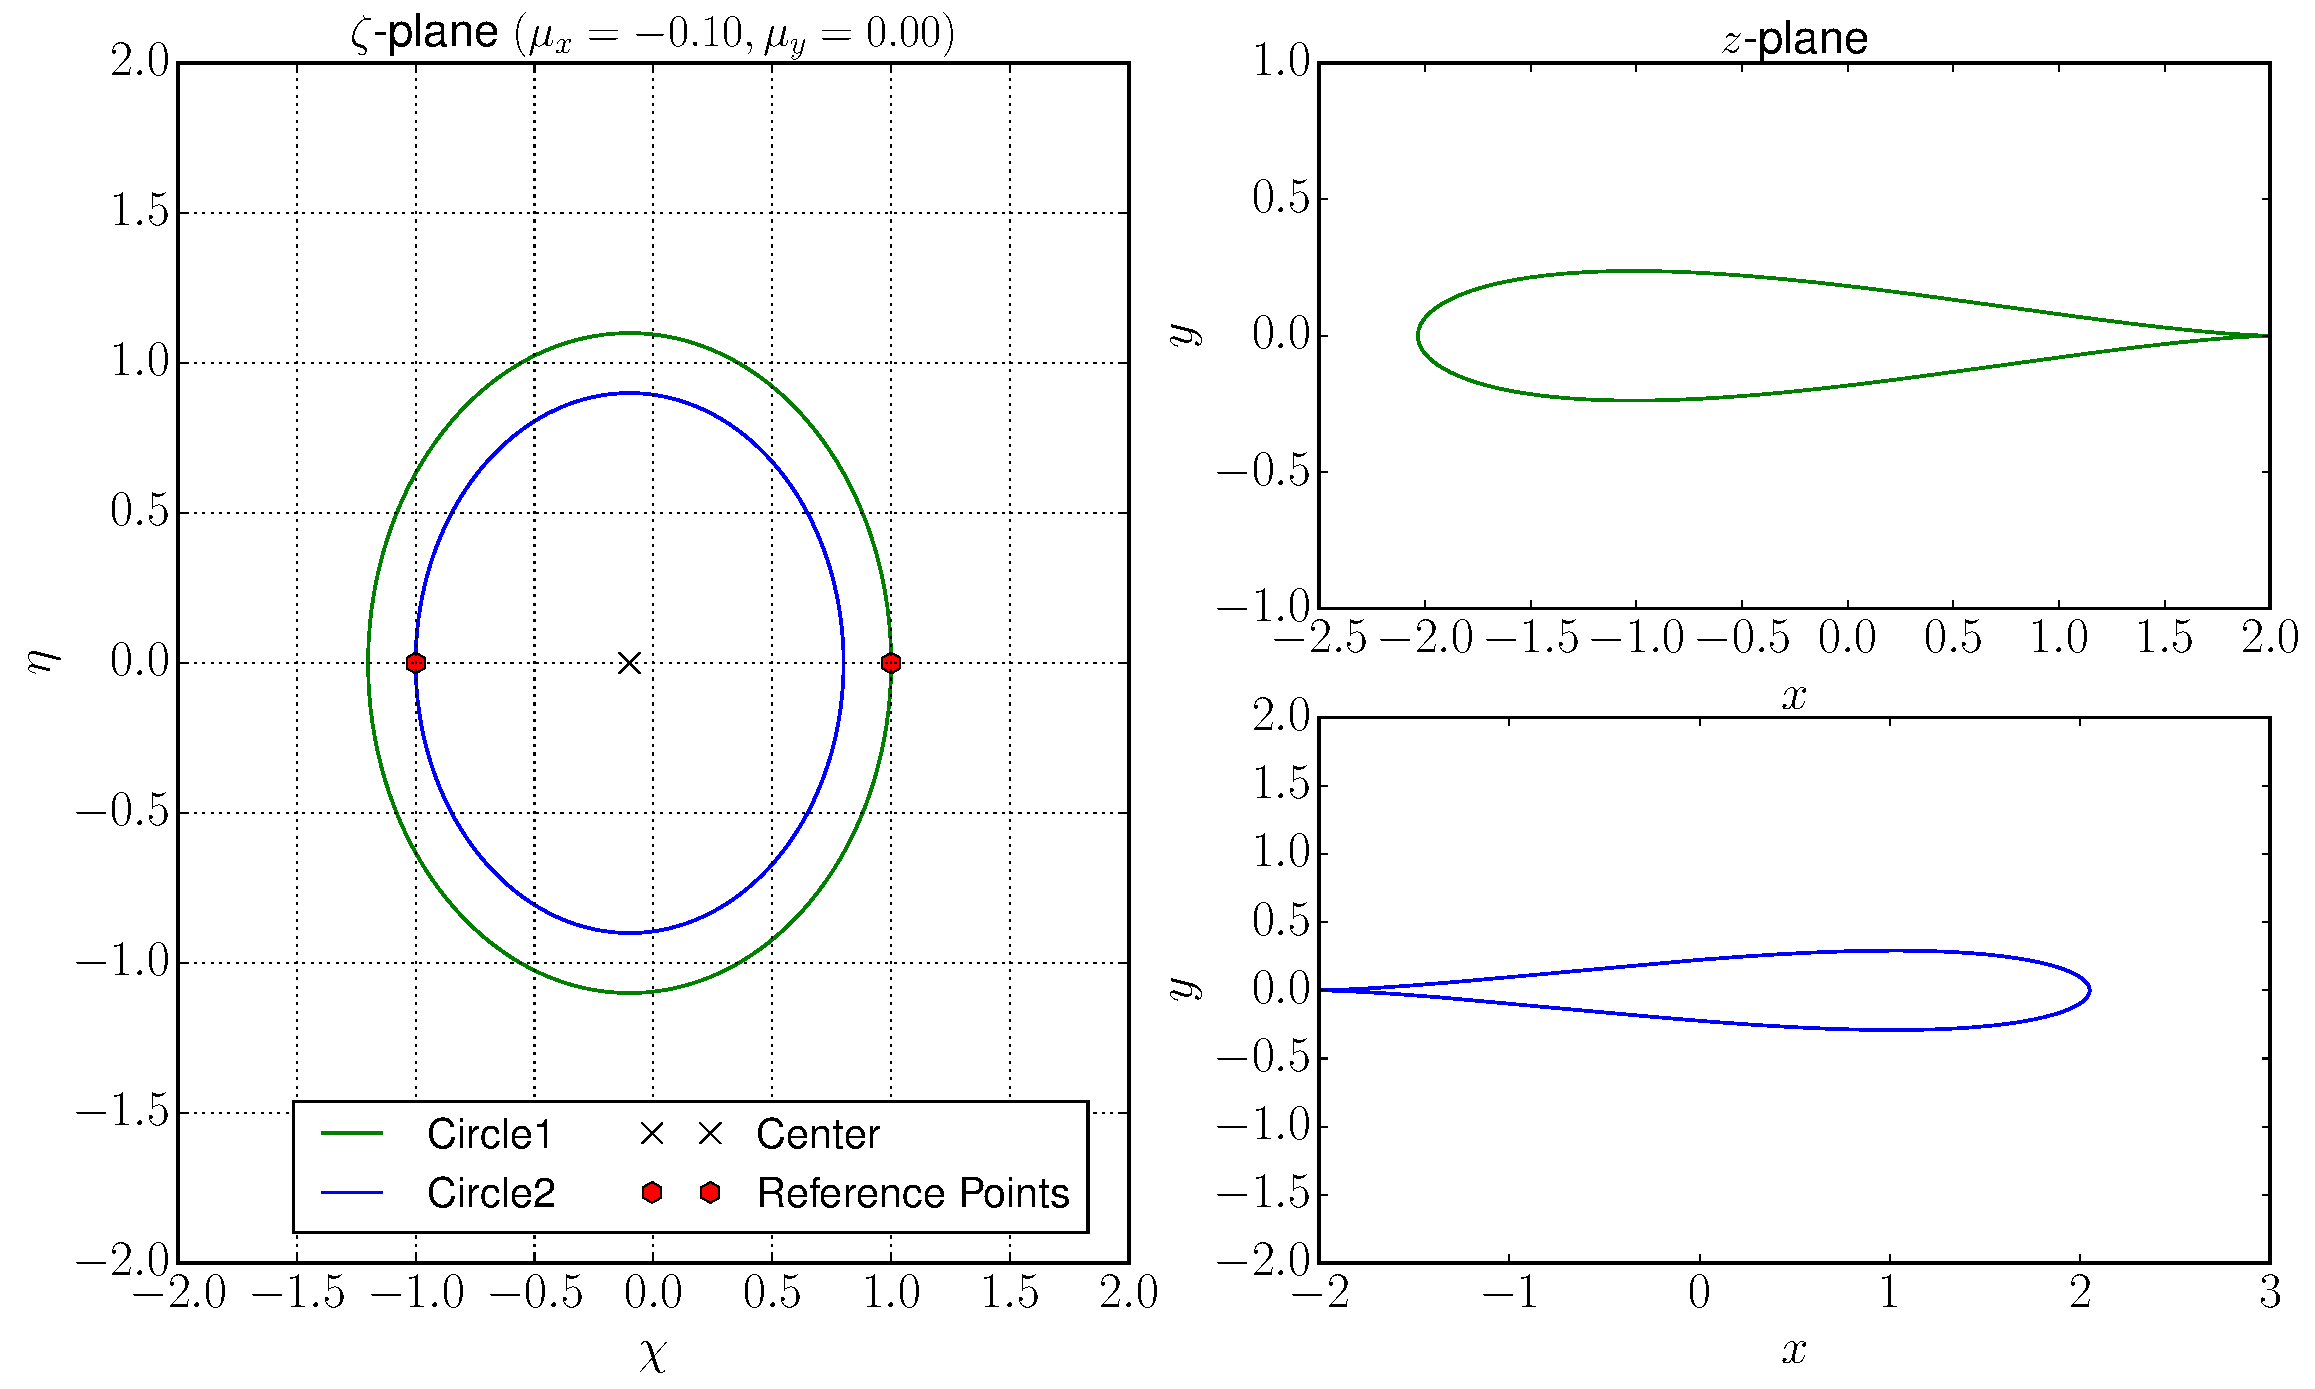
\includegraphics[width=\textwidth]{Figures/3/J_0.pdf}
        \caption{Example of a Joukowsky airfoil defined just with $\mu_x$ and $\mu_y$}
        \label{fig:joukowskyTheory}
    \end{figure}
    
Two simulations were carried out, selecting different objectives to define the function space. These objectives can be easily changed by simply varying the \texttt{fitness.py} script, where the objectives are selected and saved to create the next generation:

\begin{itemize}
    \item Maximization of lift and minimization of drag: these are the most common objectives when trying to optimize an airfoil. Nevertheless, it is impossible to get the optimum value of both at the same time.
    \item Maximization of lift-to-drag ratio and maximization of the airfoil area: this kind of objectives also try to maximize lift and minimize drag (mixed in the $L/D$ ratio) while keeping the inner area of the airfoil as bigger as possible (provided that airfoils carry the fuel in the wings it will be interesting to maximize it). 
\end{itemize}

\newpage

\subsubsection*{Case setup}

In this case, the individuals will have the search space variables represented in the mesh. The shape of the airfoil will depend on the value of $\mu_x$ and $\mu_y$, which are the search variables. The search space will be bounded inside the range $\mu_x\in[-0.3,-0.1]$ and $\mu_y\in[0.0,0.15]$. The simulation was performed with an incompressible solver in a steady-state fashion (\texttt{simpleFoam}) for at least 2500 iterations. The turbulence was modeled with the Spalart-Allmaras RAS model and a Newtonian flow was assumed. The density was chosen at sea level ($\rho=1.225\ kg\cdot m^{-3}$) as well as the viscosity value of $\nu=1.789\times10^{-5}\ m^2\cdot s^{-1}$. The airfoil faced a free stream velocity of $30\ m\cdot s^{-1}$ with turbulence values as selected for a similar OpenFOAM tutorial case ($\tilde{\nu}=0.14$ and $\nu_t =0.14$). This corresponds to a Reynolds number of $Re=2.05\times10^6$.

The mesh geometry consisted of a rectangle with a circular inlet that encased the airfoil. Joukowsky airfoils may have a wide range of possible chords, but for this analysis, the chord has been normalized to a value of one. The other dimensions of the mesh are chosen with respect to the normalized chord value and choosing them far enough so boundary conditions do not affect the flow and close enough so the computational domain is not too big. The refinement of the boundary layer was done in a very generic way, provided that the airfoil may acquire a great variety of shapes. However, and taking advantage of the fact that the mesh was done with hexahedral blocks, some boundary layer inflation was done (with simple expansion ratio gradings). 


     \begin{figure}[h!]
        \centering
        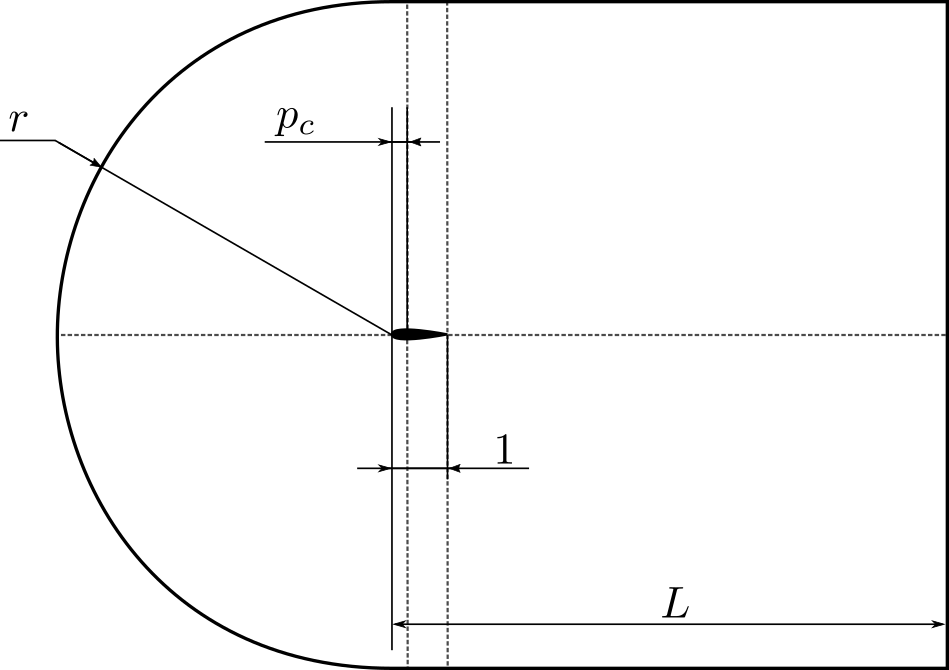
\includegraphics[width=0.7\textwidth]{Figures/3/airfoil2dReport.png}
        \caption{Mesh schematics of the airfoil}
        \label{fig:airofilMesh}
    \end{figure}

    
    
     \begin{figure}[h!]
        \centering
        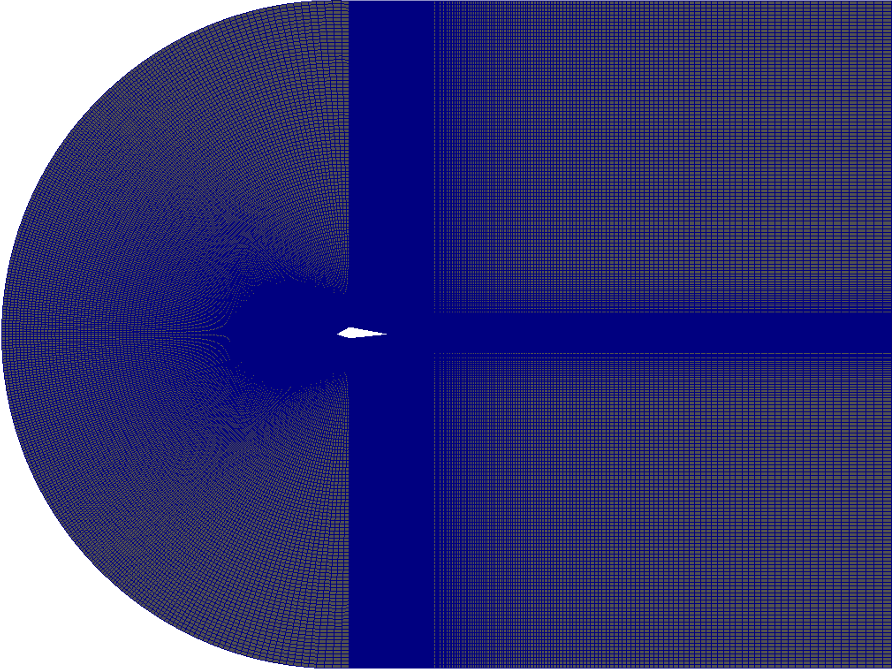
\includegraphics[width=0.7\textwidth]{Figures/3/joukOverview.png}
        \caption{Mesh for the airfoil optimization case}
        \label{fig:airofilMeshPF}
    \end{figure}

The process of creating the airfoil was automatically done with Python, but the progress of introducing the points of the spline that represents the airfoil is shown in Figures \ref{fig:uncomputedJoukowsky} and \ref{fig:computedJoukowsky}, where the airfoil is delimited by the hexahedral blocks, converting it to arcs that represent the value of $\mu_x$ and $\mu_y$.

     \begin{figure}[h!]
        \centering
        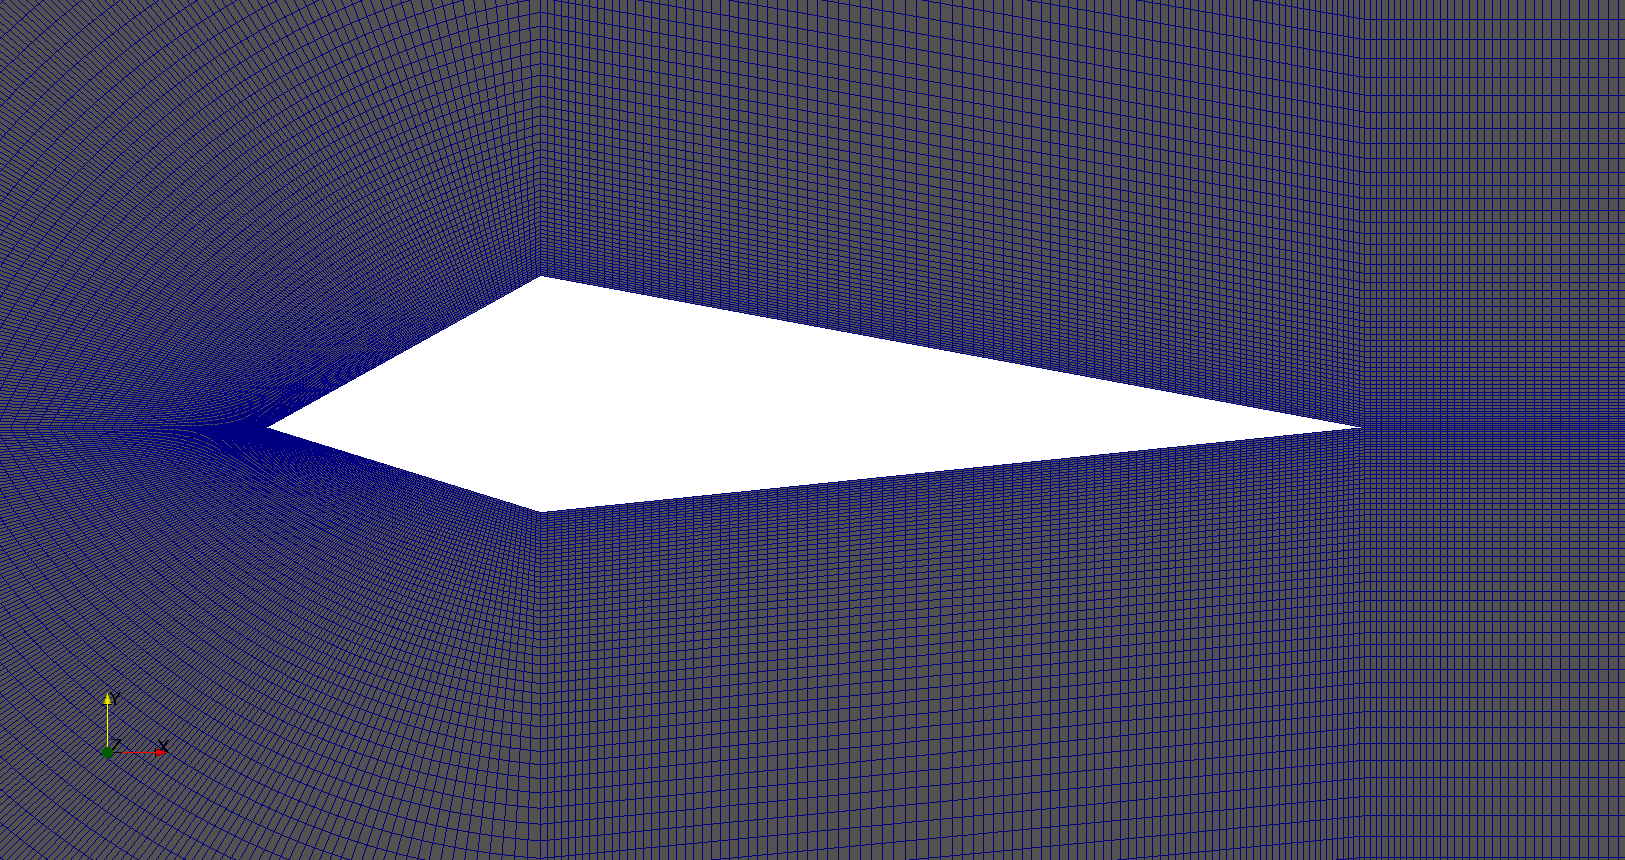
\includegraphics[width=\textwidth]{Figures/3/joukRombo.png}
        \caption{Mesh picture with the uncomputed airfoil}
        \label{fig:uncomputedJoukowsky}
    \end{figure}

    \newpage
    
     \begin{figure}[h!]
        \centering
        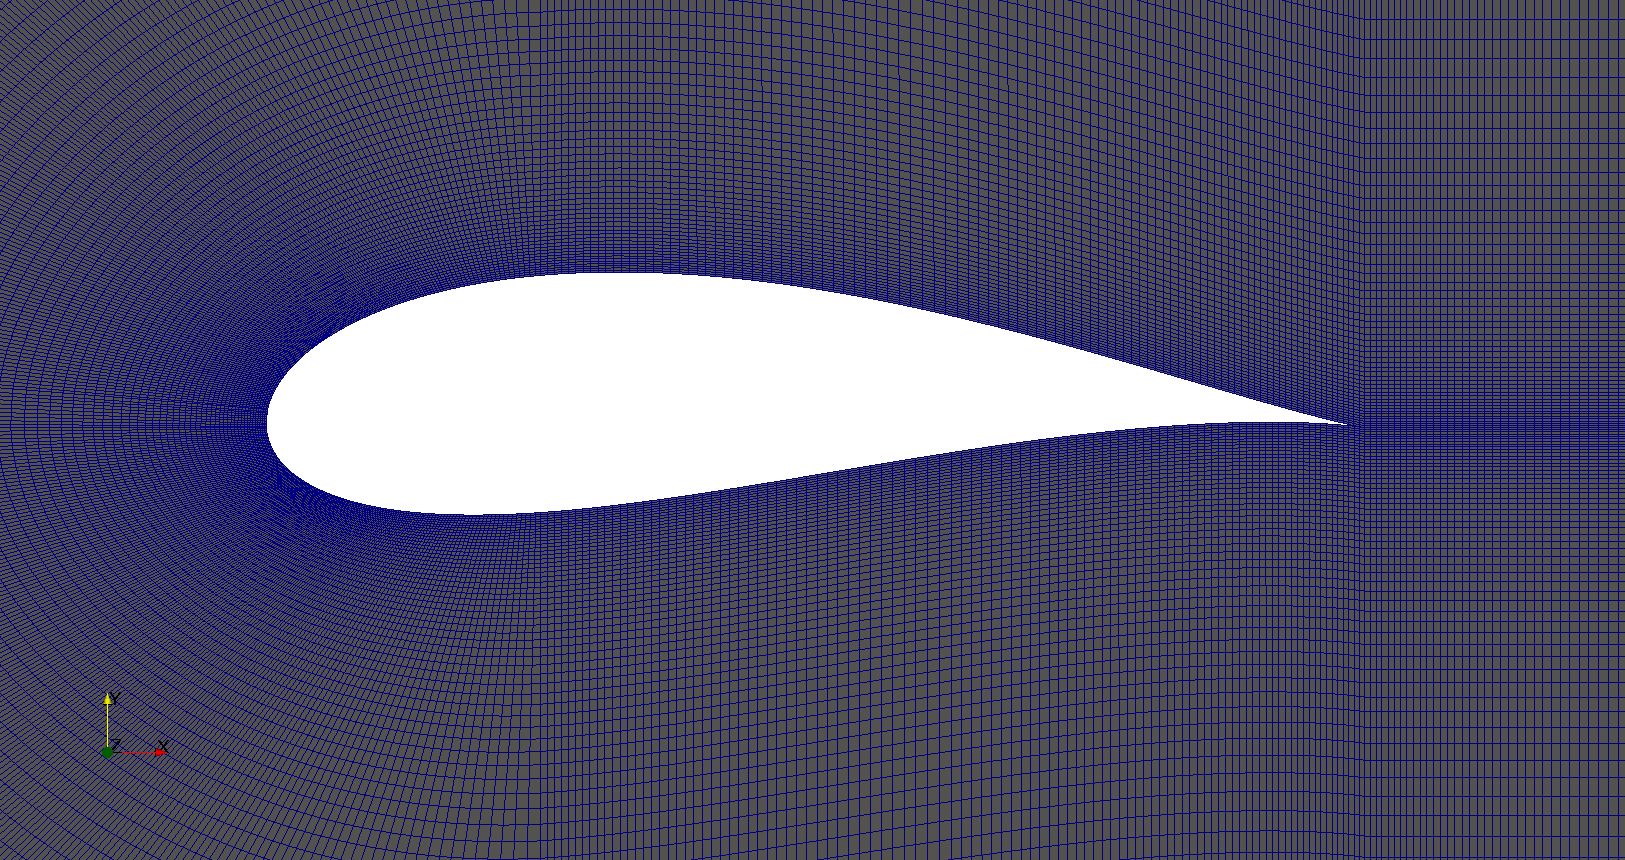
\includegraphics[width=\textwidth]{Figures/3/joukFoil.png}
        \caption{Computed airfoil in the mesh}
        \label{fig:computedJoukowsky}
    \end{figure}
        
    The boundary conditions used for the two optimization setups were the same. A freestream enters the domain through the yellow face and leaves it through the green one. Given that the angle of attack $\alpha$ is zero, there is no need of any special refinements or critical considerations about mass conservation in the domain (whereas doing angle of attack simulations will require a refined mesh and take into account the possible problems that upper and lower boundary conditions may have). 

    \vspace{3mm}    
    
     \begin{figure}[h!]
        \centering
        \small
        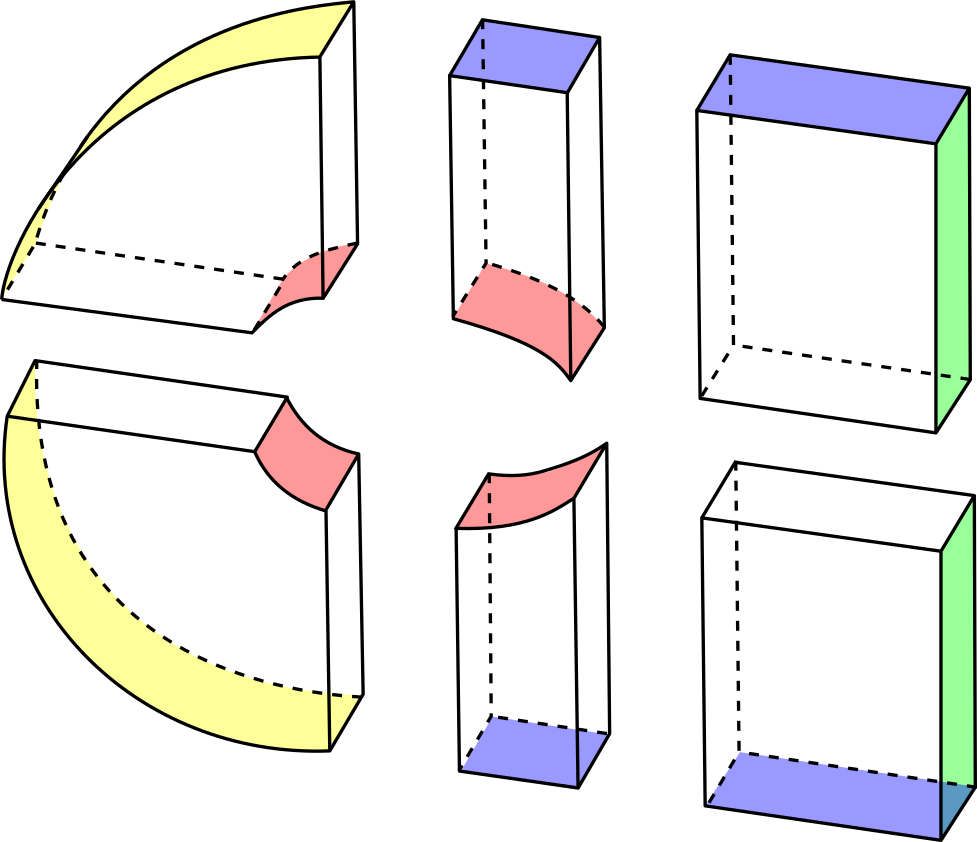
\includegraphics[width=0.5\textwidth]{Figures/3/airfoilBC.png}
        \caption{Airfoil exploded view of the mesh with the boundary conditions}
        \label{fig:airofilBCpic}
    \end{figure}
    
    \newpage
    
    The boundary conditions are listed in Table \ref{table:airfoilBC}:
   
        \begin{table}[h!]
        \centering
        \small
        \caption{Boundary conditions for the airfoil cases}
        \label{table:airfoilBC}
        \begin{tabular}{cc}
        \multicolumn{2}{c}{\textbf{Inlet (yellow)}}          \\
        \hline
        $U$                    & \texttt{freestream (30 0 0)}           \\
        $p$                     &  \texttt{freestreamPressure}          \\
        $\tilde{\nu}$                    & \texttt{freestream 0.14}           \\
        $\nu_t$                    & \texttt{freestream 0.14}           \\
                & \\

        \multicolumn{2}{c}{\textbf{Outlet (green)}}          \\
        \hline
        $U$                   & \texttt{freestream (30 0 0)}           \\
        $p$                     &  \texttt{freestreamPressure}          \\
        $\tilde{\nu}$                    & \texttt{freestream 0.14}           \\
        $\nu_t$                    & \texttt{freestream 0.14}           \\
        & \\

        \multicolumn{2}{c}{\textbf{Airfoil (red)}}           \\
        \hline
        $U$                    & \texttt{noSlip}           \\
        $p$                     &  \texttt{zeroGradient}          \\
        $\tilde{\nu}$                    & \texttt{fixedValue 0.0}           \\
        $\nu_t$                    & \texttt{nutUSpaldingWallFunction 0.0}           \\
        & \\

        \multicolumn{2}{c}{\textbf{Upper/Lower (blue)}}      \\
        \hline
        $U$                    & \texttt{freestream (30 0 0)}           \\
        $p$                     &  \texttt{freestreamPressure}          \\
        $\tilde{\nu}$                    & \texttt{freestream 0.14}           \\
        $\nu_t$                    & \texttt{freestream 0.14}           \\
                & \\
        \multicolumn{2}{c}{\textbf{Front/Back (white)}}      \\
        \hline
        $\texttt{*}$                    & empty \\
        \end{tabular}
        \end{table}
\chapter{Results}

In this chapter, the results of the four optimizations explained in the previous methodology discussion will be presented. Thus, this chapter will be divided into different sections for each case. First, both the search space and the function space will be presented, showing where the individuals are as generations advance. Given that populations are too large to show all individuals, a sample from the population will be chosen in order to show the convergence of the process to a set of non-dominated solutions. Just the results will be shown, the correspondent discussion will be done in the following sections.

\newpage

\subsubsection*{Supression of cylinder vortex oscillations}

     \begin{figure}[h!]
        \centering
        \small
        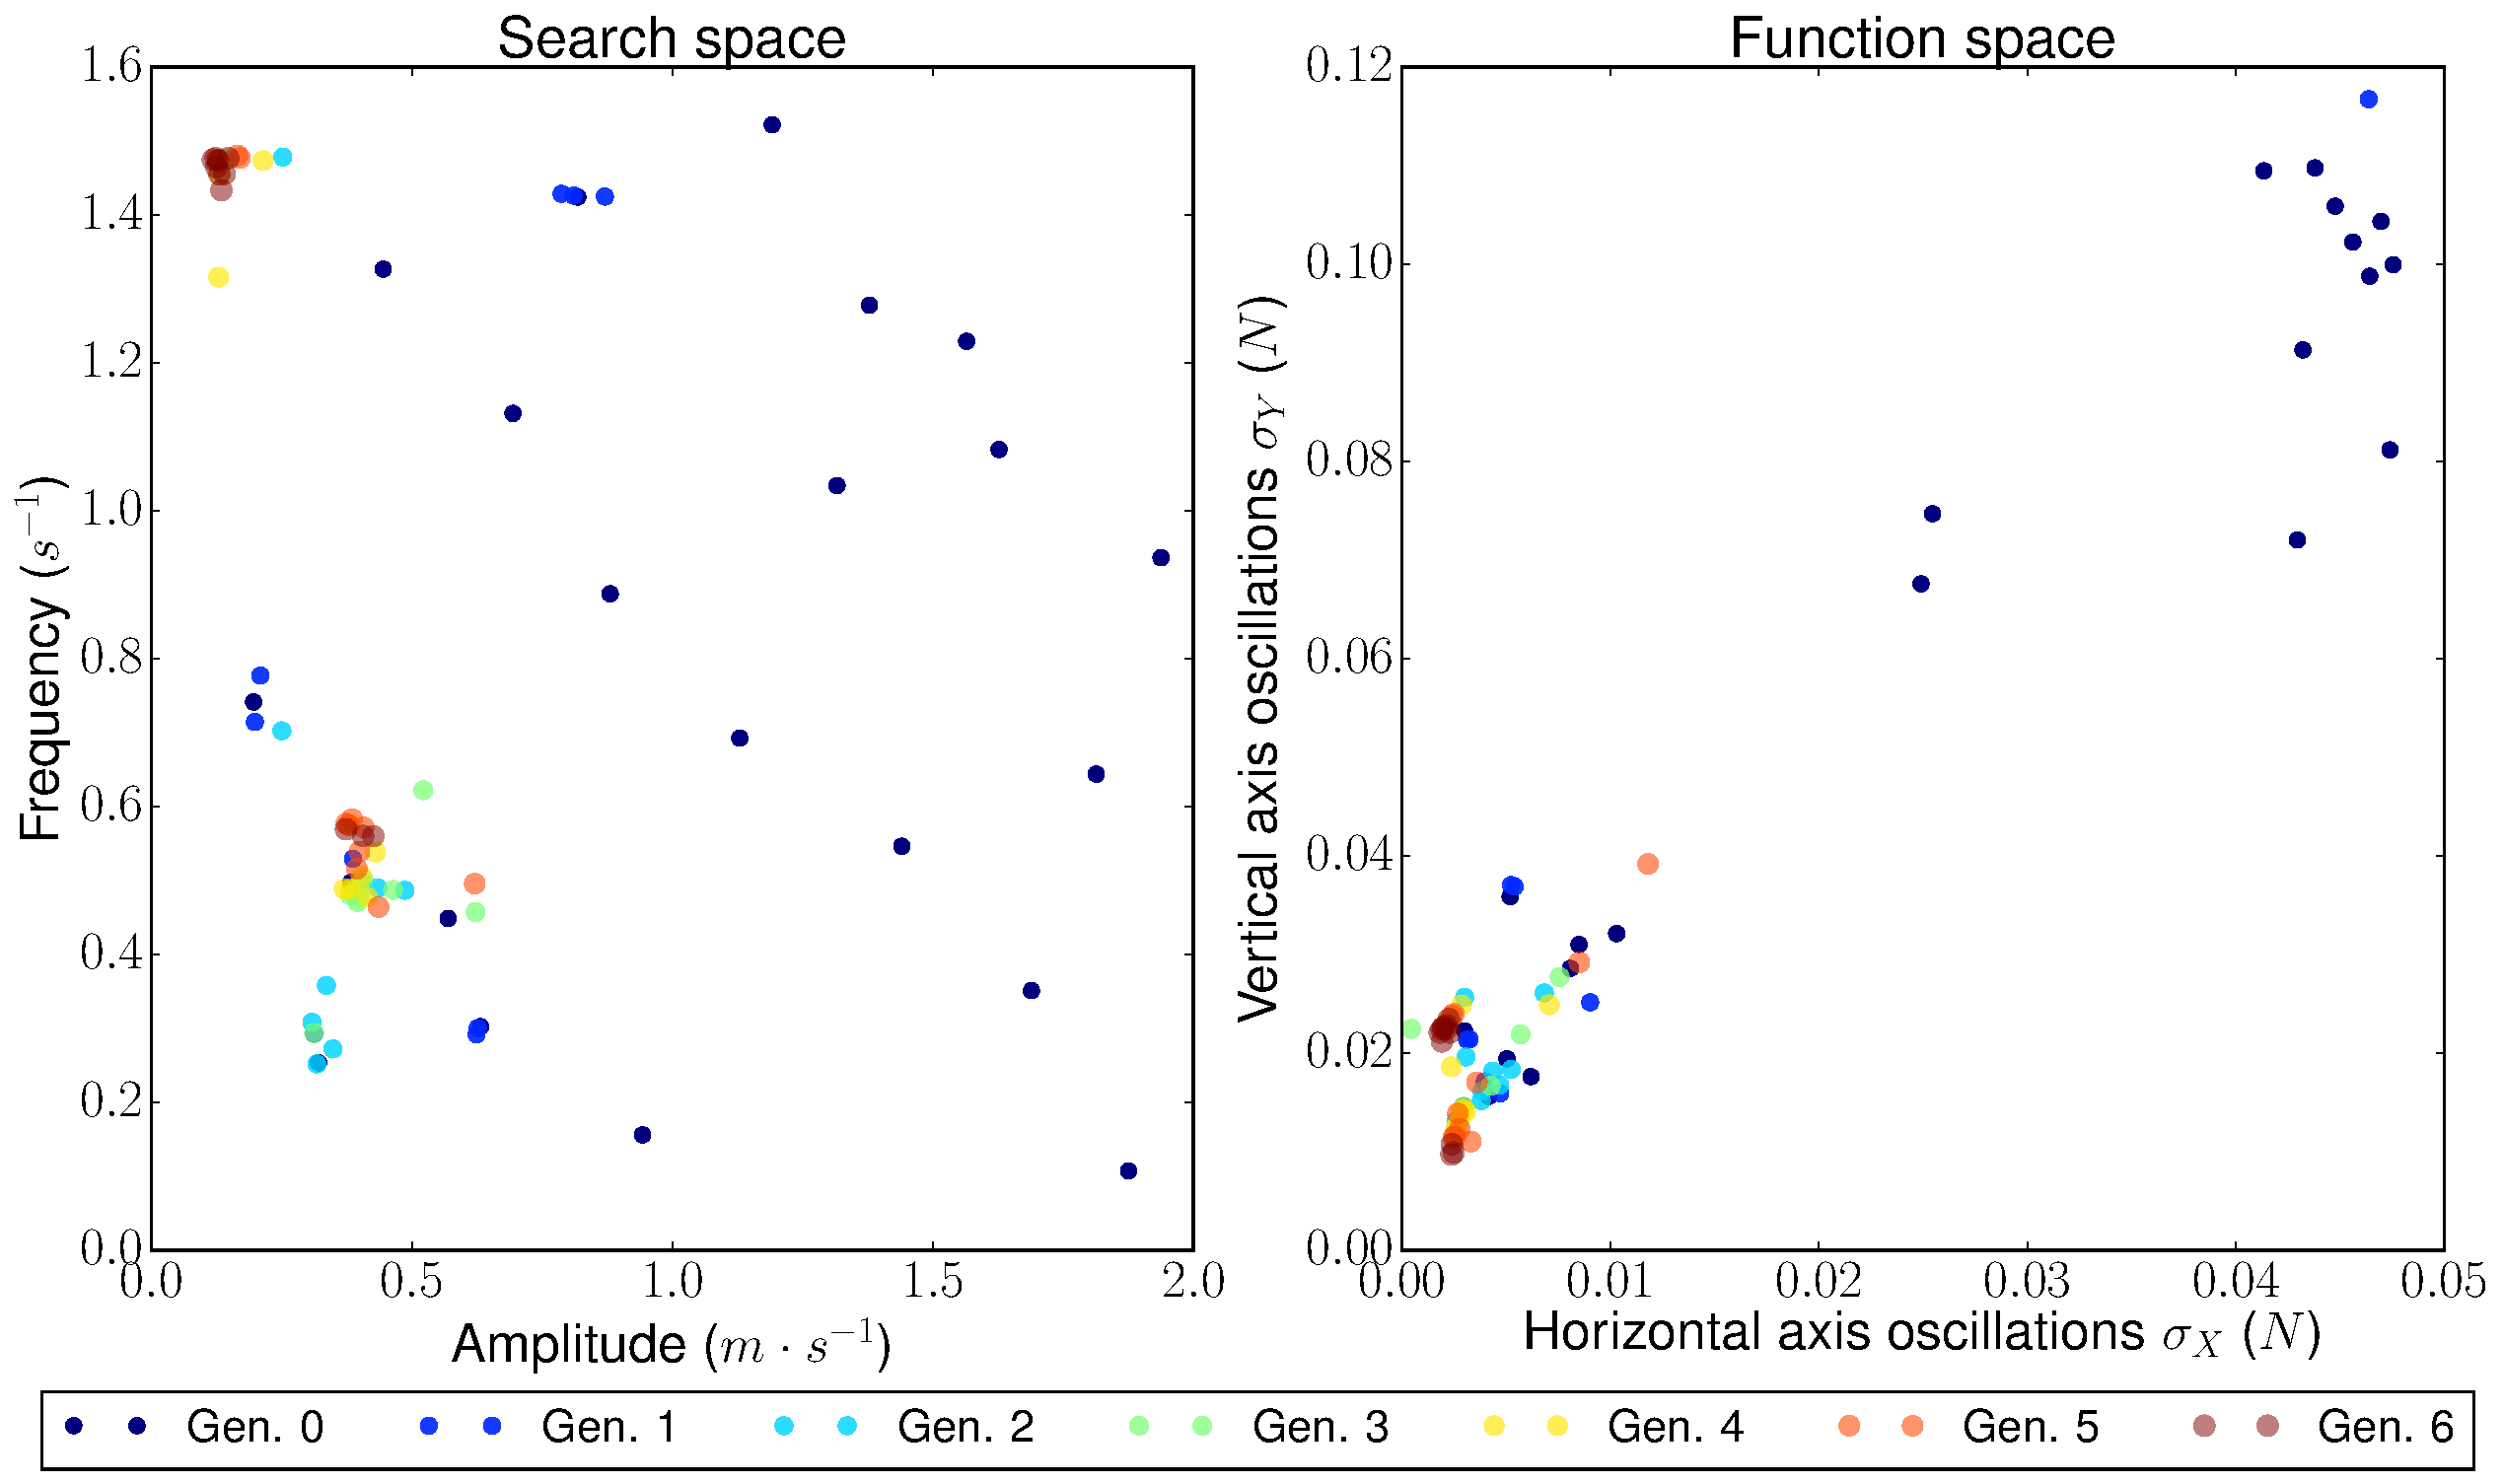
\includegraphics[width=\textwidth, height=0.35\textheight]{Figures/4/gen6.pdf}
        \caption{Evolution of the generations for the cylinder case}
        \label{fig:genForCylinder}
    \end{figure}
    
\begin{figure}[h!]
    \centering
    \begin{subfigure}[t]{0.31\textwidth}
        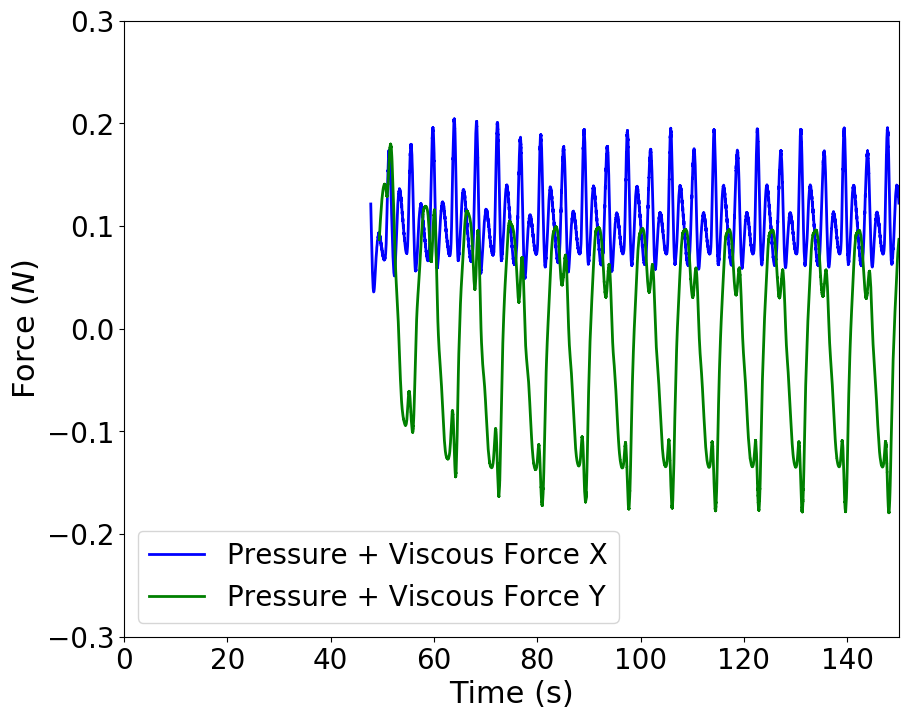
\includegraphics[width=0.95\textwidth, height=0.18\textheight]{Figures/4/OSCg0i37.png}
    \end{subfigure}
    \begin{subfigure}[t]{0.31\textwidth}
        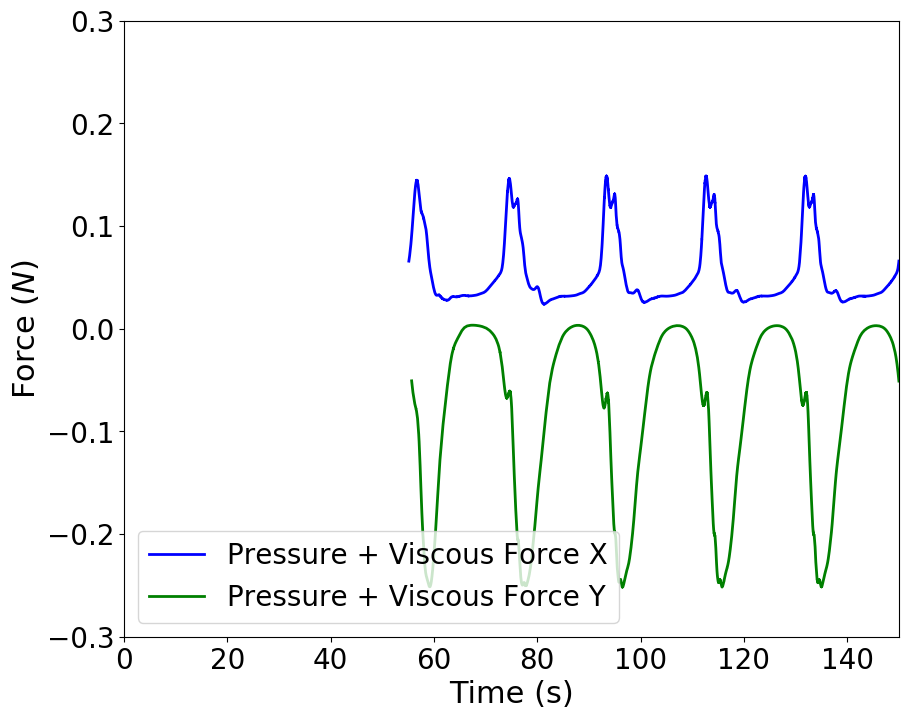
\includegraphics[width=0.95\textwidth, height=0.18\textheight]{Figures/4/OSCg0i38.png}
    \end{subfigure}
    \begin{subfigure}[t]{0.31\textwidth}
        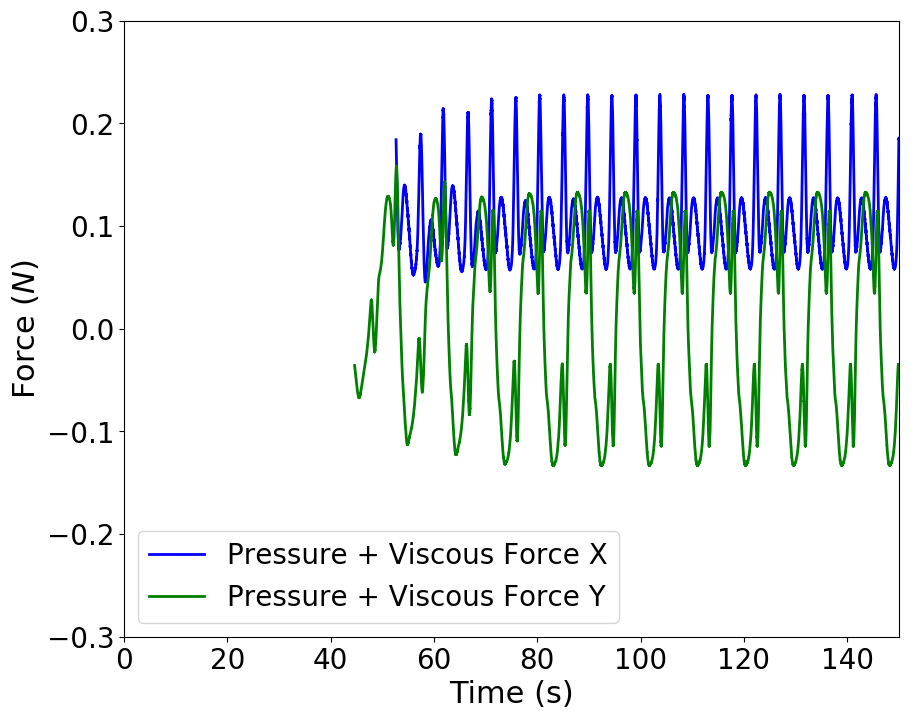
\includegraphics[width=0.95\textwidth, height=0.18\textheight]{Figures/4/OSCg0i45.png}
    \end{subfigure}
    \caption{Sample of the initial generation for the cylinder case}
    \label{fig:initialCyl}
\end{figure}

\begin{figure}[h!]
    \centering
%    \begin{subfigure}[t]{0.15\textwidth}
%    \end{subfigure}
    \begin{subfigure}[t]{0.31\textwidth}
        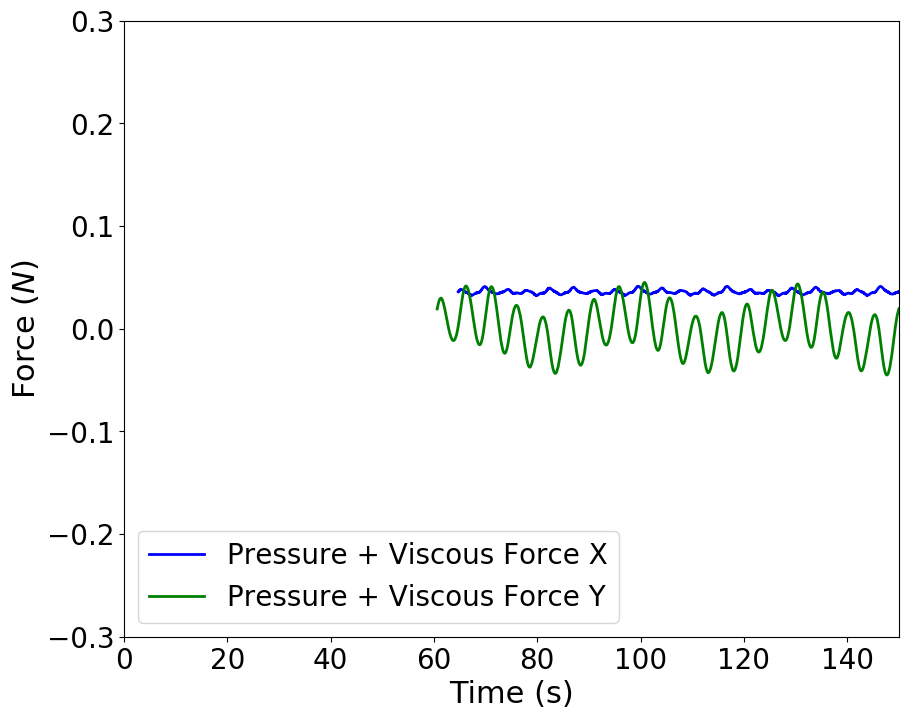
\includegraphics[width=0.95\textwidth, height=0.18\textheight]{Figures/4/OSCg6i6.png}
    \end{subfigure}
    \begin{subfigure}[t]{0.31\textwidth}
        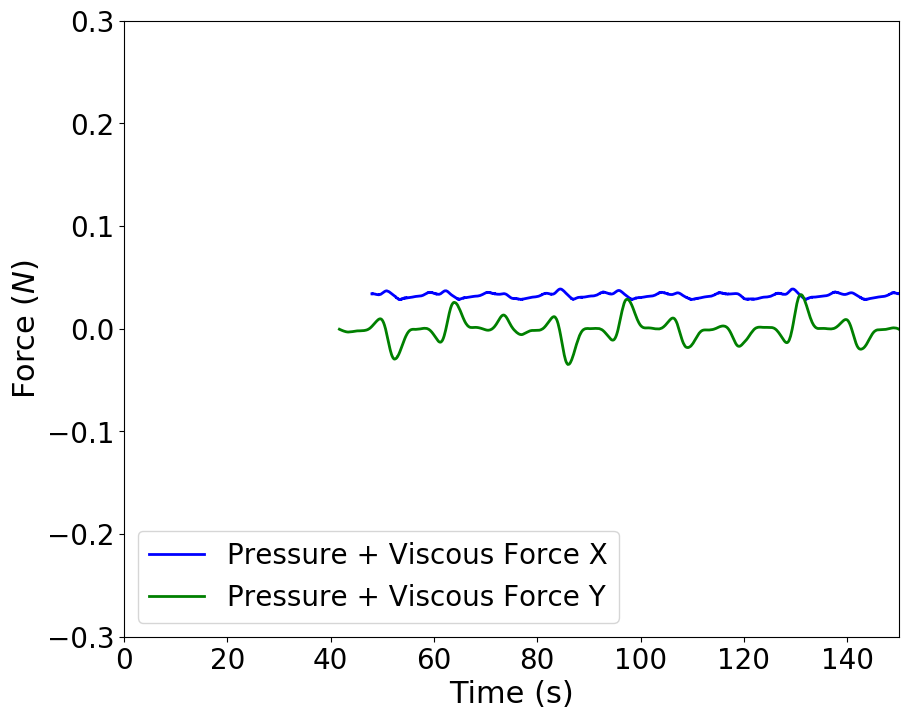
\includegraphics[width=0.95\textwidth, height=0.18\textheight]{Figures/4/OSCg6i3.png}
    \end{subfigure}
    \caption{Sample of the final generation for the cylinder case}
    \label{fig:finalCyl}
\end{figure}

\newpage

\subsubsection*{Inlet of diffuser geometry}

     \begin{figure}[h!]
        \centering
        \small
        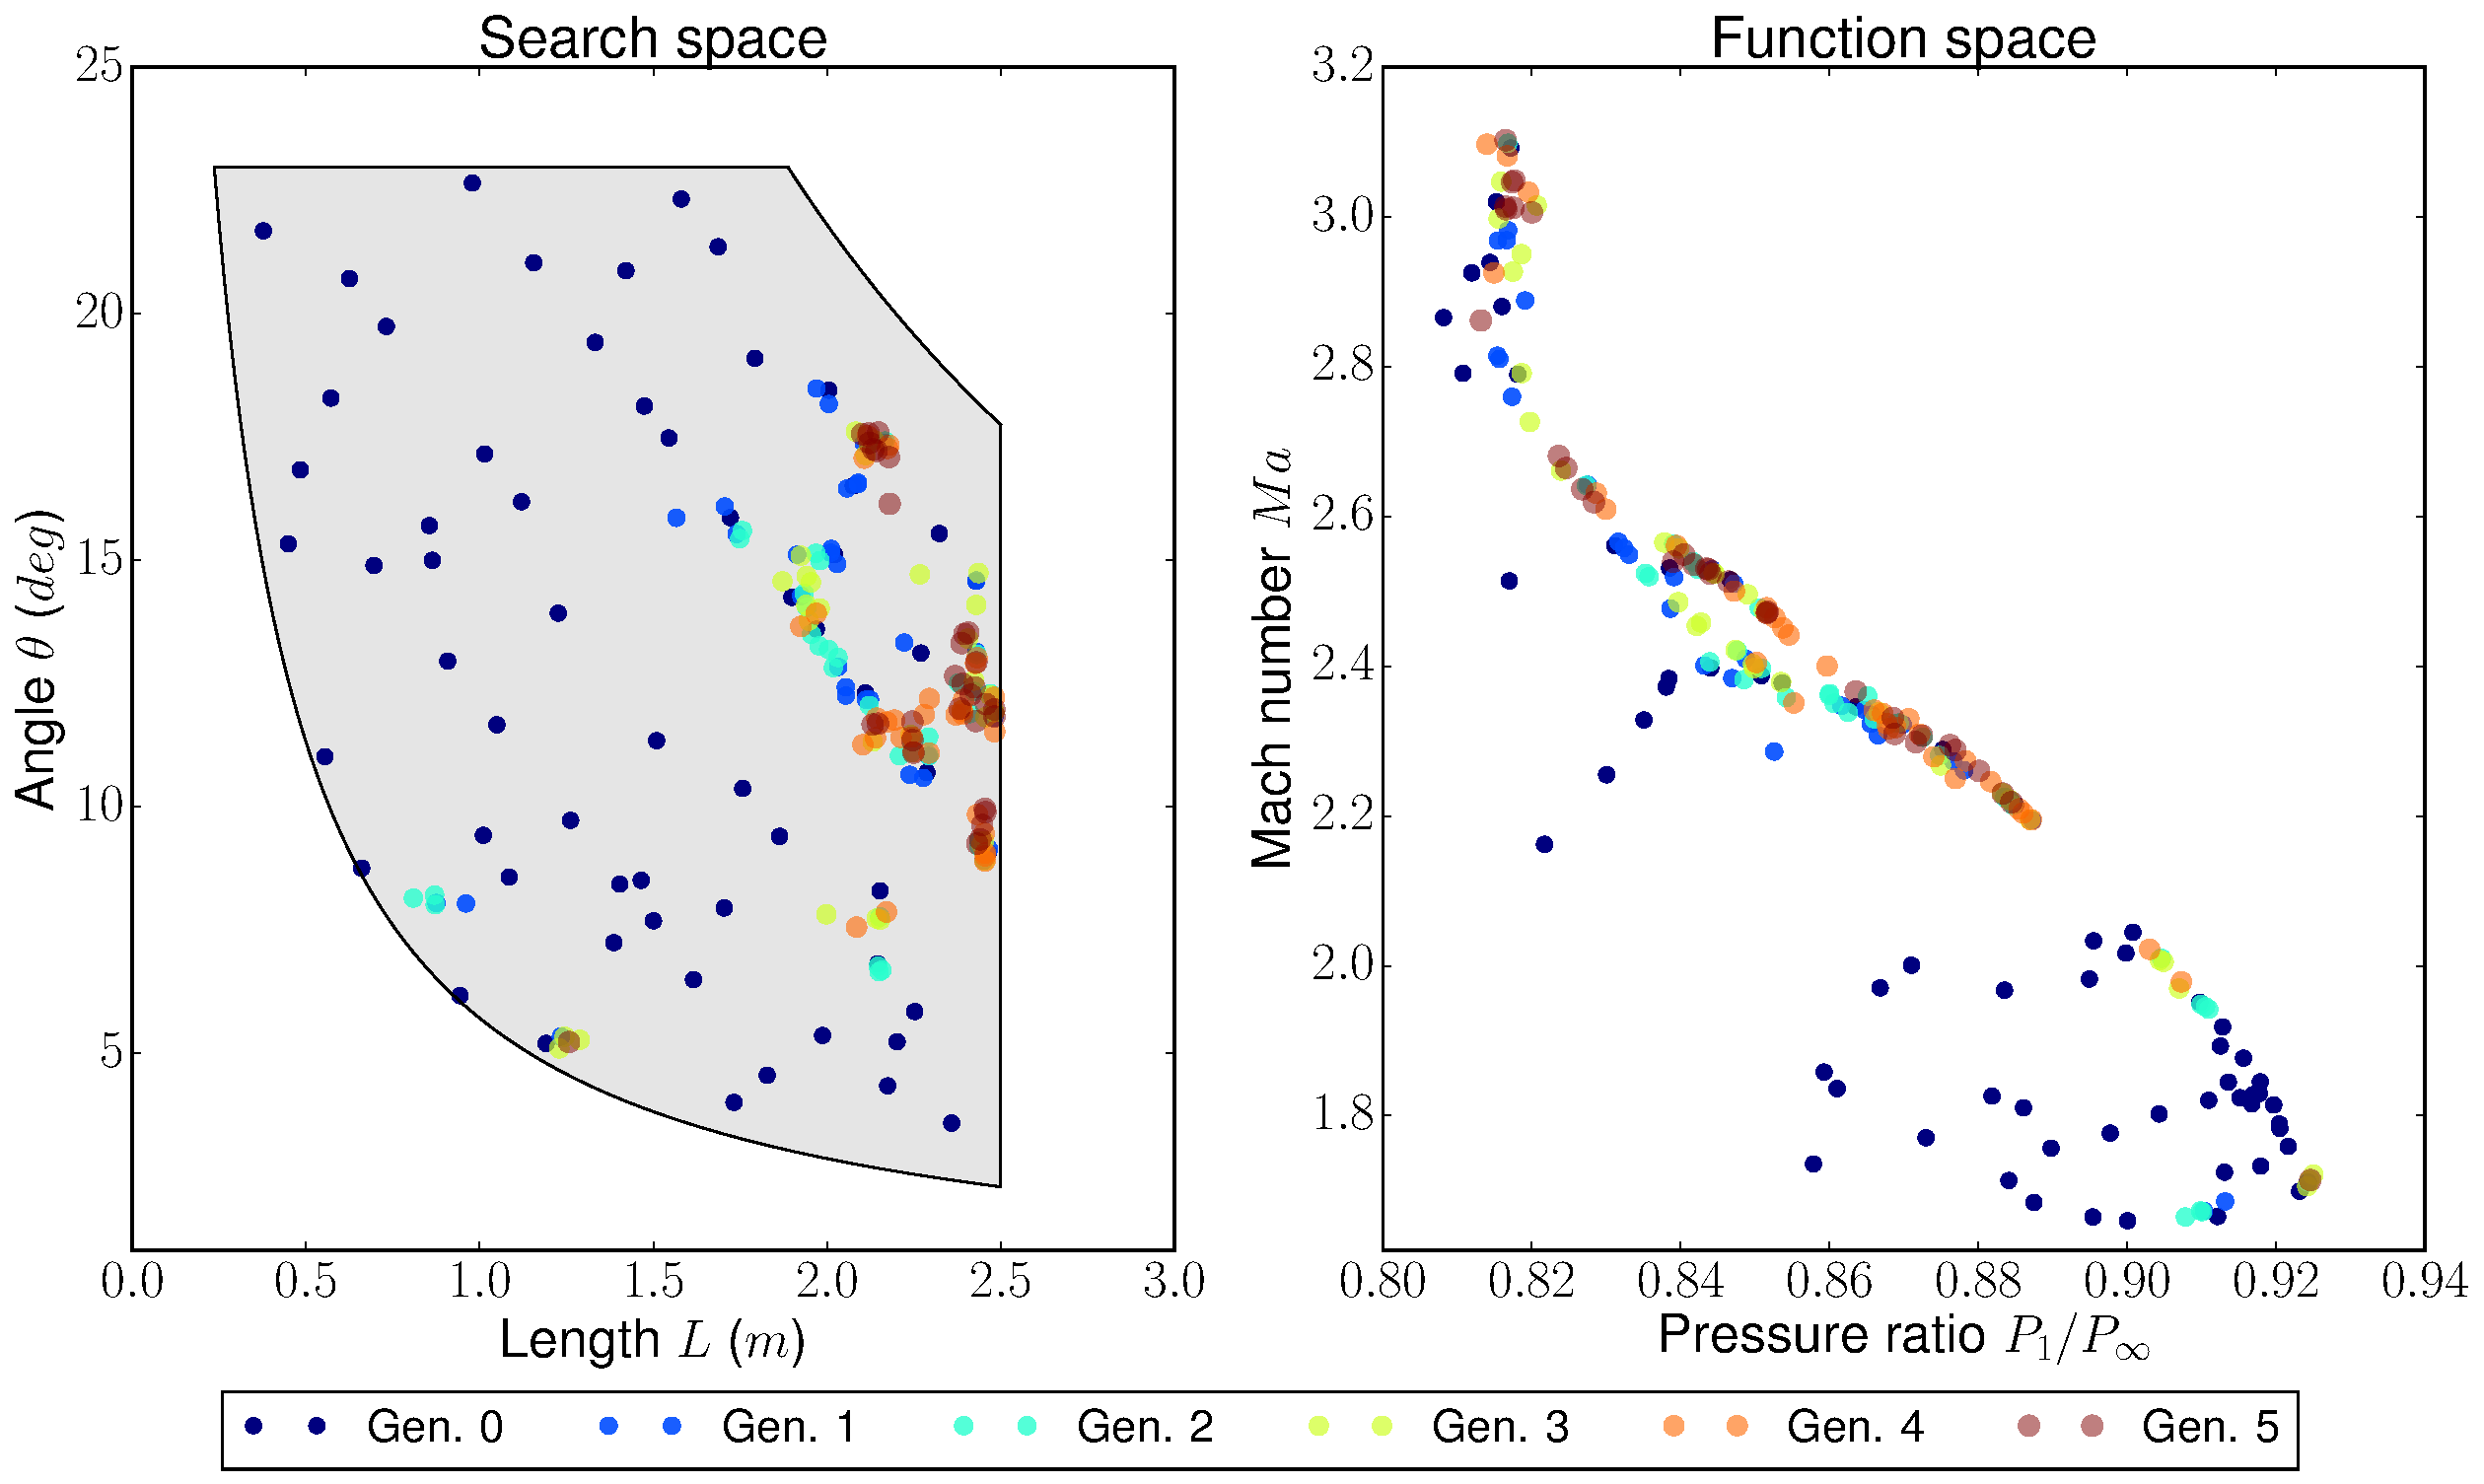
\includegraphics[height=0.35\textheight, width=\textwidth]{Figures/4/gen5.pdf}
        \caption{Evolution of the generations for the diffuser case}
        \label{fig:genForDifusser}
    \end{figure}

\begin{figure}[h!]
    \centering
    \begin{subfigure}[t]{0.31\textwidth}
        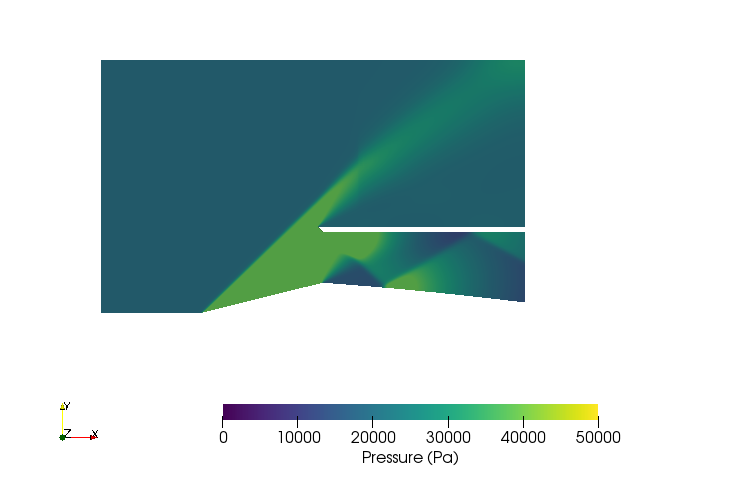
\includegraphics[width=0.95\textwidth, height=0.18\textheight]{Figures/4/SCpg0i3.png}
    \end{subfigure}
    \begin{subfigure}[t]{0.31\textwidth}
        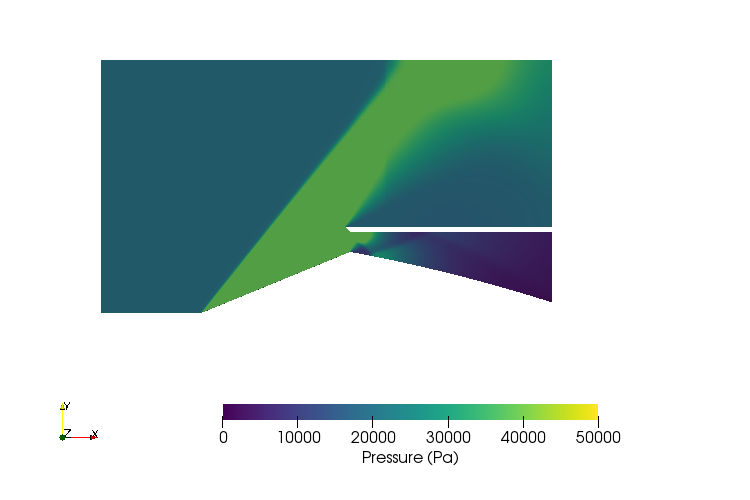
\includegraphics[width=0.95\textwidth, height=0.18\textheight]{Figures/4/SCpg0i9.png}
    \end{subfigure}
    \begin{subfigure}[t]{0.31\textwidth}
        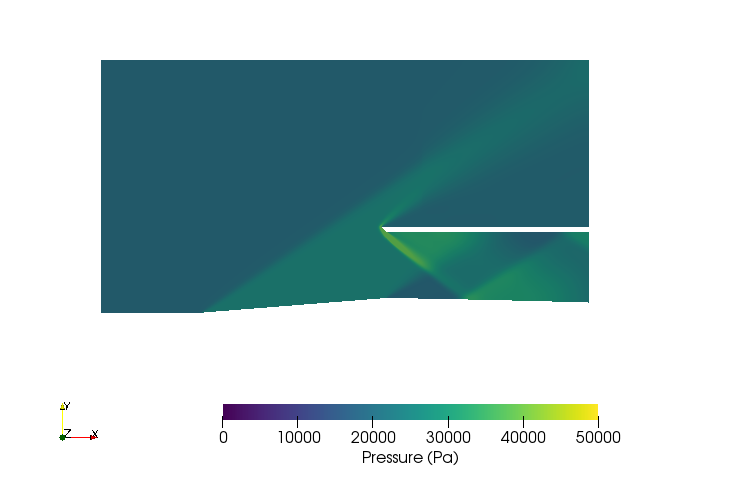
\includegraphics[width=0.95\textwidth, height=0.18\textheight]{Figures/4/SCpg0i46.png}
    \end{subfigure}
    \caption{Sample of the initial generation for the diffuser case}
            \label{fig:initialDif}
\end{figure}

\begin{figure}[h!]
    \centering
    \begin{subfigure}[t]{0.31\textwidth}
        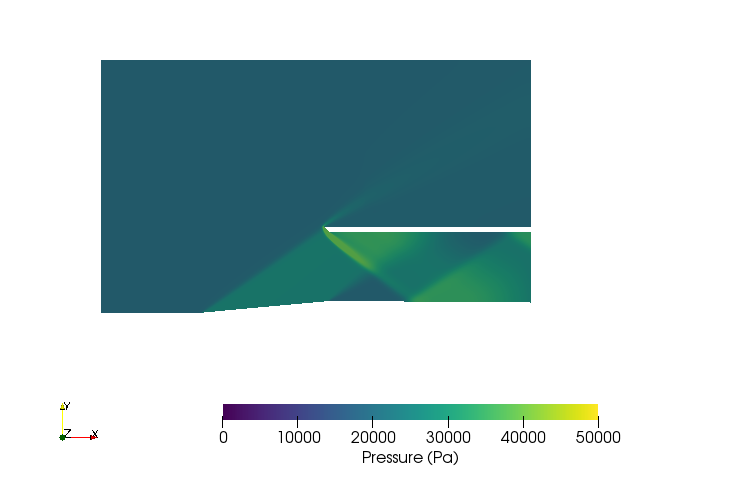
\includegraphics[width=0.95\textwidth, height=0.18\textheight]{Figures/4/SCpg5i9.png}
    \end{subfigure}
    \begin{subfigure}[t]{0.31\textwidth}
        \includegraphics[width=0.95\textwidth, height=0.18\textheight]{Figures/4/SCpg5i14.png}
    \end{subfigure}
    \begin{subfigure}[t]{0.31\textwidth}
        \includegraphics[width=0.95\textwidth, height=0.18\textheight]{Figures/4/SCpg5i18.png}
    \end{subfigure}
    \caption{Sample of the final generation for the diffuser case}
    \label{fig:finalDif}
\end{figure}


\newpage

\subsubsection*{Airfoil design: lift maximization and drag minimization}

     \begin{figure}[h!]
        \centering
        \small
        \includegraphics[width=\textwidth, height=0.4\textheight]{Figures/4/cLcDgen10.png}
        \caption{Evolution of the generations for the airfoil case I}
        \label{fig:genForCLCD}
    \end{figure}


\begin{figure}[h!]
    \centering
    \begin{subfigure}[t]{0.31\textwidth}
        \includegraphics[width=0.95\textwidth, height=0.17\textheight]{Figures/4/g0i116.png}
    \end{subfigure}
    \begin{subfigure}[t]{0.31\textwidth}
        \includegraphics[width=0.95\textwidth, height=0.17\textheight]{Figures/4/g0i19.png}
    \end{subfigure}
    \begin{subfigure}[t]{0.31\textwidth}
        \includegraphics[width=0.95\textwidth, height=0.17\textheight]{Figures/4/g0i55.png}
    \end{subfigure}
    \caption{Sample of the initial generation for the airfoil case I}
    \label{fig:initialCLCD}
\end{figure}

\begin{figure}[h!]
    \centering
    \begin{subfigure}[t]{0.31\textwidth}
        \includegraphics[width=0.95\textwidth, height=0.17\textheight]{Figures/4/g10i14.png}
    \end{subfigure}
    \begin{subfigure}[t]{0.31\textwidth}
        \includegraphics[width=0.95\textwidth, height=0.17\textheight]{Figures/4/g10i35.png}
    \end{subfigure}
    \begin{subfigure}[t]{0.31\textwidth}
        \includegraphics[width=0.95\textwidth, height=0.17\textheight]{Figures/4/g10i55.png}
    \end{subfigure}
    \caption{Sample of the final generation for the airfoil case I}
    \label{fig:finalCLCD}
\end{figure}

    
\subsubsection*{Airfoil design: lift-to-drag ratio and area maximization}

     \begin{figure}[h!]
        \centering
        \small
        \includegraphics[width=\textwidth, height=0.4\textheight]{Figures/4/LDgen10.png}
        \caption{Evolution of the generations for the airfoil case II}
        \label{fig:genForLD}
    \end{figure}
    
    
    \begin{figure}[h!]
    \centering
    \begin{subfigure}[t]{0.31\textwidth}
        \includegraphics[width=0.95\textwidth, height=0.17\textheight]{Figures/4/LDAg0i23.png}
    \end{subfigure}
    \begin{subfigure}[t]{0.31\textwidth}
        \includegraphics[width=0.95\textwidth, height=0.17\textheight]{Figures/4/LDAg0i99.png}
    \end{subfigure}
    \begin{subfigure}[t]{0.31\textwidth}
        \includegraphics[width=0.95\textwidth, height=0.17\textheight]{Figures/4/LDAg0i107.png}
    \end{subfigure}
    \caption{Sample of the initial generation for the airfoil case II}
    \label{fig:initialLD}
\end{figure}

\begin{figure}[h!]
    \centering
    \begin{subfigure}[t]{0.31\textwidth}
        \includegraphics[width=0.95\textwidth, height=0.17\textheight]{Figures/4/LDAg10i11.png}
    \end{subfigure}
    \begin{subfigure}[t]{0.31\textwidth}
        \includegraphics[width=0.95\textwidth, height=0.17\textheight]{Figures/4/LDAg10i47.png}
    \end{subfigure}
    \begin{subfigure}[t]{0.31\textwidth}
        \includegraphics[width=0.95\textwidth, height=0.17\textheight]{Figures/4/LDAg10i53.png}
    \end{subfigure}
    \caption{Sample of the final generation for the airfoil case II}
    \label{fig:finalLD}
\end{figure}

\chapter{Discussion}

Once the results of all the four optimizations performed have been shown, they will be briefly discussed. The four cases showed how the individuals of the populations move throughout the search space with its corresponding position in the function space. Also, some sample individuals of the population are presented in order to see how the individuals behave and how they evolve towards a solution. 

\subsubsection*{Supression of cylinder vortex oscillations}

The search space is too large and, due to time restrictions, the number of individuals simulated did not cover widely the search domain. Also, the solution converges to two points instead of a full Pareto front. The algorithm, however, behaves as it should, because it moves the points towards the zero oscillations points, which is not reached but it is close to some solutions. 

In Figure \ref{fig:initialCyl} some individuals from the first population have been randomly chosen and the figures with its oscillations are shown. The blue line represents the sum of the pressure and viscous force in the $x$ axis while the green line is the pressure and viscous force in the $y$ axis. The horizontal axis represents the time evolution while the vertical axis is the force in Newtons. The last point is chosen as a reference to pick a number of cycles that realistically represents the oscillations suffered by the cylinder. As it can be seen, there is a great variety of amplitudes and frequencies in the search space.

In Figure \ref{fig:finalCyl} the force plots for the two points where the algorithm converges are shown. The oscillations have been damped and the amplitude is smaller than the amplitudes of the initial population which was the objective of the algorithm. Thus it can be said that, although not being a Pareto front, the solutions of the algorithm have reduced the amplitude of the oscillations. 

\subsubsection*{Inlet to diffuser geometry}

In this case, Figure \ref{fig:genForDifusser} shows not only the evolution of the individuals but also the search space where they are bounded in. In contrast with the cylinder analysis, the function space shows a neat and well-defined Pareto front. The individuals may have a large pressure ratio and a low Mach number or a large Mach number and a small pressure ratio: the trade-off between the two variables has been captured.

In Figure \ref{fig:initialDif} some randomly chosen individuals from the initial generation are chosen. It can be seen that there is a great variety of $L$ and $\theta$ possible values. The cases shown do not look as optimal, and there are shapes (as the middle one) that look even unrealistic. However, in Figure \ref{fig:finalDif} it can be seen how the individuals have evolved towards a most optimal solution. The left image shows the expected solution where the shock wave hits the cowl of the engine. However, there are plenty of other solutions that are not-dominated, having higher $Ma$ for some cases and higher pressure ratios for others. 

\subsubsection*{Airfoil design: lift maximization and drag minimization}


Given that the airfoil setup was quicker than the other cases, much more individuals have been simulated (see Figure \ref{fig:genForCLCD}). The search space is well covered and the points are spread enough to see where the optimal region is. Points eventually converge to the location of that optimal area, creating some unwanted clustering zones. This is translated in the function spaces as a well-defined Pareto front that captures the trade-off between lift and drag, given that both are related. 

In Figure \ref{fig:initialCLCD} it can be seen that there is a wide range of possible airfoils obtained through the Joukowsky transform. This case was initialized with a Sobol sampling, which is quasi-random low discrepancy initialization that tries to cover the whole search space as much as possible. This initialization will be useful for the second optimization performed to the airfoil case, given that the same initial population was used to reduce as much as possible computational time. This type of initialization covers better the search space and, while for a genetic algorithm not applied to CFD this will yield the same results after a large enough number of generations, in this case, it is very interesting to reduce the simulations as much as possible. The wide variety of airfoils in the first generation have converged to more aerodynamic shapes (see Figure \ref{fig:finalCLCD}) with a low thickness and slightly cambered. This shape enhances as much as possible the lift while affecting the less possible the drag. 


\subsubsection*{Airfoil design: lift-to-drag and area maximization}

Finally, Figure \ref{fig:genForLD} shows the search space (which is the same as the previous one) and the function space with a completely different Pareto front as the one seen in Figure \ref{fig:genForCLCD}. Although the first generation was formed by the same individuals, the selection pressure based on assigning the fitness depending on different objectives yield completely opposed results. The Pareto front is well captured and it shows the most optimal solutions for maximizing the $L/D$ ratio and the area. 

Figure \ref{fig:initialLD} shows randomly chosen individuals from the initial generation with some possible airfoils (having that individuals from Figure \ref{fig:initialCLCD} also are possible individuals from the first generation for the airfoil case II). The results of the final generation (see Figure \ref{fig:finalLD}) are way different from the results of Figure \ref{fig:finalCLCD}. Here the thickness is (in general) larger than in the previous case. However, there are individuals that have a smaller thickness than other individuals from the population - but being still thicker than the individuals in Figure \ref{fig:finalCLCD}. This shows that the optimization process has been successfully completed. 
\chapter{Conclusions and further developments}

As it can be seen, genetic algorithms are a great approach to all kind of optimization problems: from CFD cases with multiobjective optimization to single objective optimization of other engineering systems. The results obtained show that this approach is (although time-consuming) efficient compared with other approaches. Genetic algorithms can be not very efficient, computationally speaking. But they are the only approach to some problems as global optimization because methods like gradient search only locate local minimum. Genetic algorithms may also be applied to black-box functions, where only an evaluation from the function is required. 

The results shown in the Figures \ref{fig:genForDifusser}, \ref{fig:genForCLCD} and \ref{fig:genForLD} have the Pareto front correctly captured with the NSGA-II. However, there are zones in the Pareto front that are not correctly covered, leaving gaps in the non-dominated set and having areas with sparse individuals combined with very populated areas. There are different ways to improve these behaviors and before applying the algorithm to other cases, a refinement should be done to eliminate these discrepancies \cite{chichakly2013improving} \cite{yuan2014improved}. However, these problems may be due to a little number of individuals and/or generations, having that larger numbers will give a more detailed and evenly distributed Pareto front.

The algorithm has proved to be robust in the sense that if there is a function space without a Pareto front, it will converge to the most optimal solutions, as done in the cylinder case. Nevertheless, this lack of Pareto front may also be due to a small population size. Cylinder case also requires a more in-depth analysis to extract more information from the data, such as the frequencies of the oscillations. With this detailed analysis, other parameters may be chosen for achieving better performance in the optimization and smaller oscillations in the flow.

Complex search spaces have been also analyzed within this analysis and the results are that genetic algorithms may perform optimization in constrained problems. Although the constraints were only imposed in the search space, the NSGA-II also allows the use of constraints in the function space \cite{deb2002fast}.

The adaptability of the code is one of the most powerful characteristics of this optimization method. Slight changes in the code (just replacing some variables) will allow the code to optimize different objectives, as it was shown with the airfoil case. This makes the code versatile and open to a broad variety of possibilities when looking for new optimization problems.

Although genetic algorithms have been presented as one of the better solutions, they also have problems and limitations. The most evident one is that GA are heuristic methods that only achieve an approximation of the actual solution. Due to the stochasticity of the algorithm, each run will return a slightly different approximation of that solution. However, finding the "optimal" solution may not be feasible and the solution obtained with genetic algorithms may consist of a robust solution for multi-objective purposes. 

There are other evolutionary algorithms that may also be implemented for CFD optimization, such as evolutionary algorithms or particle swarm optimization. All these new machine learning techniques will be of high importance in the future of computer fluid simulation and the optimization of cases, codes, and shapes. 

Another major improvement that may be done to the application of genetic algorithms in the computer fluid dynamics field is data management. Each simulation returns a huge amount of data (roughly $50\ Gb$ per case) and everything is reduced to just some bytes that contain the fitness value. Taking advantage of all the data of the simulations may be used for improving the convergence of the algorithm without being necessary the use of more generations or individuals. 

Another update in the code can be a higher parallelization level. Evolutionary algorithms have the advantage to be easily and efficiently parallelizable \cite{thevenin2008and}. The code only performs the CFD simulations in a parallel fashion. However, fitness evaluation (extracting data from the simulations) is also a very computer demanding operation. If this process was also run in parallel instead of in serial processors, the whole algorithm will run in shorter amounts of time. The big bottleneck of genetic algorithms in computer fluid dynamics is exactly this: the evaluation time of each individual is high when repeating it generation after generations. Analysis like processor convergence are more than justified to reduce as much as possible the simulation time.

The use of genetic algorithms in 3D simulations is possible, but the increase in computational time make it an unfeasible analysis for this report. The amount of data from a 3D simulation will also be way larger than the data of a 2D simulation, being necessary more space to handle all the files. Apart from computational limitations, the use of GA in 3D cases will also be a topic of high importance in the future.

Finally, the algorithm has been implemented for 2 variables and 2 objective functions. However, the real potential of the genetic algorithm lays on cases with more than two variables, where the search space is complex and can not be visualized in 2 dimensions. This search will also require higher computational resources and more time will be spent in doing simulations. In 2D cases, the results may seem more or less intuitive and the Pareto front may be 'located' in both the search and function space. In the case of tenths of variables, this visualization will be a little trickier and the direct relationship between search and function spaces will not be that straightforward. 

%%now enable appendix numbering format and include any appendices
\appendix
\chapter{Gantt diagram}

This appendix has the Gantt diagram with the distribution of time spend along the project, structured by tasks. Simulation time has been included but it has not been added up.
    
    \begin{figure}[h!]
        \centering
        \includegraphics[width=1\textwidth]{Figures/others/GanttDiagram.pdf} 
        \caption{Gantt chart with the project schedule}
        \label{fig:Gantt}
    \end{figure}    

%\include{appendix2}

%next line adds the Bibliography to the contents page
\addcontentsline{toc}{chapter}{Bibliography}
%uncomment next line to change bibliography name to references
\renewcommand{\bibname}{References}
%\bibliography{refs}        %use a bibtex bibliography file refs.bib
%\bibliographystyle{ieee}  %use the plain bibliography style

\nocite{*}
\printbibliography

\end{document}

